\section{Experimental Evaluation}
\subsection{Setup}

The setup used in training the baseline and the RNN is identical. Both networks are based upon layers from the VGGNet and the weights of the layers are pre-trained on ILSVRC data set for several weeks. It is beneficial to apply the pre-trained weights and use the principle of transfer learning instead of learning the weights from scratch. 

According to the literature \cite{stand_cnn_notes_1}, there are several approaches to perform transfer-learning. Among these is a strategy to remove the final fully connected layer of the network. Then the pre-trained CNN is applied as a feature extractor for a new fully connected layer which fits the number of classes in the data set.
A second strategy is carry out the first strategy and fine-tune a selected set of weights in the pre-trained CNN.

The chosen strategy in this setup was to remove and create a new final fully connected layer which fit the number of sleep stages in both networks. Instead of fine-tuning the weights in the other fully connected layers, it has been chosen to train the dropout operations between those layers in order to prevent overfitting. 

The weights in the LSTM cell have been trained from scratch. The weights in the forget bias have been initialized to $1$ which entails the LSTM cell to have no prior knowledge.
%This strategy is different compared to the setup in \cite{main_ar}. They re-train all the weights in the fully connected layers.

During the training process the networks only have access to the current epoch. This is different from the setup in \cite{main_ar} where the network use two prior epochs and two posterior epochs in order to learn the current epoch. The reason for this choice was due to real time considerations. If the classifier should work in real time then it does not have any posterior epochs to work with. 
It is possible to use prior epochs in real time classifications and it can be considered as future research.

Both the CNN and the RNN networks have been optimized in order to minimize their categorical cross-entropy. Their loss function is handled by the AdamOptimizer, provided by TF, which iterates over a mini-batch with a size of 32. 
The training process has been repeated for 20 training epochs. The learning rate has been initialized to $10^{-5}$ and its decay rate, first and second order moment have not been changed from default.

Due to the characteristic of the sleep stages, the classes shown in table \ref{tab_class_balance} are not equally distributed. The selected choice for fixing the issue is to randomly down-sample the majority classes to fit the minority class in each training epoch. A similar approach has been applied in \cite{main_ar}. 

The setup is capable of performing leave-one-out cross-validation due to the relative small number of subjects and a few professionel skilled sleep stage experts.
The subjects have been divided into test, train and validation. Subject 19 and subject 20 have been fixed to the validation set in order to get the $10\%$ of the total amount. 

The test subject for the first fold is subject one. The train data includes subject 2 to subject 18. Due to time considerations it was chosen only to perform the first fold.

\subsection{Results}
\label{subsec:results}

Table \ref{tab_res_1} summarizes the performances evaluated for the two validation subjects in both networks. 
The first column block reports the confusion matrix. The next block reports the normalized confusion matrix. The third block reports the following per-class metrics: Precision, sensitivity, F$_1$-score and accuracy. The accuracy is not a reliable metric of the performance in this project, yield to misleading results of the imbalanced sleep stages in the validation set \cite[sec. 11]{dl_book}.

\begin{table*}[th!]
\centering
\begin{tabular}{ll | llllll | llllll | llll}
                     &    & \multicolumn{6}{c}{Predicted} & \multicolumn{6}{| c}{Normalized pred. (in \%)}  & \multicolumn{4}{| c}{Per-class metric (in \%)} \\
                     &    & W  & N1  & N2  & N3  & N4 & R & W & N1 & N2 & N3 & N4 & R & Pre.       & Sen.      & F$_1$      & Acc.      \\\hline
\multirow{6}{*}{CNN} & W  &495 & 145 & 29 & 11 & 1 & 20 & 71 & 21 & 4 & 2 & 0 & 3 & 91 & 71 & 80 & 93 \\ 
                     & N1 &    25 & 211 & 43 & 0 & 0 & 62 & 7 & 62 & 13 & 0 & 0 & 18 & 43 & 62 & 51 & 89 \\ 
                     & N2 &    4 & 51 & 1313 & 104 & 17 & 68 & 0 & 3 & 84 & 7 & 1 & 4 & 91 & 84 & 88 & 90 \\ 
                     & N3 &    0 & 2 & 11 & 164 & 64 & 0 & 0 & 1 & 5 & 68 & 27 & 0 & 49 & 68 & 57 & 93 \\ 
                     & N4 &    0 & 0 & 0 & 54 & 91 & 0 & 0 & 0 & 0 & 37 & 63 & 0 & 53 & 63 & 57 & 96 \\ 
                     & R  &    17 & 80 & 46 & 0 & 0 & 591 & 2 & 11 & 6 & 0 & 0 & 81 & 80 & 81 & 80 & 92 \\ \hline
\multirow{6}{*}{RNN} & W  &    578 & 39 & 26 & 7 & 1 & 43 & 83 & 6 & 4 & 1 & 0 & 6 & 89 & 83 & 86 & 95 \\ 
                     & N1 &    38 & 107 & 64 & 0 & 0 & 132 & 11 & 31 & 19 & 0 & 0 & 39 & 55 & 31 & 40 & 91 \\ 
                     & N2 &    8 & 13 & 1314 & 102 & 28 & 92 & 1 & 1 & 84 & 7 & 2 & 6 & 90 & 84 & 87 & 89 \\ 
                     & N3 &    3 & 0 & 18 & 125 & 95 & 0 & 1 & 0 & 7 & 52 & 39 & 0 & 43 & 52 & 47 & 92 \\ 
                     & N4 &    0 & 0 & 1 & 60 & 84 & 0 & 0 & 0 & 1 & 41 & 58 & 0 & 40 & 58 & 48 & 95 \\ 
                     & R  &    19 & 36 & 43 & 0 & 0 & 636 & 3 & 5 & 6 & 0 & 0 & 87 & 70 & 87 & 78 & 90
\end{tabular}
\caption{This table report the confusion matrix, its normalized confusion matrix and selected performances metrics for the CNN and RNN network.}
\label{tab_res_1}
\end{table*}

The baseline, reported in table \ref{tab_res_1}, classifies the sleep stage N2 with a sensitivity of $84\%$. Then followed by R, W, N3, N4 and N1. N1 with a sensitivity of $62\%$ as the most difficult sleep stage to classify. The highest misclassification error is achieved in N3 with a sensitivity of $37\%$.

The RNN classifies the sleep stage R with the highest sensitivity ($87\%$). Then followed by N2, W, N4, N3 and N1. N1 with a sensitivity of $31\%$ as the most difficult sleep stage to classify.

The precision metrics for the CNN and the RNN are relatively low for sleep stage N3 and sleep stage N4 compared to the other sleep stages. The misclassification rates for N3 and N4 are relatively close to its classification rates. 
The visual illustrations of the stages are similar, which can be a logical explanation for merging N3 and N4 together into one sleep stage as in the newest definition \cite{AASM}.

%precision: fraction which were deteced correct. 
%sensitivity: fraction of ture events that was detected correct.. percentage of sick people who are correctly identified as having the condition.. the probability of a correct detection...
%F1 score: precision can be traded for sensitivity.. to summerise this score, it is possible to convert the precision and sensitivy into one number -> f1 score..

%\todo[inlin]{Precision: Reduce FN and increasing TP. This focus on the cluster of positive..}
%\todo[inlin]{Sensitivity: tries to hard reduce FN and increase TP}
%\todo[inlin]{F1: A combination between precision and sensitivity.}

Table \ref{tab_res_2} reports the mean values and its corresponding $95\%$ confident values computed by bootstrapping. There has been applied $100.000$ bootstrap iterations with replacement in order to compute the average performance metrics for the two networks.
\begin{table}[th!]
\centering
\begin{tabular}{l | llll}
Study & Precision & Sensitivity & F$_1$-score & Accuracy \\\hline
FE \cite{main_ar} & 90-\textbf{91}-93 & 70-\textbf{73}-77 & 78-\textbf{81}-83 & 81-\textbf{83}-85\\
FT \cite{main_ar} & 92-\textbf{93}-94 & 75-\textbf{78}-81 & 82-\textbf{84}-86 & 84-\textbf{86}-88\\\hline
CNN               & 65-\textbf{68}-70 & 71-\textbf{71}-72 & 67-\textbf{69}-70 & 92-\textbf{92}-92\\
RNN               & 62-\textbf{65}-67 & 63-\textbf{66}-69 & 62-\textbf{64}-67 & 92-\textbf{92}-92
\end{tabular}
\caption{\textbf{Mean} and corresponding $95\%$ confident values computed by 100.000 bootstrap iterations with replacement. The two first rows are metrics from \cite{main_ar}.}
\label{tab_res_2}
\end{table}
According to table \ref{tab_res_2} it can be concluded that the RNN does not outperform the baseline network w.r.t. the selected performance metrics.

%\subsubsection{Hypnograms}
%\begin{figure*}[th!]
%\centering
%\begin{subfigure}{1\textwidth}
\centering
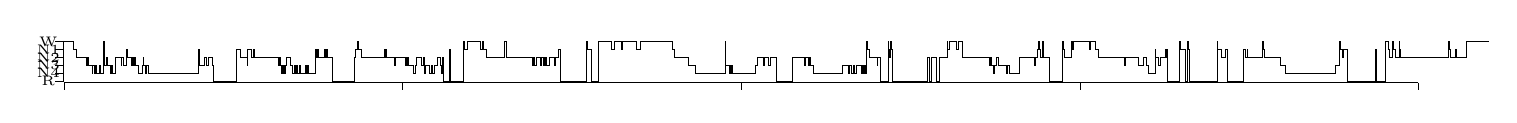
\begin{tikzpicture}[] 
\draw[line width=0.1mm] (0,-0.52)--(17.20, -0.52);
\draw[line width=0.1mm] (0,-0.52)--(0,-0.62);
\draw[line width=0.1mm] (8.60,-0.52)--(8.60,-0.62);
\draw[line width=0.1mm] (17.20,-0.52)--(17.20,-0.62);
\draw[line width=0.1mm] (4.3,-0.52)--(4.3,-0.62);
\draw[line width=0.1mm] (12.9,-0.52)--(12.9,-0.62);
\draw[line width=0.1mm] (-0.01,0.01)--(-0.01,-0.51);
\draw[line width=0.1mm] (-0.01,-0.0)--(-0.11,-0.0);
\draw[line width=0.1mm] (-0.01,-0.1)--(-0.11,-0.1);
\draw[line width=0.1mm] (-0.01,-0.2)--(-0.11,-0.2);
\draw[line width=0.1mm] (-0.01,-0.3)--(-0.11,-0.3);
\draw[line width=0.1mm] (-0.01,-0.4)--(-0.11,-0.4);
\draw[line width=0.1mm] (-0.01,-0.5)--(-0.11,-0.5);
\node at (-0.2,-0.0)   (a) {{\fontsize{2.5}{4}\selectfont W}};
\node at (-0.2,-0.1)   (a) {{\fontsize{2.5}{4}\selectfont N1}};
\node at (-0.2,-0.2)   (a) {{\fontsize{2.5}{4}\selectfont N2}};
\node at (-0.2,-0.3)   (a) {{\fontsize{2.5}{4}\selectfont N3}};
\node at (-0.2,-0.4)   (a) {{\fontsize{2.5}{4}\selectfont N4}};
\node at (-0.2,-0.5)   (a) {{\fontsize{2.5}{4}\selectfont R}};
\draw[line width=0.05mm] (0.00,0.0)--(0.01,0.0)--(0.01,0.0)--(0.02,0.0)--(0.02,0.0)--(0.03,0.0)--(0.03,0.0)--(0.04,0.0)--(0.04,0.0)--(0.05,0.0)--(0.05,0.0)--(0.06,0.0)--(0.06,0.0)--(0.07,0.0)--(0.07,0.0)--(0.08,0.0)--(0.08,0.0)--(0.09,0.0)--(0.09,0.0)--(0.10,0.0)--(0.10,0.0)--(0.11,0.0)--(0.11,-0.1)--(0.12,-0.1)--(0.12,-0.1)--(0.13,-0.1)--(0.13,-0.1)--(0.14,-0.1)--(0.14,-0.1)--(0.15,-0.1)--(0.15,-0.2)--(0.16,-0.2)--(0.16,-0.2)--(0.17,-0.2)--(0.17,-0.2)--(0.18,-0.2)--(0.18,-0.2)--(0.19,-0.2)--(0.19,-0.2)--(0.20,-0.2)--(0.20,-0.2)--(0.21,-0.2)--(0.21,-0.2)--(0.22,-0.2)--(0.22,-0.2)--(0.23,-0.2)--(0.23,-0.2)--(0.24,-0.2)--(0.24,-0.2)--(0.25,-0.2)--(0.25,-0.2)--(0.26,-0.2)--(0.26,-0.2)--(0.27,-0.2)--(0.27,-0.2)--(0.28,-0.2)--(0.28,-0.30000000000000004)--(0.29,-0.30000000000000004)--(0.29,-0.2)--(0.30,-0.2)--(0.30,-0.30000000000000004)--(0.31,-0.30000000000000004)--(0.31,-0.30000000000000004)--(0.32,-0.30000000000000004)--(0.32,-0.30000000000000004)--(0.33,-0.30000000000000004)--(0.33,-0.30000000000000004)--(0.34,-0.30000000000000004)--(0.34,-0.30000000000000004)--(0.35,-0.30000000000000004)--(0.35,-0.4)--(0.36,-0.4)--(0.36,-0.30000000000000004)--(0.37,-0.30000000000000004)--(0.37,-0.30000000000000004)--(0.38,-0.30000000000000004)--(0.38,-0.4)--(0.39,-0.4)--(0.39,-0.4)--(0.40,-0.4)--(0.40,-0.30000000000000004)--(0.41,-0.30000000000000004)--(0.41,-0.4)--(0.42,-0.4)--(0.42,-0.4)--(0.43,-0.4)--(0.43,-0.4)--(0.44,-0.4)--(0.44,-0.4)--(0.45,-0.4)--(0.45,-0.30000000000000004)--(0.46,-0.30000000000000004)--(0.46,-0.4)--(0.47,-0.4)--(0.47,-0.4)--(0.48,-0.4)--(0.48,-0.4)--(0.49,-0.4)--(0.49,-0.4)--(0.50,-0.4)--(0.50,0.0)--(0.51,0.0)--(0.51,-0.30000000000000004)--(0.52,-0.30000000000000004)--(0.52,-0.30000000000000004)--(0.53,-0.30000000000000004)--(0.53,-0.2)--(0.54,-0.2)--(0.54,-0.2)--(0.55,-0.2)--(0.55,-0.30000000000000004)--(0.56,-0.30000000000000004)--(0.56,-0.30000000000000004)--(0.57,-0.30000000000000004)--(0.57,-0.30000000000000004)--(0.58,-0.30000000000000004)--(0.58,-0.30000000000000004)--(0.59,-0.30000000000000004)--(0.59,-0.4)--(0.60,-0.4)--(0.60,-0.30000000000000004)--(0.61,-0.30000000000000004)--(0.61,-0.4)--(0.62,-0.4)--(0.62,-0.4)--(0.63,-0.4)--(0.63,-0.4)--(0.64,-0.4)--(0.64,-0.4)--(0.65,-0.4)--(0.65,-0.2)--(0.66,-0.2)--(0.66,-0.2)--(0.67,-0.2)--(0.67,-0.2)--(0.68,-0.2)--(0.68,-0.2)--(0.69,-0.2)--(0.69,-0.2)--(0.70,-0.2)--(0.70,-0.2)--(0.71,-0.2)--(0.71,-0.2)--(0.72,-0.2)--(0.72,-0.30000000000000004)--(0.73,-0.30000000000000004)--(0.73,-0.2)--(0.74,-0.2)--(0.74,-0.2)--(0.75,-0.2)--(0.75,-0.30000000000000004)--(0.76,-0.30000000000000004)--(0.76,-0.30000000000000004)--(0.77,-0.30000000000000004)--(0.77,-0.30000000000000004)--(0.78,-0.30000000000000004)--(0.78,-0.30000000000000004)--(0.79,-0.30000000000000004)--(0.79,-0.1)--(0.80,-0.1)--(0.80,-0.2)--(0.81,-0.2)--(0.81,-0.2)--(0.82,-0.2)--(0.82,-0.2)--(0.83,-0.2)--(0.83,-0.2)--(0.84,-0.2)--(0.84,-0.2)--(0.85,-0.2)--(0.85,-0.30000000000000004)--(0.86,-0.30000000000000004)--(0.86,-0.30000000000000004)--(0.87,-0.30000000000000004)--(0.87,-0.2)--(0.88,-0.2)--(0.88,-0.30000000000000004)--(0.89,-0.30000000000000004)--(0.89,-0.2)--(0.90,-0.2)--(0.90,-0.30000000000000004)--(0.91,-0.30000000000000004)--(0.91,-0.30000000000000004)--(0.92,-0.30000000000000004)--(0.92,-0.30000000000000004)--(0.93,-0.30000000000000004)--(0.93,-0.30000000000000004)--(0.94,-0.30000000000000004)--(0.94,-0.4)--(0.95,-0.4)--(0.95,-0.4)--(0.96,-0.4)--(0.96,-0.4)--(0.97,-0.4)--(0.97,-0.4)--(0.98,-0.4)--(0.98,-0.4)--(0.99,-0.4)--(0.99,-0.30000000000000004)--(1.00,-0.30000000000000004)--(1.00,-0.2)--(1.01,-0.2)--(1.01,-0.30000000000000004)--(1.02,-0.30000000000000004)--(1.02,-0.30000000000000004)--(1.03,-0.30000000000000004)--(1.03,-0.4)--(1.04,-0.4)--(1.04,-0.30000000000000004)--(1.05,-0.30000000000000004)--(1.05,-0.30000000000000004)--(1.06,-0.30000000000000004)--(1.06,-0.30000000000000004)--(1.07,-0.30000000000000004)--(1.07,-0.4)--(1.08,-0.4)--(1.08,-0.4)--(1.09,-0.4)--(1.09,-0.4)--(1.10,-0.4)--(1.10,-0.4)--(1.11,-0.4)--(1.11,-0.4)--(1.12,-0.4)--(1.12,-0.4)--(1.13,-0.4)--(1.13,-0.4)--(1.14,-0.4)--(1.14,-0.4)--(1.15,-0.4)--(1.15,-0.4)--(1.16,-0.4)--(1.16,-0.4)--(1.17,-0.4)--(1.17,-0.4)--(1.18,-0.4)--(1.18,-0.4)--(1.19,-0.4)--(1.19,-0.4)--(1.20,-0.4)--(1.20,-0.4)--(1.21,-0.4)--(1.21,-0.4)--(1.22,-0.4)--(1.22,-0.4)--(1.23,-0.4)--(1.23,-0.4)--(1.24,-0.4)--(1.24,-0.4)--(1.25,-0.4)--(1.25,-0.4)--(1.26,-0.4)--(1.26,-0.4)--(1.27,-0.4)--(1.27,-0.4)--(1.28,-0.4)--(1.28,-0.4)--(1.29,-0.4)--(1.29,-0.4)--(1.30,-0.4)--(1.30,-0.4)--(1.31,-0.4)--(1.31,-0.4)--(1.32,-0.4)--(1.32,-0.4)--(1.33,-0.4)--(1.33,-0.4)--(1.34,-0.4)--(1.34,-0.4)--(1.35,-0.4)--(1.35,-0.4)--(1.36,-0.4)--(1.36,-0.4)--(1.37,-0.4)--(1.37,-0.4)--(1.38,-0.4)--(1.38,-0.4)--(1.39,-0.4)--(1.39,-0.4)--(1.40,-0.4)--(1.40,-0.4)--(1.41,-0.4)--(1.41,-0.4)--(1.42,-0.4)--(1.42,-0.4)--(1.43,-0.4)--(1.43,-0.4)--(1.44,-0.4)--(1.44,-0.4)--(1.45,-0.4)--(1.45,-0.4)--(1.46,-0.4)--(1.46,-0.4)--(1.47,-0.4)--(1.47,-0.4)--(1.48,-0.4)--(1.48,-0.4)--(1.49,-0.4)--(1.49,-0.4)--(1.50,-0.4)--(1.50,-0.4)--(1.51,-0.4)--(1.51,-0.4)--(1.52,-0.4)--(1.52,-0.4)--(1.53,-0.4)--(1.53,-0.4)--(1.54,-0.4)--(1.54,-0.4)--(1.55,-0.4)--(1.55,-0.4)--(1.56,-0.4)--(1.56,-0.4)--(1.57,-0.4)--(1.57,-0.4)--(1.58,-0.4)--(1.58,-0.4)--(1.59,-0.4)--(1.59,-0.4)--(1.60,-0.4)--(1.60,-0.4)--(1.61,-0.4)--(1.61,-0.4)--(1.62,-0.4)--(1.62,-0.4)--(1.63,-0.4)--(1.63,-0.4)--(1.64,-0.4)--(1.64,-0.4)--(1.65,-0.4)--(1.65,-0.4)--(1.66,-0.4)--(1.66,-0.4)--(1.67,-0.4)--(1.67,-0.4)--(1.68,-0.4)--(1.68,-0.4)--(1.69,-0.4)--(1.69,-0.4)--(1.70,-0.4)--(1.70,-0.1)--(1.71,-0.1)--(1.71,-0.30000000000000004)--(1.72,-0.30000000000000004)--(1.72,-0.30000000000000004)--(1.73,-0.30000000000000004)--(1.73,-0.30000000000000004)--(1.74,-0.30000000000000004)--(1.74,-0.30000000000000004)--(1.75,-0.30000000000000004)--(1.75,-0.30000000000000004)--(1.76,-0.30000000000000004)--(1.76,-0.30000000000000004)--(1.77,-0.30000000000000004)--(1.77,-0.30000000000000004)--(1.78,-0.30000000000000004)--(1.78,-0.2)--(1.79,-0.2)--(1.79,-0.2)--(1.80,-0.2)--(1.80,-0.30000000000000004)--(1.81,-0.30000000000000004)--(1.81,-0.30000000000000004)--(1.82,-0.30000000000000004)--(1.82,-0.30000000000000004)--(1.83,-0.30000000000000004)--(1.83,-0.2)--(1.84,-0.2)--(1.84,-0.2)--(1.85,-0.2)--(1.85,-0.2)--(1.86,-0.2)--(1.86,-0.2)--(1.87,-0.2)--(1.87,-0.2)--(1.88,-0.2)--(1.88,-0.30000000000000004)--(1.89,-0.30000000000000004)--(1.89,-0.5)--(1.90,-0.5)--(1.90,-0.5)--(1.91,-0.5)--(1.91,-0.5)--(1.92,-0.5)--(1.92,-0.5)--(1.93,-0.5)--(1.93,-0.5)--(1.94,-0.5)--(1.94,-0.5)--(1.95,-0.5)--(1.95,-0.5)--(1.96,-0.5)--(1.96,-0.5)--(1.97,-0.5)--(1.97,-0.5)--(1.98,-0.5)--(1.98,-0.5)--(1.99,-0.5)--(1.99,-0.5)--(2.00,-0.5)--(2.00,-0.5)--(2.01,-0.5)--(2.01,-0.5)--(2.02,-0.5)--(2.02,-0.5)--(2.03,-0.5)--(2.03,-0.5)--(2.04,-0.5)--(2.04,-0.5)--(2.05,-0.5)--(2.05,-0.5)--(2.06,-0.5)--(2.06,-0.5)--(2.07,-0.5)--(2.07,-0.5)--(2.08,-0.5)--(2.08,-0.5)--(2.09,-0.5)--(2.09,-0.5)--(2.10,-0.5)--(2.10,-0.5)--(2.11,-0.5)--(2.11,-0.5)--(2.12,-0.5)--(2.12,-0.5)--(2.13,-0.5)--(2.13,-0.5)--(2.14,-0.5)--(2.14,-0.5)--(2.15,-0.5)--(2.15,-0.5)--(2.16,-0.5)--(2.16,-0.5)--(2.17,-0.5)--(2.17,-0.5)--(2.18,-0.5)--(2.18,-0.1)--(2.19,-0.1)--(2.19,-0.1)--(2.20,-0.1)--(2.20,-0.1)--(2.21,-0.1)--(2.21,-0.1)--(2.22,-0.1)--(2.22,-0.1)--(2.23,-0.1)--(2.23,-0.1)--(2.24,-0.1)--(2.24,-0.2)--(2.25,-0.2)--(2.25,-0.2)--(2.26,-0.2)--(2.26,-0.2)--(2.27,-0.2)--(2.27,-0.2)--(2.28,-0.2)--(2.28,-0.2)--(2.29,-0.2)--(2.29,-0.2)--(2.30,-0.2)--(2.30,-0.2)--(2.31,-0.2)--(2.31,-0.2)--(2.32,-0.2)--(2.32,-0.30000000000000004)--(2.33,-0.30000000000000004)--(2.33,-0.1)--(2.34,-0.1)--(2.34,-0.1)--(2.35,-0.1)--(2.35,-0.1)--(2.36,-0.1)--(2.36,-0.1)--(2.37,-0.1)--(2.37,-0.2)--(2.38,-0.2)--(2.38,-0.2)--(2.39,-0.2)--(2.39,-0.2)--(2.40,-0.2)--(2.40,-0.1)--(2.41,-0.1)--(2.41,-0.2)--(2.42,-0.2)--(2.42,-0.2)--(2.43,-0.2)--(2.43,-0.2)--(2.44,-0.2)--(2.44,-0.2)--(2.45,-0.2)--(2.45,-0.2)--(2.46,-0.2)--(2.46,-0.2)--(2.47,-0.2)--(2.47,-0.2)--(2.48,-0.2)--(2.48,-0.2)--(2.49,-0.2)--(2.49,-0.2)--(2.50,-0.2)--(2.50,-0.2)--(2.51,-0.2)--(2.51,-0.2)--(2.52,-0.2)--(2.52,-0.2)--(2.53,-0.2)--(2.53,-0.2)--(2.54,-0.2)--(2.54,-0.2)--(2.55,-0.2)--(2.55,-0.2)--(2.56,-0.2)--(2.56,-0.2)--(2.57,-0.2)--(2.57,-0.2)--(2.58,-0.2)--(2.58,-0.2)--(2.59,-0.2)--(2.59,-0.2)--(2.60,-0.2)--(2.60,-0.2)--(2.61,-0.2)--(2.61,-0.2)--(2.62,-0.2)--(2.62,-0.2)--(2.63,-0.2)--(2.63,-0.2)--(2.64,-0.2)--(2.64,-0.2)--(2.65,-0.2)--(2.65,-0.2)--(2.66,-0.2)--(2.66,-0.2)--(2.67,-0.2)--(2.67,-0.2)--(2.68,-0.2)--(2.68,-0.2)--(2.69,-0.2)--(2.69,-0.2)--(2.70,-0.2)--(2.70,-0.2)--(2.71,-0.2)--(2.71,-0.2)--(2.72,-0.2)--(2.72,-0.30000000000000004)--(2.73,-0.30000000000000004)--(2.73,-0.2)--(2.74,-0.2)--(2.74,-0.30000000000000004)--(2.75,-0.30000000000000004)--(2.75,-0.30000000000000004)--(2.76,-0.30000000000000004)--(2.76,-0.4)--(2.77,-0.4)--(2.77,-0.30000000000000004)--(2.78,-0.30000000000000004)--(2.78,-0.4)--(2.79,-0.4)--(2.79,-0.30000000000000004)--(2.80,-0.30000000000000004)--(2.80,-0.4)--(2.81,-0.4)--(2.81,-0.30000000000000004)--(2.82,-0.30000000000000004)--(2.82,-0.2)--(2.83,-0.2)--(2.83,-0.2)--(2.84,-0.2)--(2.84,-0.2)--(2.85,-0.2)--(2.85,-0.2)--(2.86,-0.2)--(2.86,-0.2)--(2.87,-0.2)--(2.87,-0.30000000000000004)--(2.88,-0.30000000000000004)--(2.88,-0.30000000000000004)--(2.89,-0.30000000000000004)--(2.89,-0.4)--(2.90,-0.4)--(2.90,-0.4)--(2.91,-0.4)--(2.91,-0.4)--(2.92,-0.4)--(2.92,-0.30000000000000004)--(2.93,-0.30000000000000004)--(2.93,-0.30000000000000004)--(2.94,-0.30000000000000004)--(2.94,-0.4)--(2.95,-0.4)--(2.95,-0.30000000000000004)--(2.96,-0.30000000000000004)--(2.96,-0.4)--(2.97,-0.4)--(2.97,-0.4)--(2.98,-0.4)--(2.98,-0.30000000000000004)--(2.99,-0.30000000000000004)--(2.99,-0.30000000000000004)--(3.00,-0.30000000000000004)--(3.00,-0.4)--(3.01,-0.4)--(3.01,-0.4)--(3.02,-0.4)--(3.02,-0.4)--(3.03,-0.4)--(3.03,-0.4)--(3.04,-0.4)--(3.04,-0.4)--(3.05,-0.4)--(3.05,-0.4)--(3.06,-0.4)--(3.06,-0.30000000000000004)--(3.07,-0.30000000000000004)--(3.07,-0.30000000000000004)--(3.08,-0.30000000000000004)--(3.08,-0.4)--(3.09,-0.4)--(3.09,-0.30000000000000004)--(3.10,-0.30000000000000004)--(3.10,-0.4)--(3.11,-0.4)--(3.11,-0.4)--(3.12,-0.4)--(3.12,-0.4)--(3.13,-0.4)--(3.13,-0.4)--(3.14,-0.4)--(3.14,-0.4)--(3.15,-0.4)--(3.15,-0.4)--(3.16,-0.4)--(3.16,-0.4)--(3.17,-0.4)--(3.17,-0.4)--(3.18,-0.4)--(3.18,-0.4)--(3.19,-0.4)--(3.19,-0.1)--(3.20,-0.1)--(3.20,-0.2)--(3.21,-0.2)--(3.21,-0.2)--(3.22,-0.2)--(3.22,-0.1)--(3.23,-0.1)--(3.23,-0.2)--(3.24,-0.2)--(3.24,-0.2)--(3.25,-0.2)--(3.25,-0.2)--(3.26,-0.2)--(3.26,-0.2)--(3.27,-0.2)--(3.27,-0.2)--(3.28,-0.2)--(3.28,-0.2)--(3.29,-0.2)--(3.29,-0.2)--(3.30,-0.2)--(3.30,-0.1)--(3.31,-0.1)--(3.31,-0.2)--(3.32,-0.2)--(3.32,-0.2)--(3.33,-0.2)--(3.33,-0.1)--(3.34,-0.1)--(3.34,-0.2)--(3.35,-0.2)--(3.35,-0.2)--(3.36,-0.2)--(3.36,-0.2)--(3.37,-0.2)--(3.37,-0.2)--(3.38,-0.2)--(3.38,-0.2)--(3.39,-0.2)--(3.39,-0.2)--(3.40,-0.2)--(3.40,-0.5)--(3.41,-0.5)--(3.41,-0.5)--(3.42,-0.5)--(3.42,-0.5)--(3.43,-0.5)--(3.43,-0.5)--(3.44,-0.5)--(3.44,-0.5)--(3.45,-0.5)--(3.45,-0.5)--(3.46,-0.5)--(3.46,-0.5)--(3.47,-0.5)--(3.47,-0.5)--(3.48,-0.5)--(3.48,-0.5)--(3.49,-0.5)--(3.49,-0.5)--(3.50,-0.5)--(3.50,-0.5)--(3.51,-0.5)--(3.51,-0.5)--(3.52,-0.5)--(3.52,-0.5)--(3.53,-0.5)--(3.53,-0.5)--(3.54,-0.5)--(3.54,-0.5)--(3.55,-0.5)--(3.55,-0.5)--(3.56,-0.5)--(3.56,-0.5)--(3.57,-0.5)--(3.57,-0.5)--(3.58,-0.5)--(3.58,-0.5)--(3.59,-0.5)--(3.59,-0.5)--(3.60,-0.5)--(3.60,-0.5)--(3.61,-0.5)--(3.61,-0.5)--(3.62,-0.5)--(3.62,-0.5)--(3.63,-0.5)--(3.63,-0.5)--(3.64,-0.5)--(3.64,-0.5)--(3.65,-0.5)--(3.65,-0.5)--(3.66,-0.5)--(3.66,-0.5)--(3.67,-0.5)--(3.67,-0.5)--(3.68,-0.5)--(3.68,-0.5)--(3.69,-0.5)--(3.69,-0.2)--(3.70,-0.2)--(3.70,-0.1)--(3.71,-0.1)--(3.71,-0.1)--(3.72,-0.1)--(3.72,0.0)--(3.73,0.0)--(3.73,-0.1)--(3.74,-0.1)--(3.74,-0.1)--(3.75,-0.1)--(3.75,-0.1)--(3.76,-0.1)--(3.76,-0.1)--(3.77,-0.1)--(3.77,-0.2)--(3.78,-0.2)--(3.78,-0.2)--(3.79,-0.2)--(3.79,-0.2)--(3.80,-0.2)--(3.80,-0.2)--(3.81,-0.2)--(3.81,-0.2)--(3.82,-0.2)--(3.82,-0.2)--(3.83,-0.2)--(3.83,-0.2)--(3.84,-0.2)--(3.84,-0.2)--(3.85,-0.2)--(3.85,-0.2)--(3.86,-0.2)--(3.86,-0.2)--(3.87,-0.2)--(3.87,-0.2)--(3.88,-0.2)--(3.88,-0.2)--(3.89,-0.2)--(3.89,-0.2)--(3.90,-0.2)--(3.90,-0.2)--(3.91,-0.2)--(3.91,-0.2)--(3.92,-0.2)--(3.92,-0.2)--(3.93,-0.2)--(3.93,-0.2)--(3.94,-0.2)--(3.94,-0.2)--(3.95,-0.2)--(3.95,-0.2)--(3.96,-0.2)--(3.96,-0.2)--(3.97,-0.2)--(3.97,-0.2)--(3.98,-0.2)--(3.98,-0.2)--(3.99,-0.2)--(3.99,-0.2)--(4.00,-0.2)--(4.00,-0.2)--(4.01,-0.2)--(4.01,-0.2)--(4.02,-0.2)--(4.02,-0.2)--(4.03,-0.2)--(4.03,-0.2)--(4.04,-0.2)--(4.04,-0.2)--(4.05,-0.2)--(4.05,-0.2)--(4.06,-0.2)--(4.06,-0.1)--(4.07,-0.1)--(4.07,-0.2)--(4.08,-0.2)--(4.08,-0.1)--(4.09,-0.1)--(4.09,-0.2)--(4.10,-0.2)--(4.10,-0.2)--(4.11,-0.2)--(4.11,-0.2)--(4.12,-0.2)--(4.12,-0.2)--(4.13,-0.2)--(4.13,-0.2)--(4.14,-0.2)--(4.14,-0.2)--(4.15,-0.2)--(4.15,-0.2)--(4.16,-0.2)--(4.16,-0.2)--(4.17,-0.2)--(4.17,-0.2)--(4.18,-0.2)--(4.18,-0.2)--(4.19,-0.2)--(4.19,-0.30000000000000004)--(4.20,-0.30000000000000004)--(4.20,-0.2)--(4.21,-0.2)--(4.21,-0.2)--(4.22,-0.2)--(4.22,-0.2)--(4.23,-0.2)--(4.23,-0.2)--(4.24,-0.2)--(4.24,-0.2)--(4.25,-0.2)--(4.25,-0.2)--(4.26,-0.2)--(4.26,-0.2)--(4.27,-0.2)--(4.27,-0.2)--(4.28,-0.2)--(4.28,-0.2)--(4.29,-0.2)--(4.29,-0.2)--(4.30,-0.2)--(4.30,-0.2)--(4.31,-0.2)--(4.31,-0.2)--(4.32,-0.2)--(4.32,-0.2)--(4.33,-0.2)--(4.33,-0.30000000000000004)--(4.34,-0.30000000000000004)--(4.34,-0.2)--(4.35,-0.2)--(4.35,-0.30000000000000004)--(4.36,-0.30000000000000004)--(4.36,-0.2)--(4.37,-0.2)--(4.37,-0.30000000000000004)--(4.38,-0.30000000000000004)--(4.38,-0.30000000000000004)--(4.39,-0.30000000000000004)--(4.39,-0.30000000000000004)--(4.40,-0.30000000000000004)--(4.40,-0.30000000000000004)--(4.41,-0.30000000000000004)--(4.41,-0.30000000000000004)--(4.42,-0.30000000000000004)--(4.42,-0.30000000000000004)--(4.43,-0.30000000000000004)--(4.43,-0.4)--(4.44,-0.4)--(4.44,-0.4)--(4.45,-0.4)--(4.45,-0.4)--(4.46,-0.4)--(4.46,-0.30000000000000004)--(4.47,-0.30000000000000004)--(4.47,-0.2)--(4.48,-0.2)--(4.48,-0.2)--(4.49,-0.2)--(4.49,-0.2)--(4.50,-0.2)--(4.50,-0.2)--(4.51,-0.2)--(4.51,-0.2)--(4.52,-0.2)--(4.52,-0.2)--(4.53,-0.2)--(4.53,-0.2)--(4.54,-0.2)--(4.54,-0.30000000000000004)--(4.55,-0.30000000000000004)--(4.55,-0.30000000000000004)--(4.56,-0.30000000000000004)--(4.56,-0.2)--(4.57,-0.2)--(4.57,-0.4)--(4.58,-0.4)--(4.58,-0.30000000000000004)--(4.59,-0.30000000000000004)--(4.59,-0.30000000000000004)--(4.60,-0.30000000000000004)--(4.60,-0.30000000000000004)--(4.61,-0.30000000000000004)--(4.61,-0.30000000000000004)--(4.62,-0.30000000000000004)--(4.62,-0.30000000000000004)--(4.63,-0.30000000000000004)--(4.63,-0.30000000000000004)--(4.64,-0.30000000000000004)--(4.64,-0.4)--(4.65,-0.4)--(4.65,-0.4)--(4.66,-0.4)--(4.66,-0.30000000000000004)--(4.67,-0.30000000000000004)--(4.67,-0.30000000000000004)--(4.68,-0.30000000000000004)--(4.68,-0.4)--(4.69,-0.4)--(4.69,-0.4)--(4.70,-0.4)--(4.70,-0.30000000000000004)--(4.71,-0.30000000000000004)--(4.71,-0.30000000000000004)--(4.72,-0.30000000000000004)--(4.72,-0.30000000000000004)--(4.73,-0.30000000000000004)--(4.73,-0.30000000000000004)--(4.74,-0.30000000000000004)--(4.74,-0.2)--(4.75,-0.2)--(4.75,-0.2)--(4.76,-0.2)--(4.76,-0.2)--(4.77,-0.2)--(4.77,-0.2)--(4.78,-0.2)--(4.78,-0.30000000000000004)--(4.79,-0.30000000000000004)--(4.79,-0.4)--(4.80,-0.4)--(4.80,-0.2)--(4.81,-0.2)--(4.81,-0.5)--(4.82,-0.5)--(4.82,-0.5)--(4.83,-0.5)--(4.83,-0.5)--(4.84,-0.5)--(4.84,-0.5)--(4.85,-0.5)--(4.85,-0.5)--(4.86,-0.5)--(4.86,-0.5)--(4.87,-0.5)--(4.87,-0.5)--(4.88,-0.5)--(4.88,-0.5)--(4.89,-0.5)--(4.89,-0.1)--(4.90,-0.1)--(4.90,-0.5)--(4.91,-0.5)--(4.91,-0.5)--(4.92,-0.5)--(4.92,-0.5)--(4.93,-0.5)--(4.93,-0.5)--(4.94,-0.5)--(4.94,-0.5)--(4.95,-0.5)--(4.95,-0.5)--(4.96,-0.5)--(4.96,-0.5)--(4.97,-0.5)--(4.97,-0.5)--(4.98,-0.5)--(4.98,-0.5)--(4.99,-0.5)--(4.99,-0.5)--(5.00,-0.5)--(5.00,-0.5)--(5.01,-0.5)--(5.01,-0.5)--(5.02,-0.5)--(5.02,-0.5)--(5.03,-0.5)--(5.03,-0.5)--(5.04,-0.5)--(5.04,-0.5)--(5.05,-0.5)--(5.05,-0.5)--(5.06,-0.5)--(5.06,-0.5)--(5.07,-0.5)--(5.07,0.0)--(5.08,0.0)--(5.08,-0.1)--(5.09,-0.1)--(5.09,-0.1)--(5.10,-0.1)--(5.10,-0.1)--(5.11,-0.1)--(5.11,-0.1)--(5.12,-0.1)--(5.12,0.0)--(5.13,0.0)--(5.13,0.0)--(5.14,0.0)--(5.14,0.0)--(5.15,0.0)--(5.15,0.0)--(5.16,0.0)--(5.16,0.0)--(5.17,0.0)--(5.17,0.0)--(5.18,0.0)--(5.18,0.0)--(5.19,0.0)--(5.19,0.0)--(5.20,0.0)--(5.20,0.0)--(5.21,0.0)--(5.21,0.0)--(5.22,0.0)--(5.22,0.0)--(5.23,0.0)--(5.23,0.0)--(5.24,0.0)--(5.24,0.0)--(5.25,0.0)--(5.25,0.0)--(5.26,0.0)--(5.26,0.0)--(5.27,0.0)--(5.27,0.0)--(5.28,0.0)--(5.28,-0.1)--(5.29,-0.1)--(5.29,-0.1)--(5.30,-0.1)--(5.30,-0.1)--(5.31,-0.1)--(5.31,0.0)--(5.32,0.0)--(5.32,-0.1)--(5.33,-0.1)--(5.33,-0.1)--(5.34,-0.1)--(5.34,-0.1)--(5.35,-0.1)--(5.35,-0.1)--(5.36,-0.1)--(5.36,-0.2)--(5.37,-0.2)--(5.37,-0.2)--(5.38,-0.2)--(5.38,-0.2)--(5.39,-0.2)--(5.39,-0.2)--(5.40,-0.2)--(5.40,-0.2)--(5.41,-0.2)--(5.41,-0.2)--(5.42,-0.2)--(5.42,-0.2)--(5.43,-0.2)--(5.43,-0.2)--(5.44,-0.2)--(5.44,-0.2)--(5.45,-0.2)--(5.45,-0.2)--(5.46,-0.2)--(5.46,-0.2)--(5.47,-0.2)--(5.47,-0.2)--(5.48,-0.2)--(5.48,-0.2)--(5.49,-0.2)--(5.49,-0.2)--(5.50,-0.2)--(5.50,-0.2)--(5.51,-0.2)--(5.51,-0.2)--(5.52,-0.2)--(5.52,-0.2)--(5.53,-0.2)--(5.53,-0.2)--(5.54,-0.2)--(5.54,-0.2)--(5.55,-0.2)--(5.55,-0.2)--(5.56,-0.2)--(5.56,-0.2)--(5.57,-0.2)--(5.57,-0.2)--(5.58,-0.2)--(5.58,-0.2)--(5.59,-0.2)--(5.59,0.0)--(5.60,0.0)--(5.60,0.0)--(5.61,0.0)--(5.61,-0.1)--(5.62,-0.1)--(5.62,-0.2)--(5.63,-0.2)--(5.63,-0.2)--(5.64,-0.2)--(5.64,-0.2)--(5.65,-0.2)--(5.65,-0.2)--(5.66,-0.2)--(5.66,-0.2)--(5.67,-0.2)--(5.67,-0.2)--(5.68,-0.2)--(5.68,-0.2)--(5.69,-0.2)--(5.69,-0.2)--(5.70,-0.2)--(5.70,-0.2)--(5.71,-0.2)--(5.71,-0.2)--(5.72,-0.2)--(5.72,-0.2)--(5.73,-0.2)--(5.73,-0.2)--(5.74,-0.2)--(5.74,-0.2)--(5.75,-0.2)--(5.75,-0.2)--(5.76,-0.2)--(5.76,-0.2)--(5.77,-0.2)--(5.77,-0.2)--(5.78,-0.2)--(5.78,-0.2)--(5.79,-0.2)--(5.79,-0.2)--(5.80,-0.2)--(5.80,-0.2)--(5.81,-0.2)--(5.81,-0.2)--(5.82,-0.2)--(5.82,-0.2)--(5.83,-0.2)--(5.83,-0.2)--(5.84,-0.2)--(5.84,-0.2)--(5.85,-0.2)--(5.85,-0.2)--(5.86,-0.2)--(5.86,-0.2)--(5.87,-0.2)--(5.87,-0.2)--(5.88,-0.2)--(5.88,-0.2)--(5.89,-0.2)--(5.89,-0.2)--(5.90,-0.2)--(5.90,-0.2)--(5.91,-0.2)--(5.91,-0.2)--(5.92,-0.2)--(5.92,-0.2)--(5.93,-0.2)--(5.93,-0.2)--(5.94,-0.2)--(5.94,-0.2)--(5.95,-0.2)--(5.95,-0.30000000000000004)--(5.96,-0.30000000000000004)--(5.96,-0.2)--(5.97,-0.2)--(5.97,-0.30000000000000004)--(5.98,-0.30000000000000004)--(5.98,-0.30000000000000004)--(5.99,-0.30000000000000004)--(5.99,-0.30000000000000004)--(6.00,-0.30000000000000004)--(6.00,-0.2)--(6.01,-0.2)--(6.01,-0.2)--(6.02,-0.2)--(6.02,-0.2)--(6.03,-0.2)--(6.03,-0.2)--(6.04,-0.2)--(6.04,-0.30000000000000004)--(6.05,-0.30000000000000004)--(6.05,-0.30000000000000004)--(6.06,-0.30000000000000004)--(6.06,-0.2)--(6.07,-0.2)--(6.07,-0.2)--(6.08,-0.2)--(6.08,-0.30000000000000004)--(6.09,-0.30000000000000004)--(6.09,-0.2)--(6.10,-0.2)--(6.10,-0.30000000000000004)--(6.11,-0.30000000000000004)--(6.11,-0.2)--(6.12,-0.2)--(6.12,-0.30000000000000004)--(6.13,-0.30000000000000004)--(6.13,-0.30000000000000004)--(6.14,-0.30000000000000004)--(6.14,-0.30000000000000004)--(6.15,-0.30000000000000004)--(6.15,-0.30000000000000004)--(6.16,-0.30000000000000004)--(6.16,-0.2)--(6.17,-0.2)--(6.17,-0.2)--(6.18,-0.2)--(6.18,-0.2)--(6.19,-0.2)--(6.19,-0.2)--(6.20,-0.2)--(6.20,-0.2)--(6.21,-0.2)--(6.21,-0.2)--(6.22,-0.2)--(6.22,-0.2)--(6.23,-0.2)--(6.23,-0.30000000000000004)--(6.24,-0.30000000000000004)--(6.24,-0.2)--(6.25,-0.2)--(6.25,-0.2)--(6.26,-0.2)--(6.26,-0.2)--(6.27,-0.2)--(6.27,-0.2)--(6.28,-0.2)--(6.28,-0.1)--(6.29,-0.1)--(6.29,-0.1)--(6.30,-0.1)--(6.30,-0.5)--(6.31,-0.5)--(6.31,-0.5)--(6.32,-0.5)--(6.32,-0.5)--(6.33,-0.5)--(6.33,-0.5)--(6.34,-0.5)--(6.34,-0.5)--(6.35,-0.5)--(6.35,-0.5)--(6.36,-0.5)--(6.36,-0.5)--(6.37,-0.5)--(6.37,-0.5)--(6.38,-0.5)--(6.38,-0.5)--(6.39,-0.5)--(6.39,-0.5)--(6.40,-0.5)--(6.40,-0.5)--(6.41,-0.5)--(6.41,-0.5)--(6.42,-0.5)--(6.42,-0.5)--(6.43,-0.5)--(6.43,-0.5)--(6.44,-0.5)--(6.44,-0.5)--(6.45,-0.5)--(6.45,-0.5)--(6.46,-0.5)--(6.46,-0.5)--(6.47,-0.5)--(6.47,-0.5)--(6.48,-0.5)--(6.48,-0.5)--(6.49,-0.5)--(6.49,-0.5)--(6.50,-0.5)--(6.50,-0.5)--(6.51,-0.5)--(6.51,-0.5)--(6.52,-0.5)--(6.52,-0.5)--(6.53,-0.5)--(6.53,-0.5)--(6.54,-0.5)--(6.54,-0.5)--(6.55,-0.5)--(6.55,-0.5)--(6.56,-0.5)--(6.56,-0.5)--(6.57,-0.5)--(6.57,-0.5)--(6.58,-0.5)--(6.58,-0.5)--(6.59,-0.5)--(6.59,-0.5)--(6.60,-0.5)--(6.60,-0.5)--(6.61,-0.5)--(6.61,-0.5)--(6.62,-0.5)--(6.62,-0.5)--(6.63,-0.5)--(6.63,0.0)--(6.64,0.0)--(6.64,-0.1)--(6.65,-0.1)--(6.65,-0.1)--(6.66,-0.1)--(6.66,-0.1)--(6.67,-0.1)--(6.67,-0.1)--(6.68,-0.1)--(6.68,-0.1)--(6.69,-0.1)--(6.69,-0.5)--(6.70,-0.5)--(6.70,-0.5)--(6.71,-0.5)--(6.71,-0.5)--(6.72,-0.5)--(6.72,-0.5)--(6.73,-0.5)--(6.73,-0.5)--(6.74,-0.5)--(6.74,-0.5)--(6.75,-0.5)--(6.75,-0.5)--(6.76,-0.5)--(6.76,-0.5)--(6.77,-0.5)--(6.77,-0.5)--(6.78,-0.5)--(6.78,0.0)--(6.79,0.0)--(6.79,0.0)--(6.80,0.0)--(6.80,0.0)--(6.81,0.0)--(6.81,0.0)--(6.82,0.0)--(6.82,0.0)--(6.83,0.0)--(6.83,0.0)--(6.84,0.0)--(6.84,0.0)--(6.85,0.0)--(6.85,0.0)--(6.86,0.0)--(6.86,0.0)--(6.87,0.0)--(6.87,0.0)--(6.88,0.0)--(6.88,0.0)--(6.89,0.0)--(6.89,0.0)--(6.90,0.0)--(6.90,0.0)--(6.91,0.0)--(6.91,0.0)--(6.92,0.0)--(6.92,0.0)--(6.93,0.0)--(6.93,0.0)--(6.94,0.0)--(6.94,0.0)--(6.95,0.0)--(6.95,-0.1)--(6.96,-0.1)--(6.96,-0.1)--(6.97,-0.1)--(6.97,-0.1)--(6.98,-0.1)--(6.98,0.0)--(6.99,0.0)--(6.99,0.0)--(7.00,0.0)--(7.00,0.0)--(7.01,0.0)--(7.01,0.0)--(7.02,0.0)--(7.02,0.0)--(7.03,0.0)--(7.03,0.0)--(7.04,0.0)--(7.04,0.0)--(7.05,0.0)--(7.05,0.0)--(7.06,0.0)--(7.06,0.0)--(7.07,0.0)--(7.07,0.0)--(7.08,0.0)--(7.08,-0.1)--(7.09,-0.1)--(7.09,0.0)--(7.10,0.0)--(7.10,0.0)--(7.11,0.0)--(7.11,0.0)--(7.12,0.0)--(7.12,0.0)--(7.13,0.0)--(7.13,0.0)--(7.14,0.0)--(7.14,0.0)--(7.15,0.0)--(7.15,0.0)--(7.16,0.0)--(7.16,0.0)--(7.17,0.0)--(7.17,0.0)--(7.18,0.0)--(7.18,0.0)--(7.19,0.0)--(7.19,0.0)--(7.20,0.0)--(7.20,0.0)--(7.21,0.0)--(7.21,0.0)--(7.22,0.0)--(7.22,0.0)--(7.23,0.0)--(7.23,0.0)--(7.24,0.0)--(7.24,0.0)--(7.25,0.0)--(7.25,0.0)--(7.26,0.0)--(7.26,0.0)--(7.27,0.0)--(7.27,-0.1)--(7.28,-0.1)--(7.28,-0.1)--(7.29,-0.1)--(7.29,-0.1)--(7.30,-0.1)--(7.30,-0.1)--(7.31,-0.1)--(7.31,-0.1)--(7.32,-0.1)--(7.32,0.0)--(7.33,0.0)--(7.33,0.0)--(7.34,0.0)--(7.34,0.0)--(7.35,0.0)--(7.35,0.0)--(7.36,0.0)--(7.36,0.0)--(7.37,0.0)--(7.37,0.0)--(7.38,0.0)--(7.38,0.0)--(7.39,0.0)--(7.39,0.0)--(7.40,0.0)--(7.40,0.0)--(7.41,0.0)--(7.41,0.0)--(7.42,0.0)--(7.42,0.0)--(7.43,0.0)--(7.43,0.0)--(7.44,0.0)--(7.44,0.0)--(7.45,0.0)--(7.45,0.0)--(7.46,0.0)--(7.46,0.0)--(7.47,0.0)--(7.47,0.0)--(7.48,0.0)--(7.48,0.0)--(7.49,0.0)--(7.49,0.0)--(7.50,0.0)--(7.50,0.0)--(7.51,0.0)--(7.51,0.0)--(7.52,0.0)--(7.52,0.0)--(7.53,0.0)--(7.53,0.0)--(7.54,0.0)--(7.54,0.0)--(7.55,0.0)--(7.55,0.0)--(7.56,0.0)--(7.56,0.0)--(7.57,0.0)--(7.57,0.0)--(7.58,0.0)--(7.58,0.0)--(7.59,0.0)--(7.59,0.0)--(7.60,0.0)--(7.60,0.0)--(7.61,0.0)--(7.61,0.0)--(7.62,0.0)--(7.62,0.0)--(7.63,0.0)--(7.63,0.0)--(7.64,0.0)--(7.64,0.0)--(7.65,0.0)--(7.65,0.0)--(7.66,0.0)--(7.66,0.0)--(7.67,0.0)--(7.67,0.0)--(7.68,0.0)--(7.68,0.0)--(7.69,0.0)--(7.69,0.0)--(7.70,0.0)--(7.70,0.0)--(7.71,0.0)--(7.71,0.0)--(7.72,0.0)--(7.72,-0.1)--(7.73,-0.1)--(7.73,-0.1)--(7.74,-0.1)--(7.74,-0.1)--(7.75,-0.1)--(7.75,-0.2)--(7.76,-0.2)--(7.76,-0.2)--(7.77,-0.2)--(7.77,-0.2)--(7.78,-0.2)--(7.78,-0.2)--(7.79,-0.2)--(7.79,-0.2)--(7.80,-0.2)--(7.80,-0.2)--(7.81,-0.2)--(7.81,-0.2)--(7.82,-0.2)--(7.82,-0.2)--(7.83,-0.2)--(7.83,-0.2)--(7.84,-0.2)--(7.84,-0.2)--(7.85,-0.2)--(7.85,-0.2)--(7.86,-0.2)--(7.86,-0.2)--(7.87,-0.2)--(7.87,-0.2)--(7.88,-0.2)--(7.88,-0.2)--(7.89,-0.2)--(7.89,-0.2)--(7.90,-0.2)--(7.90,-0.2)--(7.91,-0.2)--(7.91,-0.2)--(7.92,-0.2)--(7.92,-0.30000000000000004)--(7.93,-0.30000000000000004)--(7.93,-0.30000000000000004)--(7.94,-0.30000000000000004)--(7.94,-0.30000000000000004)--(7.95,-0.30000000000000004)--(7.95,-0.30000000000000004)--(7.96,-0.30000000000000004)--(7.96,-0.30000000000000004)--(7.97,-0.30000000000000004)--(7.97,-0.30000000000000004)--(7.98,-0.30000000000000004)--(7.98,-0.30000000000000004)--(7.99,-0.30000000000000004)--(7.99,-0.30000000000000004)--(8.00,-0.30000000000000004)--(8.00,-0.30000000000000004)--(8.01,-0.30000000000000004)--(8.01,-0.4)--(8.02,-0.4)--(8.02,-0.4)--(8.03,-0.4)--(8.03,-0.4)--(8.04,-0.4)--(8.04,-0.4)--(8.05,-0.4)--(8.05,-0.4)--(8.06,-0.4)--(8.06,-0.4)--(8.07,-0.4)--(8.07,-0.4)--(8.08,-0.4)--(8.08,-0.4)--(8.09,-0.4)--(8.09,-0.4)--(8.10,-0.4)--(8.10,-0.4)--(8.11,-0.4)--(8.11,-0.4)--(8.12,-0.4)--(8.12,-0.4)--(8.13,-0.4)--(8.13,-0.4)--(8.14,-0.4)--(8.14,-0.4)--(8.15,-0.4)--(8.15,-0.4)--(8.16,-0.4)--(8.16,-0.4)--(8.17,-0.4)--(8.17,-0.4)--(8.18,-0.4)--(8.18,-0.4)--(8.19,-0.4)--(8.19,-0.4)--(8.20,-0.4)--(8.20,-0.4)--(8.21,-0.4)--(8.21,-0.4)--(8.22,-0.4)--(8.22,-0.4)--(8.23,-0.4)--(8.23,-0.4)--(8.24,-0.4)--(8.24,-0.4)--(8.25,-0.4)--(8.25,-0.4)--(8.26,-0.4)--(8.26,-0.4)--(8.27,-0.4)--(8.27,-0.4)--(8.28,-0.4)--(8.28,-0.4)--(8.29,-0.4)--(8.29,-0.4)--(8.30,-0.4)--(8.30,-0.4)--(8.31,-0.4)--(8.31,-0.4)--(8.32,-0.4)--(8.32,-0.4)--(8.33,-0.4)--(8.33,-0.4)--(8.34,-0.4)--(8.34,-0.4)--(8.35,-0.4)--(8.35,-0.4)--(8.36,-0.4)--(8.36,-0.4)--(8.37,-0.4)--(8.37,-0.4)--(8.38,-0.4)--(8.38,-0.4)--(8.39,-0.4)--(8.39,0.0)--(8.40,0.0)--(8.40,-0.30000000000000004)--(8.41,-0.30000000000000004)--(8.41,-0.30000000000000004)--(8.42,-0.30000000000000004)--(8.42,-0.30000000000000004)--(8.43,-0.30000000000000004)--(8.43,-0.30000000000000004)--(8.44,-0.30000000000000004)--(8.44,-0.4)--(8.45,-0.4)--(8.45,-0.30000000000000004)--(8.46,-0.30000000000000004)--(8.46,-0.4)--(8.47,-0.4)--(8.47,-0.30000000000000004)--(8.48,-0.30000000000000004)--(8.48,-0.4)--(8.49,-0.4)--(8.49,-0.4)--(8.50,-0.4)--(8.50,-0.4)--(8.51,-0.4)--(8.51,-0.4)--(8.52,-0.4)--(8.52,-0.4)--(8.53,-0.4)--(8.53,-0.4)--(8.54,-0.4)--(8.54,-0.4)--(8.55,-0.4)--(8.55,-0.4)--(8.56,-0.4)--(8.56,-0.4)--(8.57,-0.4)--(8.57,-0.4)--(8.58,-0.4)--(8.58,-0.4)--(8.59,-0.4)--(8.59,-0.4)--(8.60,-0.4)--(8.60,-0.4)--(8.61,-0.4)--(8.61,-0.4)--(8.62,-0.4)--(8.62,-0.4)--(8.63,-0.4)--(8.63,-0.4)--(8.64,-0.4)--(8.64,-0.4)--(8.65,-0.4)--(8.65,-0.4)--(8.66,-0.4)--(8.66,-0.4)--(8.67,-0.4)--(8.67,-0.4)--(8.68,-0.4)--(8.68,-0.4)--(8.69,-0.4)--(8.69,-0.4)--(8.70,-0.4)--(8.70,-0.4)--(8.71,-0.4)--(8.71,-0.4)--(8.72,-0.4)--(8.72,-0.4)--(8.73,-0.4)--(8.73,-0.4)--(8.74,-0.4)--(8.74,-0.4)--(8.75,-0.4)--(8.75,-0.4)--(8.76,-0.4)--(8.76,-0.4)--(8.77,-0.4)--(8.77,-0.4)--(8.78,-0.4)--(8.78,-0.30000000000000004)--(8.79,-0.30000000000000004)--(8.79,-0.30000000000000004)--(8.80,-0.30000000000000004)--(8.80,-0.2)--(8.81,-0.2)--(8.81,-0.2)--(8.82,-0.2)--(8.82,-0.2)--(8.83,-0.2)--(8.83,-0.2)--(8.84,-0.2)--(8.84,-0.2)--(8.85,-0.2)--(8.85,-0.2)--(8.86,-0.2)--(8.86,-0.2)--(8.87,-0.2)--(8.87,-0.2)--(8.88,-0.2)--(8.88,-0.30000000000000004)--(8.89,-0.30000000000000004)--(8.89,-0.2)--(8.90,-0.2)--(8.90,-0.2)--(8.91,-0.2)--(8.91,-0.2)--(8.92,-0.2)--(8.92,-0.2)--(8.93,-0.2)--(8.93,-0.2)--(8.94,-0.2)--(8.94,-0.30000000000000004)--(8.95,-0.30000000000000004)--(8.95,-0.30000000000000004)--(8.96,-0.30000000000000004)--(8.96,-0.30000000000000004)--(8.97,-0.30000000000000004)--(8.97,-0.2)--(8.98,-0.2)--(8.98,-0.2)--(8.99,-0.2)--(8.99,-0.2)--(9.00,-0.2)--(9.00,-0.2)--(9.01,-0.2)--(9.01,-0.2)--(9.02,-0.2)--(9.02,-0.2)--(9.03,-0.2)--(9.03,-0.2)--(9.04,-0.2)--(9.04,-0.5)--(9.05,-0.5)--(9.05,-0.5)--(9.06,-0.5)--(9.06,-0.5)--(9.07,-0.5)--(9.07,-0.5)--(9.08,-0.5)--(9.08,-0.5)--(9.09,-0.5)--(9.09,-0.5)--(9.10,-0.5)--(9.10,-0.5)--(9.11,-0.5)--(9.11,-0.5)--(9.12,-0.5)--(9.12,-0.5)--(9.13,-0.5)--(9.13,-0.5)--(9.14,-0.5)--(9.14,-0.5)--(9.15,-0.5)--(9.15,-0.5)--(9.16,-0.5)--(9.16,-0.5)--(9.17,-0.5)--(9.17,-0.5)--(9.18,-0.5)--(9.18,-0.5)--(9.19,-0.5)--(9.19,-0.5)--(9.20,-0.5)--(9.20,-0.5)--(9.21,-0.5)--(9.21,-0.5)--(9.22,-0.5)--(9.22,-0.5)--(9.23,-0.5)--(9.23,-0.5)--(9.24,-0.5)--(9.24,-0.2)--(9.25,-0.2)--(9.25,-0.2)--(9.26,-0.2)--(9.26,-0.2)--(9.27,-0.2)--(9.27,-0.2)--(9.28,-0.2)--(9.28,-0.2)--(9.29,-0.2)--(9.29,-0.2)--(9.30,-0.2)--(9.30,-0.2)--(9.31,-0.2)--(9.31,-0.2)--(9.32,-0.2)--(9.32,-0.2)--(9.33,-0.2)--(9.33,-0.2)--(9.34,-0.2)--(9.34,-0.2)--(9.35,-0.2)--(9.35,-0.2)--(9.36,-0.2)--(9.36,-0.2)--(9.37,-0.2)--(9.37,-0.2)--(9.38,-0.2)--(9.38,-0.2)--(9.39,-0.2)--(9.39,-0.2)--(9.40,-0.2)--(9.40,-0.30000000000000004)--(9.41,-0.30000000000000004)--(9.41,-0.2)--(9.42,-0.2)--(9.42,-0.2)--(9.43,-0.2)--(9.43,-0.2)--(9.44,-0.2)--(9.44,-0.2)--(9.45,-0.2)--(9.45,-0.30000000000000004)--(9.46,-0.30000000000000004)--(9.46,-0.2)--(9.47,-0.2)--(9.47,-0.30000000000000004)--(9.48,-0.30000000000000004)--(9.48,-0.30000000000000004)--(9.49,-0.30000000000000004)--(9.49,-0.30000000000000004)--(9.50,-0.30000000000000004)--(9.50,-0.30000000000000004)--(9.51,-0.30000000000000004)--(9.51,-0.4)--(9.52,-0.4)--(9.52,-0.4)--(9.53,-0.4)--(9.53,-0.4)--(9.54,-0.4)--(9.54,-0.4)--(9.55,-0.4)--(9.55,-0.4)--(9.56,-0.4)--(9.56,-0.4)--(9.57,-0.4)--(9.57,-0.4)--(9.58,-0.4)--(9.58,-0.4)--(9.59,-0.4)--(9.59,-0.4)--(9.60,-0.4)--(9.60,-0.4)--(9.61,-0.4)--(9.61,-0.4)--(9.62,-0.4)--(9.62,-0.4)--(9.63,-0.4)--(9.63,-0.4)--(9.64,-0.4)--(9.64,-0.4)--(9.65,-0.4)--(9.65,-0.4)--(9.66,-0.4)--(9.66,-0.4)--(9.67,-0.4)--(9.67,-0.4)--(9.68,-0.4)--(9.68,-0.4)--(9.69,-0.4)--(9.69,-0.4)--(9.70,-0.4)--(9.70,-0.4)--(9.71,-0.4)--(9.71,-0.4)--(9.72,-0.4)--(9.72,-0.4)--(9.73,-0.4)--(9.73,-0.4)--(9.74,-0.4)--(9.74,-0.4)--(9.75,-0.4)--(9.75,-0.4)--(9.76,-0.4)--(9.76,-0.4)--(9.77,-0.4)--(9.77,-0.4)--(9.78,-0.4)--(9.78,-0.4)--(9.79,-0.4)--(9.79,-0.4)--(9.80,-0.4)--(9.80,-0.4)--(9.81,-0.4)--(9.81,-0.4)--(9.82,-0.4)--(9.82,-0.4)--(9.83,-0.4)--(9.83,-0.4)--(9.84,-0.4)--(9.84,-0.4)--(9.85,-0.4)--(9.85,-0.4)--(9.86,-0.4)--(9.86,-0.4)--(9.87,-0.4)--(9.87,-0.4)--(9.88,-0.4)--(9.88,-0.30000000000000004)--(9.89,-0.30000000000000004)--(9.89,-0.30000000000000004)--(9.90,-0.30000000000000004)--(9.90,-0.30000000000000004)--(9.91,-0.30000000000000004)--(9.91,-0.30000000000000004)--(9.92,-0.30000000000000004)--(9.92,-0.30000000000000004)--(9.93,-0.30000000000000004)--(9.93,-0.30000000000000004)--(9.94,-0.30000000000000004)--(9.94,-0.30000000000000004)--(9.95,-0.30000000000000004)--(9.95,-0.30000000000000004)--(9.96,-0.30000000000000004)--(9.96,-0.4)--(9.97,-0.4)--(9.97,-0.30000000000000004)--(9.98,-0.30000000000000004)--(9.98,-0.30000000000000004)--(9.99,-0.30000000000000004)--(9.99,-0.4)--(10.00,-0.4)--(10.00,-0.4)--(10.01,-0.4)--(10.01,-0.4)--(10.02,-0.4)--(10.02,-0.30000000000000004)--(10.03,-0.30000000000000004)--(10.03,-0.4)--(10.04,-0.4)--(10.04,-0.4)--(10.05,-0.4)--(10.05,-0.4)--(10.06,-0.4)--(10.06,-0.30000000000000004)--(10.07,-0.30000000000000004)--(10.07,-0.30000000000000004)--(10.08,-0.30000000000000004)--(10.08,-0.30000000000000004)--(10.09,-0.30000000000000004)--(10.09,-0.30000000000000004)--(10.10,-0.30000000000000004)--(10.10,-0.30000000000000004)--(10.11,-0.30000000000000004)--(10.11,-0.30000000000000004)--(10.12,-0.30000000000000004)--(10.12,-0.4)--(10.13,-0.4)--(10.13,-0.30000000000000004)--(10.14,-0.30000000000000004)--(10.14,-0.30000000000000004)--(10.15,-0.30000000000000004)--(10.15,-0.4)--(10.16,-0.4)--(10.16,-0.30000000000000004)--(10.17,-0.30000000000000004)--(10.17,-0.4)--(10.18,-0.4)--(10.18,-0.30000000000000004)--(10.19,-0.30000000000000004)--(10.19,0.0)--(10.20,0.0)--(10.20,-0.1)--(10.21,-0.1)--(10.21,-0.1)--(10.22,-0.1)--(10.22,-0.2)--(10.23,-0.2)--(10.23,-0.2)--(10.24,-0.2)--(10.24,-0.2)--(10.25,-0.2)--(10.25,-0.2)--(10.26,-0.2)--(10.26,-0.2)--(10.27,-0.2)--(10.27,-0.2)--(10.28,-0.2)--(10.28,-0.2)--(10.29,-0.2)--(10.29,-0.2)--(10.30,-0.2)--(10.30,-0.2)--(10.31,-0.2)--(10.31,-0.2)--(10.32,-0.2)--(10.32,-0.30000000000000004)--(10.33,-0.30000000000000004)--(10.33,-0.2)--(10.34,-0.2)--(10.34,-0.2)--(10.35,-0.2)--(10.35,-0.2)--(10.36,-0.2)--(10.36,-0.2)--(10.37,-0.2)--(10.37,-0.5)--(10.38,-0.5)--(10.38,-0.5)--(10.39,-0.5)--(10.39,-0.5)--(10.40,-0.5)--(10.40,-0.5)--(10.41,-0.5)--(10.41,-0.5)--(10.42,-0.5)--(10.42,-0.5)--(10.43,-0.5)--(10.43,-0.5)--(10.44,-0.5)--(10.44,-0.5)--(10.45,-0.5)--(10.45,-0.5)--(10.46,-0.5)--(10.46,0.0)--(10.47,0.0)--(10.47,-0.1)--(10.48,-0.1)--(10.48,-0.2)--(10.49,-0.2)--(10.49,0.0)--(10.50,0.0)--(10.50,-0.1)--(10.51,-0.1)--(10.51,-0.1)--(10.52,-0.1)--(10.52,-0.5)--(10.53,-0.5)--(10.53,-0.5)--(10.54,-0.5)--(10.54,-0.5)--(10.55,-0.5)--(10.55,-0.5)--(10.56,-0.5)--(10.56,-0.5)--(10.57,-0.5)--(10.57,-0.5)--(10.58,-0.5)--(10.58,-0.5)--(10.59,-0.5)--(10.59,-0.5)--(10.60,-0.5)--(10.60,-0.5)--(10.61,-0.5)--(10.61,-0.5)--(10.62,-0.5)--(10.62,-0.5)--(10.63,-0.5)--(10.63,-0.5)--(10.64,-0.5)--(10.64,-0.5)--(10.65,-0.5)--(10.65,-0.5)--(10.66,-0.5)--(10.66,-0.5)--(10.67,-0.5)--(10.67,-0.5)--(10.68,-0.5)--(10.68,-0.5)--(10.69,-0.5)--(10.69,-0.5)--(10.70,-0.5)--(10.70,-0.5)--(10.71,-0.5)--(10.71,-0.5)--(10.72,-0.5)--(10.72,-0.5)--(10.73,-0.5)--(10.73,-0.5)--(10.74,-0.5)--(10.74,-0.5)--(10.75,-0.5)--(10.75,-0.5)--(10.76,-0.5)--(10.76,-0.5)--(10.77,-0.5)--(10.77,-0.5)--(10.78,-0.5)--(10.78,-0.5)--(10.79,-0.5)--(10.79,-0.5)--(10.80,-0.5)--(10.80,-0.5)--(10.81,-0.5)--(10.81,-0.5)--(10.82,-0.5)--(10.82,-0.5)--(10.83,-0.5)--(10.83,-0.5)--(10.84,-0.5)--(10.84,-0.5)--(10.85,-0.5)--(10.85,-0.5)--(10.86,-0.5)--(10.86,-0.5)--(10.87,-0.5)--(10.87,-0.5)--(10.88,-0.5)--(10.88,-0.5)--(10.89,-0.5)--(10.89,-0.5)--(10.90,-0.5)--(10.90,-0.5)--(10.91,-0.5)--(10.91,-0.5)--(10.92,-0.5)--(10.92,-0.5)--(10.93,-0.5)--(10.93,-0.5)--(10.94,-0.5)--(10.94,-0.5)--(10.95,-0.5)--(10.95,-0.5)--(10.96,-0.5)--(10.96,-0.2)--(10.97,-0.2)--(10.97,-0.2)--(10.98,-0.2)--(10.98,-0.2)--(10.99,-0.2)--(10.99,-0.5)--(11.00,-0.5)--(11.00,-0.5)--(11.01,-0.5)--(11.01,-0.2)--(11.02,-0.2)--(11.02,-0.2)--(11.03,-0.2)--(11.03,-0.2)--(11.04,-0.2)--(11.04,-0.2)--(11.05,-0.2)--(11.05,-0.2)--(11.06,-0.2)--(11.06,-0.2)--(11.07,-0.2)--(11.07,-0.2)--(11.08,-0.2)--(11.08,-0.5)--(11.09,-0.5)--(11.09,-0.5)--(11.10,-0.5)--(11.10,-0.5)--(11.11,-0.5)--(11.11,-0.2)--(11.12,-0.2)--(11.12,-0.2)--(11.13,-0.2)--(11.13,-0.2)--(11.14,-0.2)--(11.14,-0.2)--(11.15,-0.2)--(11.15,-0.2)--(11.16,-0.2)--(11.16,-0.2)--(11.17,-0.2)--(11.17,-0.2)--(11.18,-0.2)--(11.18,-0.2)--(11.19,-0.2)--(11.19,-0.2)--(11.20,-0.2)--(11.20,-0.2)--(11.21,-0.2)--(11.21,0.0)--(11.22,0.0)--(11.22,-0.1)--(11.23,-0.1)--(11.23,-0.1)--(11.24,-0.1)--(11.24,0.0)--(11.25,0.0)--(11.25,0.0)--(11.26,0.0)--(11.26,0.0)--(11.27,0.0)--(11.27,0.0)--(11.28,0.0)--(11.28,0.0)--(11.29,0.0)--(11.29,0.0)--(11.30,0.0)--(11.30,0.0)--(11.31,0.0)--(11.31,0.0)--(11.32,0.0)--(11.32,0.0)--(11.33,0.0)--(11.33,-0.1)--(11.34,-0.1)--(11.34,-0.1)--(11.35,-0.1)--(11.35,0.0)--(11.36,0.0)--(11.36,0.0)--(11.37,0.0)--(11.37,0.0)--(11.38,0.0)--(11.38,0.0)--(11.39,0.0)--(11.39,0.0)--(11.40,0.0)--(11.40,-0.1)--(11.41,-0.1)--(11.41,-0.2)--(11.42,-0.2)--(11.42,-0.2)--(11.43,-0.2)--(11.43,-0.2)--(11.44,-0.2)--(11.44,-0.2)--(11.45,-0.2)--(11.45,-0.2)--(11.46,-0.2)--(11.46,-0.2)--(11.47,-0.2)--(11.47,-0.2)--(11.48,-0.2)--(11.48,-0.2)--(11.49,-0.2)--(11.49,-0.2)--(11.50,-0.2)--(11.50,-0.2)--(11.51,-0.2)--(11.51,-0.2)--(11.52,-0.2)--(11.52,-0.2)--(11.53,-0.2)--(11.53,-0.2)--(11.54,-0.2)--(11.54,-0.2)--(11.55,-0.2)--(11.55,-0.2)--(11.56,-0.2)--(11.56,-0.2)--(11.57,-0.2)--(11.57,-0.2)--(11.58,-0.2)--(11.58,-0.2)--(11.59,-0.2)--(11.59,-0.2)--(11.60,-0.2)--(11.60,-0.2)--(11.61,-0.2)--(11.61,-0.2)--(11.62,-0.2)--(11.62,-0.2)--(11.63,-0.2)--(11.63,-0.2)--(11.64,-0.2)--(11.64,-0.2)--(11.65,-0.2)--(11.65,-0.2)--(11.66,-0.2)--(11.66,-0.2)--(11.67,-0.2)--(11.67,-0.2)--(11.68,-0.2)--(11.68,-0.2)--(11.69,-0.2)--(11.69,-0.2)--(11.70,-0.2)--(11.70,-0.2)--(11.71,-0.2)--(11.71,-0.2)--(11.72,-0.2)--(11.72,-0.2)--(11.73,-0.2)--(11.73,-0.2)--(11.74,-0.2)--(11.74,-0.2)--(11.75,-0.2)--(11.75,-0.30000000000000004)--(11.76,-0.30000000000000004)--(11.76,-0.2)--(11.77,-0.2)--(11.77,-0.30000000000000004)--(11.78,-0.30000000000000004)--(11.78,-0.30000000000000004)--(11.79,-0.30000000000000004)--(11.79,-0.30000000000000004)--(11.80,-0.30000000000000004)--(11.80,-0.4)--(11.81,-0.4)--(11.81,-0.30000000000000004)--(11.82,-0.30000000000000004)--(11.82,-0.30000000000000004)--(11.83,-0.30000000000000004)--(11.83,-0.30000000000000004)--(11.84,-0.30000000000000004)--(11.84,-0.2)--(11.85,-0.2)--(11.85,-0.2)--(11.86,-0.2)--(11.86,-0.30000000000000004)--(11.87,-0.30000000000000004)--(11.87,-0.30000000000000004)--(11.88,-0.30000000000000004)--(11.88,-0.30000000000000004)--(11.89,-0.30000000000000004)--(11.89,-0.30000000000000004)--(11.90,-0.30000000000000004)--(11.90,-0.30000000000000004)--(11.91,-0.30000000000000004)--(11.91,-0.30000000000000004)--(11.92,-0.30000000000000004)--(11.92,-0.30000000000000004)--(11.93,-0.30000000000000004)--(11.93,-0.30000000000000004)--(11.94,-0.30000000000000004)--(11.94,-0.30000000000000004)--(11.95,-0.30000000000000004)--(11.95,-0.30000000000000004)--(11.96,-0.30000000000000004)--(11.96,-0.30000000000000004)--(11.97,-0.30000000000000004)--(11.97,-0.4)--(11.98,-0.4)--(11.98,-0.30000000000000004)--(11.99,-0.30000000000000004)--(11.99,-0.30000000000000004)--(12.00,-0.30000000000000004)--(12.00,-0.4)--(12.01,-0.4)--(12.01,-0.4)--(12.02,-0.4)--(12.02,-0.4)--(12.03,-0.4)--(12.03,-0.4)--(12.04,-0.4)--(12.04,-0.4)--(12.05,-0.4)--(12.05,-0.4)--(12.06,-0.4)--(12.06,-0.4)--(12.07,-0.4)--(12.07,-0.4)--(12.08,-0.4)--(12.08,-0.4)--(12.09,-0.4)--(12.09,-0.4)--(12.10,-0.4)--(12.10,-0.4)--(12.11,-0.4)--(12.11,-0.4)--(12.12,-0.4)--(12.12,-0.4)--(12.13,-0.4)--(12.13,-0.2)--(12.14,-0.2)--(12.14,-0.2)--(12.15,-0.2)--(12.15,-0.2)--(12.16,-0.2)--(12.16,-0.2)--(12.17,-0.2)--(12.17,-0.2)--(12.18,-0.2)--(12.18,-0.2)--(12.19,-0.2)--(12.19,-0.2)--(12.20,-0.2)--(12.20,-0.2)--(12.21,-0.2)--(12.21,-0.2)--(12.22,-0.2)--(12.22,-0.2)--(12.23,-0.2)--(12.23,-0.2)--(12.24,-0.2)--(12.24,-0.2)--(12.25,-0.2)--(12.25,-0.2)--(12.26,-0.2)--(12.26,-0.2)--(12.27,-0.2)--(12.27,-0.2)--(12.28,-0.2)--(12.28,-0.2)--(12.29,-0.2)--(12.29,-0.2)--(12.30,-0.2)--(12.30,-0.2)--(12.31,-0.2)--(12.31,-0.2)--(12.32,-0.2)--(12.32,-0.30000000000000004)--(12.33,-0.30000000000000004)--(12.33,-0.2)--(12.34,-0.2)--(12.34,-0.2)--(12.35,-0.2)--(12.35,-0.2)--(12.36,-0.2)--(12.36,-0.1)--(12.37,-0.1)--(12.37,0.0)--(12.38,0.0)--(12.38,-0.1)--(12.39,-0.1)--(12.39,-0.2)--(12.40,-0.2)--(12.40,-0.2)--(12.41,-0.2)--(12.41,-0.2)--(12.42,-0.2)--(12.42,0.0)--(12.43,0.0)--(12.43,-0.1)--(12.44,-0.1)--(12.44,-0.2)--(12.45,-0.2)--(12.45,-0.2)--(12.46,-0.2)--(12.46,-0.2)--(12.47,-0.2)--(12.47,-0.2)--(12.48,-0.2)--(12.48,-0.2)--(12.49,-0.2)--(12.49,-0.2)--(12.50,-0.2)--(12.50,-0.2)--(12.51,-0.2)--(12.51,-0.5)--(12.52,-0.5)--(12.52,-0.5)--(12.53,-0.5)--(12.53,-0.5)--(12.54,-0.5)--(12.54,-0.5)--(12.55,-0.5)--(12.55,-0.5)--(12.56,-0.5)--(12.56,-0.5)--(12.57,-0.5)--(12.57,-0.5)--(12.58,-0.5)--(12.58,-0.5)--(12.59,-0.5)--(12.59,-0.5)--(12.60,-0.5)--(12.60,-0.5)--(12.61,-0.5)--(12.61,-0.5)--(12.62,-0.5)--(12.62,-0.5)--(12.63,-0.5)--(12.63,-0.5)--(12.64,-0.5)--(12.64,-0.5)--(12.65,-0.5)--(12.65,-0.5)--(12.66,-0.5)--(12.66,-0.5)--(12.67,-0.5)--(12.67,0.0)--(12.68,0.0)--(12.68,0.0)--(12.69,0.0)--(12.69,-0.1)--(12.70,-0.1)--(12.70,-0.2)--(12.71,-0.2)--(12.71,-0.2)--(12.72,-0.2)--(12.72,-0.2)--(12.73,-0.2)--(12.73,-0.2)--(12.74,-0.2)--(12.74,-0.2)--(12.75,-0.2)--(12.75,-0.2)--(12.76,-0.2)--(12.76,-0.2)--(12.77,-0.2)--(12.77,-0.2)--(12.78,-0.2)--(12.78,-0.2)--(12.79,-0.2)--(12.79,0.0)--(12.80,0.0)--(12.80,-0.1)--(12.81,-0.1)--(12.81,-0.1)--(12.82,-0.1)--(12.82,0.0)--(12.83,0.0)--(12.83,0.0)--(12.84,0.0)--(12.84,0.0)--(12.85,0.0)--(12.85,0.0)--(12.86,0.0)--(12.86,0.0)--(12.87,0.0)--(12.87,0.0)--(12.88,0.0)--(12.88,0.0)--(12.89,0.0)--(12.89,0.0)--(12.90,0.0)--(12.90,0.0)--(12.91,0.0)--(12.91,0.0)--(12.92,0.0)--(12.92,0.0)--(12.93,0.0)--(12.93,0.0)--(12.94,0.0)--(12.94,0.0)--(12.95,0.0)--(12.95,0.0)--(12.96,0.0)--(12.96,0.0)--(12.97,0.0)--(12.97,0.0)--(12.98,0.0)--(12.98,0.0)--(12.99,0.0)--(12.99,0.0)--(13.00,0.0)--(13.00,0.0)--(13.01,0.0)--(13.01,0.0)--(13.02,0.0)--(13.02,-0.1)--(13.03,-0.1)--(13.03,0.0)--(13.04,0.0)--(13.04,0.0)--(13.05,0.0)--(13.05,0.0)--(13.06,0.0)--(13.06,0.0)--(13.07,0.0)--(13.07,0.0)--(13.08,0.0)--(13.08,0.0)--(13.09,0.0)--(13.09,0.0)--(13.10,0.0)--(13.10,-0.1)--(13.11,-0.1)--(13.11,-0.1)--(13.12,-0.1)--(13.12,-0.1)--(13.13,-0.1)--(13.13,-0.2)--(13.14,-0.2)--(13.14,-0.2)--(13.15,-0.2)--(13.15,-0.2)--(13.16,-0.2)--(13.16,-0.2)--(13.17,-0.2)--(13.17,-0.2)--(13.18,-0.2)--(13.18,-0.2)--(13.19,-0.2)--(13.19,-0.2)--(13.20,-0.2)--(13.20,-0.2)--(13.21,-0.2)--(13.21,-0.2)--(13.22,-0.2)--(13.22,-0.2)--(13.23,-0.2)--(13.23,-0.2)--(13.24,-0.2)--(13.24,-0.2)--(13.25,-0.2)--(13.25,-0.2)--(13.26,-0.2)--(13.26,-0.2)--(13.27,-0.2)--(13.27,-0.2)--(13.28,-0.2)--(13.28,-0.2)--(13.29,-0.2)--(13.29,-0.2)--(13.30,-0.2)--(13.30,-0.2)--(13.31,-0.2)--(13.31,-0.2)--(13.32,-0.2)--(13.32,-0.2)--(13.33,-0.2)--(13.33,-0.2)--(13.34,-0.2)--(13.34,-0.2)--(13.35,-0.2)--(13.35,-0.2)--(13.36,-0.2)--(13.36,-0.2)--(13.37,-0.2)--(13.37,-0.2)--(13.38,-0.2)--(13.38,-0.2)--(13.39,-0.2)--(13.39,-0.2)--(13.40,-0.2)--(13.40,-0.2)--(13.41,-0.2)--(13.41,-0.2)--(13.42,-0.2)--(13.42,-0.2)--(13.43,-0.2)--(13.43,-0.2)--(13.44,-0.2)--(13.44,-0.2)--(13.45,-0.2)--(13.45,-0.2)--(13.46,-0.2)--(13.46,-0.30000000000000004)--(13.47,-0.30000000000000004)--(13.47,-0.2)--(13.48,-0.2)--(13.48,-0.2)--(13.49,-0.2)--(13.49,-0.2)--(13.50,-0.2)--(13.50,-0.2)--(13.51,-0.2)--(13.51,-0.2)--(13.52,-0.2)--(13.52,-0.2)--(13.53,-0.2)--(13.53,-0.2)--(13.54,-0.2)--(13.54,-0.2)--(13.55,-0.2)--(13.55,-0.2)--(13.56,-0.2)--(13.56,-0.2)--(13.57,-0.2)--(13.57,-0.2)--(13.58,-0.2)--(13.58,-0.2)--(13.59,-0.2)--(13.59,-0.2)--(13.60,-0.2)--(13.60,-0.2)--(13.61,-0.2)--(13.61,-0.2)--(13.62,-0.2)--(13.62,-0.2)--(13.63,-0.2)--(13.63,-0.2)--(13.64,-0.2)--(13.64,-0.30000000000000004)--(13.65,-0.30000000000000004)--(13.65,-0.30000000000000004)--(13.66,-0.30000000000000004)--(13.66,-0.30000000000000004)--(13.67,-0.30000000000000004)--(13.67,-0.30000000000000004)--(13.68,-0.30000000000000004)--(13.68,-0.30000000000000004)--(13.69,-0.30000000000000004)--(13.69,-0.30000000000000004)--(13.70,-0.30000000000000004)--(13.70,-0.2)--(13.71,-0.2)--(13.71,-0.2)--(13.72,-0.2)--(13.72,-0.2)--(13.73,-0.2)--(13.73,-0.2)--(13.74,-0.2)--(13.74,-0.30000000000000004)--(13.75,-0.30000000000000004)--(13.75,-0.30000000000000004)--(13.76,-0.30000000000000004)--(13.76,-0.30000000000000004)--(13.77,-0.30000000000000004)--(13.77,-0.4)--(13.78,-0.4)--(13.78,-0.4)--(13.79,-0.4)--(13.79,-0.4)--(13.80,-0.4)--(13.80,-0.4)--(13.81,-0.4)--(13.81,-0.4)--(13.82,-0.4)--(13.82,-0.4)--(13.83,-0.4)--(13.83,-0.4)--(13.84,-0.4)--(13.84,-0.4)--(13.85,-0.4)--(13.85,-0.1)--(13.86,-0.1)--(13.86,-0.2)--(13.87,-0.2)--(13.87,-0.2)--(13.88,-0.2)--(13.88,-0.2)--(13.89,-0.2)--(13.89,-0.2)--(13.90,-0.2)--(13.90,-0.30000000000000004)--(13.91,-0.30000000000000004)--(13.91,-0.30000000000000004)--(13.92,-0.30000000000000004)--(13.92,-0.2)--(13.93,-0.2)--(13.93,-0.2)--(13.94,-0.2)--(13.94,-0.2)--(13.95,-0.2)--(13.95,-0.2)--(13.96,-0.2)--(13.96,-0.2)--(13.97,-0.2)--(13.97,-0.2)--(13.98,-0.2)--(13.98,-0.1)--(13.99,-0.1)--(13.99,-0.2)--(14.00,-0.2)--(14.00,-0.1)--(14.01,-0.1)--(14.01,-0.5)--(14.02,-0.5)--(14.02,-0.5)--(14.03,-0.5)--(14.03,-0.5)--(14.04,-0.5)--(14.04,-0.5)--(14.05,-0.5)--(14.05,-0.5)--(14.06,-0.5)--(14.06,-0.5)--(14.07,-0.5)--(14.07,-0.5)--(14.08,-0.5)--(14.08,-0.5)--(14.09,-0.5)--(14.09,-0.5)--(14.10,-0.5)--(14.10,-0.5)--(14.11,-0.5)--(14.11,-0.5)--(14.12,-0.5)--(14.12,-0.5)--(14.13,-0.5)--(14.13,-0.5)--(14.14,-0.5)--(14.14,-0.5)--(14.15,-0.5)--(14.15,-0.5)--(14.16,-0.5)--(14.16,0.0)--(14.17,0.0)--(14.17,0.0)--(14.18,0.0)--(14.18,-0.1)--(14.19,-0.1)--(14.19,-0.1)--(14.20,-0.1)--(14.20,-0.1)--(14.21,-0.1)--(14.21,-0.1)--(14.22,-0.1)--(14.22,-0.1)--(14.23,-0.1)--(14.23,-0.1)--(14.24,-0.1)--(14.24,-0.5)--(14.25,-0.5)--(14.25,-0.5)--(14.26,-0.5)--(14.26,0.0)--(14.27,0.0)--(14.27,-0.1)--(14.28,-0.1)--(14.28,-0.1)--(14.29,-0.1)--(14.29,-0.5)--(14.30,-0.5)--(14.30,-0.5)--(14.31,-0.5)--(14.31,-0.5)--(14.32,-0.5)--(14.32,-0.5)--(14.33,-0.5)--(14.33,-0.5)--(14.34,-0.5)--(14.34,-0.5)--(14.35,-0.5)--(14.35,-0.5)--(14.36,-0.5)--(14.36,-0.5)--(14.37,-0.5)--(14.37,-0.5)--(14.38,-0.5)--(14.38,-0.5)--(14.39,-0.5)--(14.39,-0.5)--(14.40,-0.5)--(14.40,-0.5)--(14.41,-0.5)--(14.41,-0.5)--(14.42,-0.5)--(14.42,-0.5)--(14.43,-0.5)--(14.43,-0.5)--(14.44,-0.5)--(14.44,-0.5)--(14.45,-0.5)--(14.45,-0.5)--(14.46,-0.5)--(14.46,-0.5)--(14.47,-0.5)--(14.47,-0.5)--(14.48,-0.5)--(14.48,-0.5)--(14.49,-0.5)--(14.49,-0.5)--(14.50,-0.5)--(14.50,-0.5)--(14.51,-0.5)--(14.51,-0.5)--(14.52,-0.5)--(14.52,-0.5)--(14.53,-0.5)--(14.53,-0.5)--(14.54,-0.5)--(14.54,-0.5)--(14.55,-0.5)--(14.55,-0.5)--(14.56,-0.5)--(14.56,-0.5)--(14.57,-0.5)--(14.57,-0.5)--(14.58,-0.5)--(14.58,-0.5)--(14.59,-0.5)--(14.59,-0.5)--(14.60,-0.5)--(14.60,-0.5)--(14.61,-0.5)--(14.61,-0.5)--(14.62,-0.5)--(14.62,-0.5)--(14.63,-0.5)--(14.63,-0.5)--(14.64,-0.5)--(14.64,0.0)--(14.65,0.0)--(14.65,-0.1)--(14.66,-0.1)--(14.66,-0.1)--(14.67,-0.1)--(14.67,-0.1)--(14.68,-0.1)--(14.68,-0.1)--(14.69,-0.1)--(14.69,-0.2)--(14.70,-0.2)--(14.70,-0.2)--(14.71,-0.2)--(14.71,-0.2)--(14.72,-0.2)--(14.72,-0.2)--(14.73,-0.2)--(14.73,-0.2)--(14.74,-0.2)--(14.74,-0.1)--(14.75,-0.1)--(14.75,-0.1)--(14.76,-0.1)--(14.76,-0.1)--(14.77,-0.1)--(14.77,-0.5)--(14.78,-0.5)--(14.78,-0.5)--(14.79,-0.5)--(14.79,-0.5)--(14.80,-0.5)--(14.80,-0.5)--(14.81,-0.5)--(14.81,-0.5)--(14.82,-0.5)--(14.82,-0.5)--(14.83,-0.5)--(14.83,-0.5)--(14.84,-0.5)--(14.84,-0.5)--(14.85,-0.5)--(14.85,-0.5)--(14.86,-0.5)--(14.86,-0.5)--(14.87,-0.5)--(14.87,-0.5)--(14.88,-0.5)--(14.88,-0.5)--(14.89,-0.5)--(14.89,-0.5)--(14.90,-0.5)--(14.90,-0.5)--(14.91,-0.5)--(14.91,-0.5)--(14.92,-0.5)--(14.92,-0.5)--(14.93,-0.5)--(14.93,-0.5)--(14.94,-0.5)--(14.94,-0.5)--(14.95,-0.5)--(14.95,-0.5)--(14.96,-0.5)--(14.96,-0.5)--(14.97,-0.5)--(14.97,-0.5)--(14.98,-0.5)--(14.98,-0.1)--(14.99,-0.1)--(14.99,-0.1)--(15.00,-0.1)--(15.00,-0.2)--(15.01,-0.2)--(15.01,-0.2)--(15.02,-0.2)--(15.02,-0.1)--(15.03,-0.1)--(15.03,-0.2)--(15.04,-0.2)--(15.04,-0.2)--(15.05,-0.2)--(15.05,-0.2)--(15.06,-0.2)--(15.06,-0.2)--(15.07,-0.2)--(15.07,-0.2)--(15.08,-0.2)--(15.08,-0.2)--(15.09,-0.2)--(15.09,-0.2)--(15.10,-0.2)--(15.10,-0.2)--(15.11,-0.2)--(15.11,-0.2)--(15.12,-0.2)--(15.12,-0.2)--(15.13,-0.2)--(15.13,-0.2)--(15.14,-0.2)--(15.14,-0.2)--(15.15,-0.2)--(15.15,-0.2)--(15.16,-0.2)--(15.16,-0.2)--(15.17,-0.2)--(15.17,-0.2)--(15.18,-0.2)--(15.18,-0.2)--(15.19,-0.2)--(15.19,-0.2)--(15.20,-0.2)--(15.20,-0.2)--(15.21,-0.2)--(15.21,-0.2)--(15.22,-0.2)--(15.22,0.0)--(15.23,0.0)--(15.23,-0.1)--(15.24,-0.1)--(15.24,-0.2)--(15.25,-0.2)--(15.25,-0.2)--(15.26,-0.2)--(15.26,-0.2)--(15.27,-0.2)--(15.27,-0.2)--(15.28,-0.2)--(15.28,-0.2)--(15.29,-0.2)--(15.29,-0.2)--(15.30,-0.2)--(15.30,-0.2)--(15.31,-0.2)--(15.31,-0.2)--(15.32,-0.2)--(15.32,-0.2)--(15.33,-0.2)--(15.33,-0.2)--(15.34,-0.2)--(15.34,-0.2)--(15.35,-0.2)--(15.35,-0.2)--(15.36,-0.2)--(15.36,-0.2)--(15.37,-0.2)--(15.37,-0.2)--(15.38,-0.2)--(15.38,-0.2)--(15.39,-0.2)--(15.39,-0.2)--(15.40,-0.2)--(15.40,-0.2)--(15.41,-0.2)--(15.41,-0.2)--(15.42,-0.2)--(15.42,-0.2)--(15.43,-0.2)--(15.43,-0.2)--(15.44,-0.2)--(15.44,-0.30000000000000004)--(15.45,-0.30000000000000004)--(15.45,-0.30000000000000004)--(15.46,-0.30000000000000004)--(15.46,-0.30000000000000004)--(15.47,-0.30000000000000004)--(15.47,-0.30000000000000004)--(15.48,-0.30000000000000004)--(15.48,-0.30000000000000004)--(15.49,-0.30000000000000004)--(15.49,-0.30000000000000004)--(15.50,-0.30000000000000004)--(15.50,-0.30000000000000004)--(15.51,-0.30000000000000004)--(15.51,-0.4)--(15.52,-0.4)--(15.52,-0.4)--(15.53,-0.4)--(15.53,-0.4)--(15.54,-0.4)--(15.54,-0.4)--(15.55,-0.4)--(15.55,-0.4)--(15.56,-0.4)--(15.56,-0.4)--(15.57,-0.4)--(15.57,-0.4)--(15.58,-0.4)--(15.58,-0.4)--(15.59,-0.4)--(15.59,-0.4)--(15.60,-0.4)--(15.60,-0.4)--(15.61,-0.4)--(15.61,-0.4)--(15.62,-0.4)--(15.62,-0.4)--(15.63,-0.4)--(15.63,-0.4)--(15.64,-0.4)--(15.64,-0.4)--(15.65,-0.4)--(15.65,-0.4)--(15.66,-0.4)--(15.66,-0.4)--(15.67,-0.4)--(15.67,-0.4)--(15.68,-0.4)--(15.68,-0.4)--(15.69,-0.4)--(15.69,-0.4)--(15.70,-0.4)--(15.70,-0.4)--(15.71,-0.4)--(15.71,-0.4)--(15.72,-0.4)--(15.72,-0.4)--(15.73,-0.4)--(15.73,-0.4)--(15.74,-0.4)--(15.74,-0.4)--(15.75,-0.4)--(15.75,-0.4)--(15.76,-0.4)--(15.76,-0.4)--(15.77,-0.4)--(15.77,-0.4)--(15.78,-0.4)--(15.78,-0.4)--(15.79,-0.4)--(15.79,-0.4)--(15.80,-0.4)--(15.80,-0.4)--(15.81,-0.4)--(15.81,-0.4)--(15.82,-0.4)--(15.82,-0.4)--(15.83,-0.4)--(15.83,-0.4)--(15.84,-0.4)--(15.84,-0.4)--(15.85,-0.4)--(15.85,-0.4)--(15.86,-0.4)--(15.86,-0.4)--(15.87,-0.4)--(15.87,-0.4)--(15.88,-0.4)--(15.88,-0.4)--(15.89,-0.4)--(15.89,-0.4)--(15.90,-0.4)--(15.90,-0.4)--(15.91,-0.4)--(15.91,-0.4)--(15.92,-0.4)--(15.92,-0.4)--(15.93,-0.4)--(15.93,-0.4)--(15.94,-0.4)--(15.94,-0.4)--(15.95,-0.4)--(15.95,-0.4)--(15.96,-0.4)--(15.96,-0.4)--(15.97,-0.4)--(15.97,-0.4)--(15.98,-0.4)--(15.98,-0.4)--(15.99,-0.4)--(15.99,-0.4)--(16.00,-0.4)--(16.00,-0.4)--(16.01,-0.4)--(16.01,-0.4)--(16.02,-0.4)--(16.02,-0.4)--(16.03,-0.4)--(16.03,-0.4)--(16.04,-0.4)--(16.04,-0.4)--(16.05,-0.4)--(16.05,-0.4)--(16.06,-0.4)--(16.06,-0.4)--(16.07,-0.4)--(16.07,-0.4)--(16.08,-0.4)--(16.08,-0.4)--(16.09,-0.4)--(16.09,-0.4)--(16.10,-0.4)--(16.10,-0.4)--(16.11,-0.4)--(16.11,-0.4)--(16.12,-0.4)--(16.12,-0.4)--(16.13,-0.4)--(16.13,-0.4)--(16.14,-0.4)--(16.14,-0.30000000000000004)--(16.15,-0.30000000000000004)--(16.15,-0.30000000000000004)--(16.16,-0.30000000000000004)--(16.16,-0.30000000000000004)--(16.17,-0.30000000000000004)--(16.17,-0.30000000000000004)--(16.18,-0.30000000000000004)--(16.18,-0.30000000000000004)--(16.19,-0.30000000000000004)--(16.19,0.0)--(16.20,0.0)--(16.20,0.0)--(16.21,0.0)--(16.21,-0.1)--(16.22,-0.1)--(16.22,-0.1)--(16.23,-0.1)--(16.23,-0.2)--(16.24,-0.2)--(16.24,-0.2)--(16.25,-0.2)--(16.25,-0.1)--(16.26,-0.1)--(16.26,-0.1)--(16.27,-0.1)--(16.27,-0.1)--(16.28,-0.1)--(16.28,-0.1)--(16.29,-0.1)--(16.29,-0.5)--(16.30,-0.5)--(16.30,-0.5)--(16.31,-0.5)--(16.31,-0.5)--(16.32,-0.5)--(16.32,-0.5)--(16.33,-0.5)--(16.33,-0.5)--(16.34,-0.5)--(16.34,-0.5)--(16.35,-0.5)--(16.35,-0.5)--(16.36,-0.5)--(16.36,-0.5)--(16.37,-0.5)--(16.37,-0.5)--(16.38,-0.5)--(16.38,-0.5)--(16.39,-0.5)--(16.39,-0.5)--(16.40,-0.5)--(16.40,-0.5)--(16.41,-0.5)--(16.41,-0.5)--(16.42,-0.5)--(16.42,-0.5)--(16.43,-0.5)--(16.43,-0.5)--(16.44,-0.5)--(16.44,-0.5)--(16.45,-0.5)--(16.45,-0.5)--(16.46,-0.5)--(16.46,-0.5)--(16.47,-0.5)--(16.47,-0.5)--(16.48,-0.5)--(16.48,-0.5)--(16.49,-0.5)--(16.49,-0.5)--(16.50,-0.5)--(16.50,-0.5)--(16.51,-0.5)--(16.51,-0.5)--(16.52,-0.5)--(16.52,-0.5)--(16.53,-0.5)--(16.53,-0.5)--(16.54,-0.5)--(16.54,-0.5)--(16.55,-0.5)--(16.55,-0.5)--(16.56,-0.5)--(16.56,-0.5)--(16.57,-0.5)--(16.57,-0.5)--(16.58,-0.5)--(16.58,-0.5)--(16.59,-0.5)--(16.59,-0.5)--(16.60,-0.5)--(16.60,-0.5)--(16.61,-0.5)--(16.61,-0.5)--(16.62,-0.5)--(16.62,-0.5)--(16.63,-0.5)--(16.63,-0.5)--(16.64,-0.5)--(16.64,-0.5)--(16.65,-0.5)--(16.65,-0.1)--(16.66,-0.1)--(16.66,-0.5)--(16.67,-0.5)--(16.67,-0.5)--(16.68,-0.5)--(16.68,-0.5)--(16.69,-0.5)--(16.69,-0.5)--(16.70,-0.5)--(16.70,-0.5)--(16.71,-0.5)--(16.71,-0.5)--(16.72,-0.5)--(16.72,-0.5)--(16.73,-0.5)--(16.73,-0.5)--(16.74,-0.5)--(16.74,-0.5)--(16.75,-0.5)--(16.75,-0.5)--(16.76,-0.5)--(16.76,-0.5)--(16.77,-0.5)--(16.77,-0.5)--(16.78,-0.5)--(16.78,0.0)--(16.79,0.0)--(16.79,0.0)--(16.80,0.0)--(16.80,0.0)--(16.81,0.0)--(16.81,-0.1)--(16.82,-0.1)--(16.82,-0.1)--(16.83,-0.1)--(16.83,-0.2)--(16.84,-0.2)--(16.84,-0.2)--(16.85,-0.2)--(16.85,-0.2)--(16.86,-0.2)--(16.86,-0.2)--(16.87,-0.2)--(16.87,0.0)--(16.88,0.0)--(16.88,-0.1)--(16.89,-0.1)--(16.89,-0.1)--(16.90,-0.1)--(16.90,-0.2)--(16.91,-0.2)--(16.91,-0.2)--(16.92,-0.2)--(16.92,-0.2)--(16.93,-0.2)--(16.93,-0.2)--(16.94,-0.2)--(16.94,-0.2)--(16.95,-0.2)--(16.95,0.0)--(16.96,0.0)--(16.96,-0.1)--(16.97,-0.1)--(16.97,-0.2)--(16.98,-0.2)--(16.98,-0.2)--(16.99,-0.2)--(16.99,-0.2)--(17.00,-0.2)--(17.00,-0.2)--(17.01,-0.2)--(17.01,-0.2)--(17.02,-0.2)--(17.02,-0.2)--(17.03,-0.2)--(17.03,-0.2)--(17.04,-0.2)--(17.04,-0.2)--(17.05,-0.2)--(17.05,-0.2)--(17.06,-0.2)--(17.06,-0.2)--(17.07,-0.2)--(17.07,-0.2)--(17.08,-0.2)--(17.08,-0.2)--(17.09,-0.2)--(17.09,-0.2)--(17.10,-0.2)--(17.10,-0.2)--(17.11,-0.2)--(17.11,-0.2)--(17.12,-0.2)--(17.12,-0.2)--(17.13,-0.2)--(17.13,-0.2)--(17.14,-0.2)--(17.14,-0.2)--(17.15,-0.2)--(17.15,-0.2)--(17.16,-0.2)--(17.16,-0.2)--(17.17,-0.2)--(17.17,-0.2)--(17.18,-0.2)--(17.18,-0.2)--(17.19,-0.2)--(17.19,-0.2)--(17.20,-0.2)--(17.20,-0.2)--(17.21,-0.2)--(17.21,-0.2)--(17.22,-0.2)--(17.22,-0.2)--(17.23,-0.2)--(17.23,-0.2)--(17.24,-0.2)--(17.24,-0.2)--(17.25,-0.2)--(17.25,-0.2)--(17.26,-0.2)--(17.26,-0.2)--(17.27,-0.2)--(17.27,-0.2)--(17.28,-0.2)--(17.28,-0.2)--(17.29,-0.2)--(17.29,-0.2)--(17.30,-0.2)--(17.30,-0.2)--(17.31,-0.2)--(17.31,-0.2)--(17.32,-0.2)--(17.32,-0.2)--(17.33,-0.2)--(17.33,-0.2)--(17.34,-0.2)--(17.34,-0.2)--(17.35,-0.2)--(17.35,-0.2)--(17.36,-0.2)--(17.36,-0.2)--(17.37,-0.2)--(17.37,-0.2)--(17.38,-0.2)--(17.38,-0.2)--(17.39,-0.2)--(17.39,-0.2)--(17.40,-0.2)--(17.40,-0.2)--(17.41,-0.2)--(17.41,-0.2)--(17.42,-0.2)--(17.42,-0.2)--(17.43,-0.2)--(17.43,-0.2)--(17.44,-0.2)--(17.44,-0.2)--(17.45,-0.2)--(17.45,-0.2)--(17.46,-0.2)--(17.46,-0.2)--(17.47,-0.2)--(17.47,-0.2)--(17.48,-0.2)--(17.48,-0.2)--(17.49,-0.2)--(17.49,-0.2)--(17.50,-0.2)--(17.50,-0.2)--(17.51,-0.2)--(17.51,-0.2)--(17.52,-0.2)--(17.52,-0.2)--(17.53,-0.2)--(17.53,-0.2)--(17.54,-0.2)--(17.54,-0.2)--(17.55,-0.2)--(17.55,-0.2)--(17.56,-0.2)--(17.56,-0.2)--(17.57,-0.2)--(17.57,-0.2)--(17.58,-0.2)--(17.58,0.0)--(17.59,0.0)--(17.59,-0.1)--(17.60,-0.1)--(17.60,-0.2)--(17.61,-0.2)--(17.61,-0.2)--(17.62,-0.2)--(17.62,-0.2)--(17.63,-0.2)--(17.63,-0.2)--(17.64,-0.2)--(17.64,-0.2)--(17.65,-0.2)--(17.65,-0.2)--(17.66,-0.2)--(17.66,-0.2)--(17.67,-0.2)--(17.67,-0.1)--(17.68,-0.1)--(17.68,-0.2)--(17.69,-0.2)--(17.69,-0.2)--(17.70,-0.2)--(17.70,-0.2)--(17.71,-0.2)--(17.71,-0.2)--(17.72,-0.2)--(17.72,-0.2)--(17.73,-0.2)--(17.73,-0.2)--(17.74,-0.2)--(17.74,-0.2)--(17.75,-0.2)--(17.75,-0.2)--(17.76,-0.2)--(17.76,-0.2)--(17.77,-0.2)--(17.77,-0.2)--(17.78,-0.2)--(17.78,-0.2)--(17.79,-0.2)--(17.79,-0.2)--(17.80,-0.2)--(17.80,0.0)--(17.81,0.0)--(17.81,0.0)--(17.82,0.0)--(17.82,0.0)--(17.83,0.0)--(17.83,0.0)--(17.84,0.0)--(17.84,0.0)--(17.85,0.0)--(17.85,0.0)--(17.86,0.0)--(17.86,0.0)--(17.87,0.0)--(17.87,0.0)--(17.88,0.0)--(17.88,0.0)--(17.89,0.0)--(17.89,0.0)--(17.90,0.0)--(17.90,0.0)--(17.91,0.0)--(17.91,0.0)--(17.92,0.0)--(17.92,0.0)--(17.93,0.0)--(17.93,0.0)--(17.94,0.0)--(17.94,0.0)--(17.95,0.0)--(17.95,0.0)--(17.96,0.0)--(17.96,0.0)--(17.97,0.0)--(17.97,0.0)--(17.98,0.0)--(17.98,0.0)--(17.99,0.0)--(17.99,0.0)--(18.00,0.0)--(18.00,0.0)--(18.01,0.0)--(18.01,0.0)--(18.02,0.0)--(18.02,0.0)--(18.03,0.0)--(18.03,0.0)--(18.04,0.0)--(18.04,0.0)--(18.05,0.0)--(18.05,0.0)--(18.06,0.0)--(18.06,0.0)--(18.07,0.0)--(18.07,0.0)--(18.08,0.0)--(18.08,0.0)--(18.09,0.0)--(18.09,0.0);
\end{tikzpicture}
\caption{}
\label{fig_hyp_1}
\end{subfigure}

\begin{subfigure}{1\textwidth}
\centering
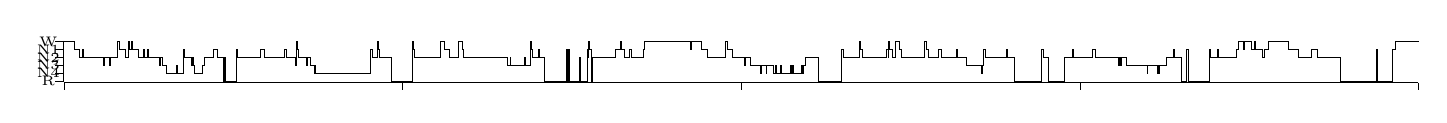
\begin{tikzpicture}[] 
\draw[line width=0.1mm] (0,-0.52)--(17.20, -0.52);
\draw[line width=0.1mm] (0,-0.52)--(0,-0.62);
\draw[line width=0.1mm] (8.60,-0.52)--(8.60,-0.62);
\draw[line width=0.1mm] (17.20,-0.52)--(17.20,-0.62);
\draw[line width=0.1mm] (4.3,-0.52)--(4.3,-0.62);
\draw[line width=0.1mm] (12.9,-0.52)--(12.9,-0.62);
\draw[line width=0.1mm] (-0.01,0.01)--(-0.01,-0.51);
\draw[line width=0.1mm] (-0.01,-0.0)--(-0.11,-0.0);
\draw[line width=0.1mm] (-0.01,-0.1)--(-0.11,-0.1);
\draw[line width=0.1mm] (-0.01,-0.2)--(-0.11,-0.2);
\draw[line width=0.1mm] (-0.01,-0.3)--(-0.11,-0.3);
\draw[line width=0.1mm] (-0.01,-0.4)--(-0.11,-0.4);
\draw[line width=0.1mm] (-0.01,-0.5)--(-0.11,-0.5);
\node at (-0.2,-0.0)   (a) {{\fontsize{2.5}{4}\selectfont W}};
\node at (-0.2,-0.1)   (a) {{\fontsize{2.5}{4}\selectfont N1}};
\node at (-0.2,-0.2)   (a) {{\fontsize{2.5}{4}\selectfont N2}};
\node at (-0.2,-0.3)   (a) {{\fontsize{2.5}{4}\selectfont N3}};
\node at (-0.2,-0.4)   (a) {{\fontsize{2.5}{4}\selectfont N4}};
\node at (-0.2,-0.5)   (a) {{\fontsize{2.5}{4}\selectfont R}};
\draw[line width=0.05mm] (0.00,0.0)--(0.01,0.0)--(0.01,0.0)--(0.02,0.0)--(0.02,0.0)--(0.03,0.0)--(0.03,0.0)--(0.04,0.0)--(0.04,0.0)--(0.05,0.0)--(0.05,0.0)--(0.06,0.0)--(0.06,0.0)--(0.07,0.0)--(0.07,0.0)--(0.08,0.0)--(0.08,0.0)--(0.09,0.0)--(0.09,0.0)--(0.10,0.0)--(0.10,0.0)--(0.11,0.0)--(0.11,0.0)--(0.12,0.0)--(0.12,0.0)--(0.13,0.0)--(0.13,-0.1)--(0.14,-0.1)--(0.14,-0.1)--(0.15,-0.1)--(0.15,-0.1)--(0.16,-0.1)--(0.16,-0.1)--(0.17,-0.1)--(0.17,-0.1)--(0.18,-0.1)--(0.18,-0.1)--(0.19,-0.1)--(0.19,-0.2)--(0.20,-0.2)--(0.20,-0.2)--(0.21,-0.2)--(0.21,-0.2)--(0.22,-0.2)--(0.22,-0.2)--(0.23,-0.2)--(0.23,-0.1)--(0.24,-0.1)--(0.24,-0.2)--(0.25,-0.2)--(0.25,-0.2)--(0.26,-0.2)--(0.26,-0.2)--(0.27,-0.2)--(0.27,-0.2)--(0.28,-0.2)--(0.28,-0.2)--(0.29,-0.2)--(0.29,-0.2)--(0.30,-0.2)--(0.30,-0.2)--(0.31,-0.2)--(0.31,-0.2)--(0.32,-0.2)--(0.32,-0.2)--(0.33,-0.2)--(0.33,-0.2)--(0.34,-0.2)--(0.34,-0.2)--(0.35,-0.2)--(0.35,-0.2)--(0.36,-0.2)--(0.36,-0.2)--(0.37,-0.2)--(0.37,-0.2)--(0.38,-0.2)--(0.38,-0.2)--(0.39,-0.2)--(0.39,-0.2)--(0.40,-0.2)--(0.40,-0.2)--(0.41,-0.2)--(0.41,-0.2)--(0.42,-0.2)--(0.42,-0.2)--(0.43,-0.2)--(0.43,-0.2)--(0.44,-0.2)--(0.44,-0.2)--(0.45,-0.2)--(0.45,-0.2)--(0.46,-0.2)--(0.46,-0.2)--(0.47,-0.2)--(0.47,-0.2)--(0.48,-0.2)--(0.48,-0.2)--(0.49,-0.2)--(0.49,-0.2)--(0.50,-0.2)--(0.50,-0.30000000000000004)--(0.51,-0.30000000000000004)--(0.51,-0.2)--(0.52,-0.2)--(0.52,-0.2)--(0.53,-0.2)--(0.53,-0.2)--(0.54,-0.2)--(0.54,-0.2)--(0.55,-0.2)--(0.55,-0.2)--(0.56,-0.2)--(0.56,-0.2)--(0.57,-0.2)--(0.57,-0.30000000000000004)--(0.58,-0.30000000000000004)--(0.58,-0.2)--(0.59,-0.2)--(0.59,-0.2)--(0.60,-0.2)--(0.60,-0.2)--(0.61,-0.2)--(0.61,-0.2)--(0.62,-0.2)--(0.62,-0.2)--(0.63,-0.2)--(0.63,-0.2)--(0.64,-0.2)--(0.64,-0.2)--(0.65,-0.2)--(0.65,-0.2)--(0.66,-0.2)--(0.66,-0.2)--(0.67,-0.2)--(0.67,0.0)--(0.68,0.0)--(0.68,0.0)--(0.69,0.0)--(0.69,0.0)--(0.70,0.0)--(0.70,-0.1)--(0.71,-0.1)--(0.71,-0.1)--(0.72,-0.1)--(0.72,-0.1)--(0.73,-0.1)--(0.73,-0.1)--(0.74,-0.1)--(0.74,-0.1)--(0.75,-0.1)--(0.75,-0.1)--(0.76,-0.1)--(0.76,-0.1)--(0.77,-0.1)--(0.77,-0.2)--(0.78,-0.2)--(0.78,-0.2)--(0.79,-0.2)--(0.79,-0.2)--(0.80,-0.2)--(0.80,-0.2)--(0.81,-0.2)--(0.81,0.0)--(0.82,0.0)--(0.82,-0.1)--(0.83,-0.1)--(0.83,-0.1)--(0.84,-0.1)--(0.84,-0.1)--(0.85,-0.1)--(0.85,0.0)--(0.86,0.0)--(0.86,0.0)--(0.87,0.0)--(0.87,-0.1)--(0.88,-0.1)--(0.88,-0.1)--(0.89,-0.1)--(0.89,-0.1)--(0.90,-0.1)--(0.90,-0.1)--(0.91,-0.1)--(0.91,-0.1)--(0.92,-0.1)--(0.92,-0.1)--(0.93,-0.1)--(0.93,-0.1)--(0.94,-0.1)--(0.94,-0.2)--(0.95,-0.2)--(0.95,-0.2)--(0.96,-0.2)--(0.96,-0.2)--(0.97,-0.2)--(0.97,-0.2)--(0.98,-0.2)--(0.98,-0.2)--(0.99,-0.2)--(0.99,-0.2)--(1.00,-0.2)--(1.00,-0.2)--(1.01,-0.2)--(1.01,-0.1)--(1.02,-0.1)--(1.02,-0.2)--(1.03,-0.2)--(1.03,-0.2)--(1.04,-0.2)--(1.04,-0.2)--(1.05,-0.2)--(1.05,-0.2)--(1.06,-0.2)--(1.06,-0.1)--(1.07,-0.1)--(1.07,-0.2)--(1.08,-0.2)--(1.08,-0.2)--(1.09,-0.2)--(1.09,-0.2)--(1.10,-0.2)--(1.10,-0.2)--(1.11,-0.2)--(1.11,-0.2)--(1.12,-0.2)--(1.12,-0.2)--(1.13,-0.2)--(1.13,-0.2)--(1.14,-0.2)--(1.14,-0.2)--(1.15,-0.2)--(1.15,-0.2)--(1.16,-0.2)--(1.16,-0.2)--(1.17,-0.2)--(1.17,-0.2)--(1.18,-0.2)--(1.18,-0.2)--(1.19,-0.2)--(1.19,-0.2)--(1.20,-0.2)--(1.20,-0.2)--(1.21,-0.2)--(1.21,-0.30000000000000004)--(1.22,-0.30000000000000004)--(1.22,-0.2)--(1.23,-0.2)--(1.23,-0.2)--(1.24,-0.2)--(1.24,-0.2)--(1.25,-0.2)--(1.25,-0.30000000000000004)--(1.26,-0.30000000000000004)--(1.26,-0.30000000000000004)--(1.27,-0.30000000000000004)--(1.27,-0.30000000000000004)--(1.28,-0.30000000000000004)--(1.28,-0.30000000000000004)--(1.29,-0.30000000000000004)--(1.29,-0.4)--(1.30,-0.4)--(1.30,-0.4)--(1.31,-0.4)--(1.31,-0.4)--(1.32,-0.4)--(1.32,-0.4)--(1.33,-0.4)--(1.33,-0.4)--(1.34,-0.4)--(1.34,-0.4)--(1.35,-0.4)--(1.35,-0.4)--(1.36,-0.4)--(1.36,-0.4)--(1.37,-0.4)--(1.37,-0.4)--(1.38,-0.4)--(1.38,-0.4)--(1.39,-0.4)--(1.39,-0.4)--(1.40,-0.4)--(1.40,-0.4)--(1.41,-0.4)--(1.41,-0.4)--(1.42,-0.4)--(1.42,-0.30000000000000004)--(1.43,-0.30000000000000004)--(1.43,-0.4)--(1.44,-0.4)--(1.44,-0.4)--(1.45,-0.4)--(1.45,-0.4)--(1.46,-0.4)--(1.46,-0.4)--(1.47,-0.4)--(1.47,-0.4)--(1.48,-0.4)--(1.48,-0.4)--(1.49,-0.4)--(1.49,-0.4)--(1.50,-0.4)--(1.50,-0.4)--(1.51,-0.4)--(1.51,-0.1)--(1.52,-0.1)--(1.52,-0.2)--(1.53,-0.2)--(1.53,-0.2)--(1.54,-0.2)--(1.54,-0.2)--(1.55,-0.2)--(1.55,-0.2)--(1.56,-0.2)--(1.56,-0.2)--(1.57,-0.2)--(1.57,-0.2)--(1.58,-0.2)--(1.58,-0.2)--(1.59,-0.2)--(1.59,-0.2)--(1.60,-0.2)--(1.60,-0.2)--(1.61,-0.2)--(1.61,-0.30000000000000004)--(1.62,-0.30000000000000004)--(1.62,-0.2)--(1.63,-0.2)--(1.63,-0.2)--(1.64,-0.2)--(1.64,-0.30000000000000004)--(1.65,-0.30000000000000004)--(1.65,-0.4)--(1.66,-0.4)--(1.66,-0.4)--(1.67,-0.4)--(1.67,-0.4)--(1.68,-0.4)--(1.68,-0.4)--(1.69,-0.4)--(1.69,-0.4)--(1.70,-0.4)--(1.70,-0.4)--(1.71,-0.4)--(1.71,-0.4)--(1.72,-0.4)--(1.72,-0.4)--(1.73,-0.4)--(1.73,-0.4)--(1.74,-0.4)--(1.74,-0.4)--(1.75,-0.4)--(1.75,-0.30000000000000004)--(1.76,-0.30000000000000004)--(1.76,-0.30000000000000004)--(1.77,-0.30000000000000004)--(1.77,-0.30000000000000004)--(1.78,-0.30000000000000004)--(1.78,-0.2)--(1.79,-0.2)--(1.79,-0.2)--(1.80,-0.2)--(1.80,-0.2)--(1.81,-0.2)--(1.81,-0.2)--(1.82,-0.2)--(1.82,-0.2)--(1.83,-0.2)--(1.83,-0.2)--(1.84,-0.2)--(1.84,-0.2)--(1.85,-0.2)--(1.85,-0.2)--(1.86,-0.2)--(1.86,-0.2)--(1.87,-0.2)--(1.87,-0.2)--(1.88,-0.2)--(1.88,-0.2)--(1.89,-0.2)--(1.89,-0.1)--(1.90,-0.1)--(1.90,-0.1)--(1.91,-0.1)--(1.91,-0.1)--(1.92,-0.1)--(1.92,-0.1)--(1.93,-0.1)--(1.93,-0.1)--(1.94,-0.1)--(1.94,-0.2)--(1.95,-0.2)--(1.95,-0.2)--(1.96,-0.2)--(1.96,-0.2)--(1.97,-0.2)--(1.97,-0.2)--(1.98,-0.2)--(1.98,-0.2)--(1.99,-0.2)--(1.99,-0.2)--(2.00,-0.2)--(2.00,-0.2)--(2.01,-0.2)--(2.01,-0.2)--(2.02,-0.2)--(2.02,-0.5)--(2.03,-0.5)--(2.03,-0.2)--(2.04,-0.2)--(2.04,-0.5)--(2.05,-0.5)--(2.05,-0.5)--(2.06,-0.5)--(2.06,-0.5)--(2.07,-0.5)--(2.07,-0.5)--(2.08,-0.5)--(2.08,-0.5)--(2.09,-0.5)--(2.09,-0.5)--(2.10,-0.5)--(2.10,-0.5)--(2.11,-0.5)--(2.11,-0.5)--(2.12,-0.5)--(2.12,-0.5)--(2.13,-0.5)--(2.13,-0.5)--(2.14,-0.5)--(2.14,-0.5)--(2.15,-0.5)--(2.15,-0.5)--(2.16,-0.5)--(2.16,-0.5)--(2.17,-0.5)--(2.17,-0.5)--(2.18,-0.5)--(2.18,-0.1)--(2.19,-0.1)--(2.19,-0.1)--(2.20,-0.1)--(2.20,-0.2)--(2.21,-0.2)--(2.21,-0.2)--(2.22,-0.2)--(2.22,-0.2)--(2.23,-0.2)--(2.23,-0.2)--(2.24,-0.2)--(2.24,-0.2)--(2.25,-0.2)--(2.25,-0.2)--(2.26,-0.2)--(2.26,-0.2)--(2.27,-0.2)--(2.27,-0.2)--(2.28,-0.2)--(2.28,-0.2)--(2.29,-0.2)--(2.29,-0.2)--(2.30,-0.2)--(2.30,-0.2)--(2.31,-0.2)--(2.31,-0.2)--(2.32,-0.2)--(2.32,-0.2)--(2.33,-0.2)--(2.33,-0.2)--(2.34,-0.2)--(2.34,-0.2)--(2.35,-0.2)--(2.35,-0.2)--(2.36,-0.2)--(2.36,-0.2)--(2.37,-0.2)--(2.37,-0.2)--(2.38,-0.2)--(2.38,-0.2)--(2.39,-0.2)--(2.39,-0.2)--(2.40,-0.2)--(2.40,-0.2)--(2.41,-0.2)--(2.41,-0.2)--(2.42,-0.2)--(2.42,-0.2)--(2.43,-0.2)--(2.43,-0.2)--(2.44,-0.2)--(2.44,-0.2)--(2.45,-0.2)--(2.45,-0.2)--(2.46,-0.2)--(2.46,-0.2)--(2.47,-0.2)--(2.47,-0.2)--(2.48,-0.2)--(2.48,-0.2)--(2.49,-0.2)--(2.49,-0.1)--(2.50,-0.1)--(2.50,-0.1)--(2.51,-0.1)--(2.51,-0.1)--(2.52,-0.1)--(2.52,-0.1)--(2.53,-0.1)--(2.53,-0.1)--(2.54,-0.1)--(2.54,-0.2)--(2.55,-0.2)--(2.55,-0.2)--(2.56,-0.2)--(2.56,-0.2)--(2.57,-0.2)--(2.57,-0.2)--(2.58,-0.2)--(2.58,-0.2)--(2.59,-0.2)--(2.59,-0.2)--(2.60,-0.2)--(2.60,-0.2)--(2.61,-0.2)--(2.61,-0.2)--(2.62,-0.2)--(2.62,-0.2)--(2.63,-0.2)--(2.63,-0.2)--(2.64,-0.2)--(2.64,-0.2)--(2.65,-0.2)--(2.65,-0.2)--(2.66,-0.2)--(2.66,-0.2)--(2.67,-0.2)--(2.67,-0.2)--(2.68,-0.2)--(2.68,-0.2)--(2.69,-0.2)--(2.69,-0.2)--(2.70,-0.2)--(2.70,-0.2)--(2.71,-0.2)--(2.71,-0.2)--(2.72,-0.2)--(2.72,-0.2)--(2.73,-0.2)--(2.73,-0.2)--(2.74,-0.2)--(2.74,-0.2)--(2.75,-0.2)--(2.75,-0.2)--(2.76,-0.2)--(2.76,-0.2)--(2.77,-0.2)--(2.77,-0.2)--(2.78,-0.2)--(2.78,-0.2)--(2.79,-0.2)--(2.79,-0.1)--(2.80,-0.1)--(2.80,-0.1)--(2.81,-0.1)--(2.81,-0.1)--(2.82,-0.1)--(2.82,-0.2)--(2.83,-0.2)--(2.83,-0.2)--(2.84,-0.2)--(2.84,-0.2)--(2.85,-0.2)--(2.85,-0.2)--(2.86,-0.2)--(2.86,-0.2)--(2.87,-0.2)--(2.87,-0.2)--(2.88,-0.2)--(2.88,-0.2)--(2.89,-0.2)--(2.89,-0.2)--(2.90,-0.2)--(2.90,-0.2)--(2.91,-0.2)--(2.91,-0.2)--(2.92,-0.2)--(2.92,-0.2)--(2.93,-0.2)--(2.93,-0.2)--(2.94,-0.2)--(2.94,-0.30000000000000004)--(2.95,-0.30000000000000004)--(2.95,0.0)--(2.96,0.0)--(2.96,-0.1)--(2.97,-0.1)--(2.97,-0.2)--(2.98,-0.2)--(2.98,-0.2)--(2.99,-0.2)--(2.99,-0.2)--(3.00,-0.2)--(3.00,-0.2)--(3.01,-0.2)--(3.01,-0.2)--(3.02,-0.2)--(3.02,-0.2)--(3.03,-0.2)--(3.03,-0.2)--(3.04,-0.2)--(3.04,-0.2)--(3.05,-0.2)--(3.05,-0.2)--(3.06,-0.2)--(3.06,-0.2)--(3.07,-0.2)--(3.07,-0.2)--(3.08,-0.2)--(3.08,-0.30000000000000004)--(3.09,-0.30000000000000004)--(3.09,-0.2)--(3.10,-0.2)--(3.10,-0.2)--(3.11,-0.2)--(3.11,-0.2)--(3.12,-0.2)--(3.12,-0.30000000000000004)--(3.13,-0.30000000000000004)--(3.13,-0.30000000000000004)--(3.14,-0.30000000000000004)--(3.14,-0.30000000000000004)--(3.15,-0.30000000000000004)--(3.15,-0.30000000000000004)--(3.16,-0.30000000000000004)--(3.16,-0.30000000000000004)--(3.17,-0.30000000000000004)--(3.17,-0.4)--(3.18,-0.4)--(3.18,-0.30000000000000004)--(3.19,-0.30000000000000004)--(3.19,-0.4)--(3.20,-0.4)--(3.20,-0.4)--(3.21,-0.4)--(3.21,-0.4)--(3.22,-0.4)--(3.22,-0.4)--(3.23,-0.4)--(3.23,-0.4)--(3.24,-0.4)--(3.24,-0.4)--(3.25,-0.4)--(3.25,-0.4)--(3.26,-0.4)--(3.26,-0.4)--(3.27,-0.4)--(3.27,-0.4)--(3.28,-0.4)--(3.28,-0.4)--(3.29,-0.4)--(3.29,-0.4)--(3.30,-0.4)--(3.30,-0.4)--(3.31,-0.4)--(3.31,-0.4)--(3.32,-0.4)--(3.32,-0.4)--(3.33,-0.4)--(3.33,-0.4)--(3.34,-0.4)--(3.34,-0.4)--(3.35,-0.4)--(3.35,-0.4)--(3.36,-0.4)--(3.36,-0.4)--(3.37,-0.4)--(3.37,-0.4)--(3.38,-0.4)--(3.38,-0.4)--(3.39,-0.4)--(3.39,-0.4)--(3.40,-0.4)--(3.40,-0.4)--(3.41,-0.4)--(3.41,-0.4)--(3.42,-0.4)--(3.42,-0.4)--(3.43,-0.4)--(3.43,-0.4)--(3.44,-0.4)--(3.44,-0.4)--(3.45,-0.4)--(3.45,-0.4)--(3.46,-0.4)--(3.46,-0.4)--(3.47,-0.4)--(3.47,-0.4)--(3.48,-0.4)--(3.48,-0.4)--(3.49,-0.4)--(3.49,-0.4)--(3.50,-0.4)--(3.50,-0.4)--(3.51,-0.4)--(3.51,-0.4)--(3.52,-0.4)--(3.52,-0.4)--(3.53,-0.4)--(3.53,-0.4)--(3.54,-0.4)--(3.54,-0.4)--(3.55,-0.4)--(3.55,-0.4)--(3.56,-0.4)--(3.56,-0.4)--(3.57,-0.4)--(3.57,-0.4)--(3.58,-0.4)--(3.58,-0.4)--(3.59,-0.4)--(3.59,-0.4)--(3.60,-0.4)--(3.60,-0.4)--(3.61,-0.4)--(3.61,-0.4)--(3.62,-0.4)--(3.62,-0.4)--(3.63,-0.4)--(3.63,-0.4)--(3.64,-0.4)--(3.64,-0.4)--(3.65,-0.4)--(3.65,-0.4)--(3.66,-0.4)--(3.66,-0.4)--(3.67,-0.4)--(3.67,-0.4)--(3.68,-0.4)--(3.68,-0.4)--(3.69,-0.4)--(3.69,-0.4)--(3.70,-0.4)--(3.70,-0.4)--(3.71,-0.4)--(3.71,-0.4)--(3.72,-0.4)--(3.72,-0.4)--(3.73,-0.4)--(3.73,-0.4)--(3.74,-0.4)--(3.74,-0.4)--(3.75,-0.4)--(3.75,-0.4)--(3.76,-0.4)--(3.76,-0.4)--(3.77,-0.4)--(3.77,-0.4)--(3.78,-0.4)--(3.78,-0.4)--(3.79,-0.4)--(3.79,-0.4)--(3.80,-0.4)--(3.80,-0.4)--(3.81,-0.4)--(3.81,-0.4)--(3.82,-0.4)--(3.82,-0.4)--(3.83,-0.4)--(3.83,-0.4)--(3.84,-0.4)--(3.84,-0.4)--(3.85,-0.4)--(3.85,-0.4)--(3.86,-0.4)--(3.86,-0.4)--(3.87,-0.4)--(3.87,-0.4)--(3.88,-0.4)--(3.88,-0.4)--(3.89,-0.4)--(3.89,-0.1)--(3.90,-0.1)--(3.90,-0.1)--(3.91,-0.1)--(3.91,-0.2)--(3.92,-0.2)--(3.92,-0.2)--(3.93,-0.2)--(3.93,-0.2)--(3.94,-0.2)--(3.94,-0.2)--(3.95,-0.2)--(3.95,-0.2)--(3.96,-0.2)--(3.96,-0.2)--(3.97,-0.2)--(3.97,-0.2)--(3.98,-0.2)--(3.98,0.0)--(3.99,0.0)--(3.99,-0.1)--(4.00,-0.1)--(4.00,-0.2)--(4.01,-0.2)--(4.01,-0.2)--(4.02,-0.2)--(4.02,-0.2)--(4.03,-0.2)--(4.03,-0.2)--(4.04,-0.2)--(4.04,-0.2)--(4.05,-0.2)--(4.05,-0.2)--(4.06,-0.2)--(4.06,-0.2)--(4.07,-0.2)--(4.07,-0.2)--(4.08,-0.2)--(4.08,-0.2)--(4.09,-0.2)--(4.09,-0.2)--(4.10,-0.2)--(4.10,-0.2)--(4.11,-0.2)--(4.11,-0.2)--(4.12,-0.2)--(4.12,-0.2)--(4.13,-0.2)--(4.13,-0.2)--(4.14,-0.2)--(4.14,-0.2)--(4.15,-0.2)--(4.15,-0.5)--(4.16,-0.5)--(4.16,-0.5)--(4.17,-0.5)--(4.17,-0.5)--(4.18,-0.5)--(4.18,-0.5)--(4.19,-0.5)--(4.19,-0.5)--(4.20,-0.5)--(4.20,-0.5)--(4.21,-0.5)--(4.21,-0.5)--(4.22,-0.5)--(4.22,-0.5)--(4.23,-0.5)--(4.23,-0.5)--(4.24,-0.5)--(4.24,-0.5)--(4.25,-0.5)--(4.25,-0.5)--(4.26,-0.5)--(4.26,-0.5)--(4.27,-0.5)--(4.27,-0.5)--(4.28,-0.5)--(4.28,-0.5)--(4.29,-0.5)--(4.29,-0.5)--(4.30,-0.5)--(4.30,-0.5)--(4.31,-0.5)--(4.31,-0.5)--(4.32,-0.5)--(4.32,-0.5)--(4.33,-0.5)--(4.33,-0.5)--(4.34,-0.5)--(4.34,-0.5)--(4.35,-0.5)--(4.35,-0.5)--(4.36,-0.5)--(4.36,-0.5)--(4.37,-0.5)--(4.37,-0.5)--(4.38,-0.5)--(4.38,-0.5)--(4.39,-0.5)--(4.39,-0.5)--(4.40,-0.5)--(4.40,-0.5)--(4.41,-0.5)--(4.41,-0.5)--(4.42,-0.5)--(4.42,0.0)--(4.43,0.0)--(4.43,-0.1)--(4.44,-0.1)--(4.44,-0.2)--(4.45,-0.2)--(4.45,-0.2)--(4.46,-0.2)--(4.46,-0.2)--(4.47,-0.2)--(4.47,-0.2)--(4.48,-0.2)--(4.48,-0.2)--(4.49,-0.2)--(4.49,-0.2)--(4.50,-0.2)--(4.50,-0.2)--(4.51,-0.2)--(4.51,-0.2)--(4.52,-0.2)--(4.52,-0.2)--(4.53,-0.2)--(4.53,-0.2)--(4.54,-0.2)--(4.54,-0.2)--(4.55,-0.2)--(4.55,-0.2)--(4.56,-0.2)--(4.56,-0.2)--(4.57,-0.2)--(4.57,-0.2)--(4.58,-0.2)--(4.58,-0.2)--(4.59,-0.2)--(4.59,-0.2)--(4.60,-0.2)--(4.60,-0.2)--(4.61,-0.2)--(4.61,-0.2)--(4.62,-0.2)--(4.62,-0.2)--(4.63,-0.2)--(4.63,-0.2)--(4.64,-0.2)--(4.64,-0.2)--(4.65,-0.2)--(4.65,-0.2)--(4.66,-0.2)--(4.66,-0.2)--(4.67,-0.2)--(4.67,-0.2)--(4.68,-0.2)--(4.68,-0.2)--(4.69,-0.2)--(4.69,-0.2)--(4.70,-0.2)--(4.70,-0.2)--(4.71,-0.2)--(4.71,-0.2)--(4.72,-0.2)--(4.72,-0.2)--(4.73,-0.2)--(4.73,-0.2)--(4.74,-0.2)--(4.74,-0.2)--(4.75,-0.2)--(4.75,-0.2)--(4.76,-0.2)--(4.76,-0.2)--(4.77,-0.2)--(4.77,0.0)--(4.78,0.0)--(4.78,0.0)--(4.79,0.0)--(4.79,0.0)--(4.80,0.0)--(4.80,0.0)--(4.81,0.0)--(4.81,0.0)--(4.82,0.0)--(4.82,0.0)--(4.83,0.0)--(4.83,-0.1)--(4.84,-0.1)--(4.84,-0.1)--(4.85,-0.1)--(4.85,-0.1)--(4.86,-0.1)--(4.86,-0.1)--(4.87,-0.1)--(4.87,-0.1)--(4.88,-0.1)--(4.88,-0.1)--(4.89,-0.1)--(4.89,-0.2)--(4.90,-0.2)--(4.90,-0.2)--(4.91,-0.2)--(4.91,-0.2)--(4.92,-0.2)--(4.92,-0.2)--(4.93,-0.2)--(4.93,-0.2)--(4.94,-0.2)--(4.94,-0.2)--(4.95,-0.2)--(4.95,-0.2)--(4.96,-0.2)--(4.96,-0.2)--(4.97,-0.2)--(4.97,-0.2)--(4.98,-0.2)--(4.98,-0.2)--(4.99,-0.2)--(4.99,-0.2)--(5.00,-0.2)--(5.00,0.0)--(5.01,0.0)--(5.01,0.0)--(5.02,0.0)--(5.02,0.0)--(5.03,0.0)--(5.03,0.0)--(5.04,0.0)--(5.04,0.0)--(5.05,0.0)--(5.05,-0.1)--(5.06,-0.1)--(5.06,-0.1)--(5.07,-0.1)--(5.07,-0.2)--(5.08,-0.2)--(5.08,-0.2)--(5.09,-0.2)--(5.09,-0.2)--(5.10,-0.2)--(5.10,-0.2)--(5.11,-0.2)--(5.11,-0.2)--(5.12,-0.2)--(5.12,-0.2)--(5.13,-0.2)--(5.13,-0.2)--(5.14,-0.2)--(5.14,-0.2)--(5.15,-0.2)--(5.15,-0.2)--(5.16,-0.2)--(5.16,-0.2)--(5.17,-0.2)--(5.17,-0.2)--(5.18,-0.2)--(5.18,-0.2)--(5.19,-0.2)--(5.19,-0.2)--(5.20,-0.2)--(5.20,-0.2)--(5.21,-0.2)--(5.21,-0.2)--(5.22,-0.2)--(5.22,-0.2)--(5.23,-0.2)--(5.23,-0.2)--(5.24,-0.2)--(5.24,-0.2)--(5.25,-0.2)--(5.25,-0.2)--(5.26,-0.2)--(5.26,-0.2)--(5.27,-0.2)--(5.27,-0.2)--(5.28,-0.2)--(5.28,-0.2)--(5.29,-0.2)--(5.29,-0.2)--(5.30,-0.2)--(5.30,-0.2)--(5.31,-0.2)--(5.31,-0.2)--(5.32,-0.2)--(5.32,-0.2)--(5.33,-0.2)--(5.33,-0.2)--(5.34,-0.2)--(5.34,-0.2)--(5.35,-0.2)--(5.35,-0.2)--(5.36,-0.2)--(5.36,-0.2)--(5.37,-0.2)--(5.37,-0.2)--(5.38,-0.2)--(5.38,-0.2)--(5.39,-0.2)--(5.39,-0.2)--(5.40,-0.2)--(5.40,-0.2)--(5.41,-0.2)--(5.41,-0.2)--(5.42,-0.2)--(5.42,-0.2)--(5.43,-0.2)--(5.43,-0.2)--(5.44,-0.2)--(5.44,-0.2)--(5.45,-0.2)--(5.45,-0.2)--(5.46,-0.2)--(5.46,-0.2)--(5.47,-0.2)--(5.47,-0.2)--(5.48,-0.2)--(5.48,-0.2)--(5.49,-0.2)--(5.49,-0.2)--(5.50,-0.2)--(5.50,-0.2)--(5.51,-0.2)--(5.51,-0.2)--(5.52,-0.2)--(5.52,-0.2)--(5.53,-0.2)--(5.53,-0.2)--(5.54,-0.2)--(5.54,-0.2)--(5.55,-0.2)--(5.55,-0.2)--(5.56,-0.2)--(5.56,-0.2)--(5.57,-0.2)--(5.57,-0.2)--(5.58,-0.2)--(5.58,-0.2)--(5.59,-0.2)--(5.59,-0.2)--(5.60,-0.2)--(5.60,-0.2)--(5.61,-0.2)--(5.61,-0.2)--(5.62,-0.2)--(5.62,-0.2)--(5.63,-0.2)--(5.63,-0.30000000000000004)--(5.64,-0.30000000000000004)--(5.64,-0.30000000000000004)--(5.65,-0.30000000000000004)--(5.65,-0.30000000000000004)--(5.66,-0.30000000000000004)--(5.66,-0.2)--(5.67,-0.2)--(5.67,-0.30000000000000004)--(5.68,-0.30000000000000004)--(5.68,-0.30000000000000004)--(5.69,-0.30000000000000004)--(5.69,-0.30000000000000004)--(5.70,-0.30000000000000004)--(5.70,-0.30000000000000004)--(5.71,-0.30000000000000004)--(5.71,-0.30000000000000004)--(5.72,-0.30000000000000004)--(5.72,-0.30000000000000004)--(5.73,-0.30000000000000004)--(5.73,-0.30000000000000004)--(5.74,-0.30000000000000004)--(5.74,-0.30000000000000004)--(5.75,-0.30000000000000004)--(5.75,-0.30000000000000004)--(5.76,-0.30000000000000004)--(5.76,-0.30000000000000004)--(5.77,-0.30000000000000004)--(5.77,-0.30000000000000004)--(5.78,-0.30000000000000004)--(5.78,-0.30000000000000004)--(5.79,-0.30000000000000004)--(5.79,-0.30000000000000004)--(5.80,-0.30000000000000004)--(5.80,-0.30000000000000004)--(5.81,-0.30000000000000004)--(5.81,-0.30000000000000004)--(5.82,-0.30000000000000004)--(5.82,-0.30000000000000004)--(5.83,-0.30000000000000004)--(5.83,-0.30000000000000004)--(5.84,-0.30000000000000004)--(5.84,-0.2)--(5.85,-0.2)--(5.85,-0.2)--(5.86,-0.2)--(5.86,-0.30000000000000004)--(5.87,-0.30000000000000004)--(5.87,-0.30000000000000004)--(5.88,-0.30000000000000004)--(5.88,-0.30000000000000004)--(5.89,-0.30000000000000004)--(5.89,-0.30000000000000004)--(5.90,-0.30000000000000004)--(5.90,-0.30000000000000004)--(5.91,-0.30000000000000004)--(5.91,-0.30000000000000004)--(5.92,-0.30000000000000004)--(5.92,0.0)--(5.93,0.0)--(5.93,-0.1)--(5.94,-0.1)--(5.94,-0.2)--(5.95,-0.2)--(5.95,-0.2)--(5.96,-0.2)--(5.96,-0.2)--(5.97,-0.2)--(5.97,-0.2)--(5.98,-0.2)--(5.98,-0.2)--(5.99,-0.2)--(5.99,-0.2)--(6.00,-0.2)--(6.00,-0.2)--(6.01,-0.2)--(6.01,-0.2)--(6.02,-0.2)--(6.02,-0.1)--(6.03,-0.1)--(6.03,-0.2)--(6.04,-0.2)--(6.04,-0.2)--(6.05,-0.2)--(6.05,-0.2)--(6.06,-0.2)--(6.06,-0.2)--(6.07,-0.2)--(6.07,-0.2)--(6.08,-0.2)--(6.08,-0.2)--(6.09,-0.2)--(6.09,-0.2)--(6.10,-0.2)--(6.10,-0.5)--(6.11,-0.5)--(6.11,-0.5)--(6.12,-0.5)--(6.12,-0.5)--(6.13,-0.5)--(6.13,-0.5)--(6.14,-0.5)--(6.14,-0.5)--(6.15,-0.5)--(6.15,-0.5)--(6.16,-0.5)--(6.16,-0.5)--(6.17,-0.5)--(6.17,-0.5)--(6.18,-0.5)--(6.18,-0.5)--(6.19,-0.5)--(6.19,-0.5)--(6.20,-0.5)--(6.20,-0.5)--(6.21,-0.5)--(6.21,-0.5)--(6.22,-0.5)--(6.22,-0.5)--(6.23,-0.5)--(6.23,-0.5)--(6.24,-0.5)--(6.24,-0.5)--(6.25,-0.5)--(6.25,-0.5)--(6.26,-0.5)--(6.26,-0.5)--(6.27,-0.5)--(6.27,-0.5)--(6.28,-0.5)--(6.28,-0.5)--(6.29,-0.5)--(6.29,-0.5)--(6.30,-0.5)--(6.30,-0.5)--(6.31,-0.5)--(6.31,-0.5)--(6.32,-0.5)--(6.32,-0.5)--(6.33,-0.5)--(6.33,-0.5)--(6.34,-0.5)--(6.34,-0.5)--(6.35,-0.5)--(6.35,-0.5)--(6.36,-0.5)--(6.36,-0.5)--(6.37,-0.5)--(6.37,-0.5)--(6.38,-0.5)--(6.38,-0.1)--(6.39,-0.1)--(6.39,-0.5)--(6.40,-0.5)--(6.40,-0.1)--(6.41,-0.1)--(6.41,-0.5)--(6.42,-0.5)--(6.42,-0.5)--(6.43,-0.5)--(6.43,-0.5)--(6.44,-0.5)--(6.44,-0.5)--(6.45,-0.5)--(6.45,-0.5)--(6.46,-0.5)--(6.46,-0.5)--(6.47,-0.5)--(6.47,-0.5)--(6.48,-0.5)--(6.48,-0.5)--(6.49,-0.5)--(6.49,-0.5)--(6.50,-0.5)--(6.50,-0.5)--(6.51,-0.5)--(6.51,-0.5)--(6.52,-0.5)--(6.52,-0.5)--(6.53,-0.5)--(6.53,-0.5)--(6.54,-0.5)--(6.54,-0.2)--(6.55,-0.2)--(6.55,-0.5)--(6.56,-0.5)--(6.56,-0.5)--(6.57,-0.5)--(6.57,-0.5)--(6.58,-0.5)--(6.58,-0.5)--(6.59,-0.5)--(6.59,-0.5)--(6.60,-0.5)--(6.60,-0.5)--(6.61,-0.5)--(6.61,-0.5)--(6.62,-0.5)--(6.62,-0.5)--(6.63,-0.5)--(6.63,-0.5)--(6.64,-0.5)--(6.64,-0.1)--(6.65,-0.1)--(6.65,-0.2)--(6.66,-0.2)--(6.66,0.0)--(6.67,0.0)--(6.67,-0.1)--(6.68,-0.1)--(6.68,-0.1)--(6.69,-0.1)--(6.69,-0.5)--(6.70,-0.5)--(6.70,-0.2)--(6.71,-0.2)--(6.71,-0.2)--(6.72,-0.2)--(6.72,-0.2)--(6.73,-0.2)--(6.73,-0.2)--(6.74,-0.2)--(6.74,-0.2)--(6.75,-0.2)--(6.75,-0.2)--(6.76,-0.2)--(6.76,-0.2)--(6.77,-0.2)--(6.77,-0.2)--(6.78,-0.2)--(6.78,-0.2)--(6.79,-0.2)--(6.79,-0.2)--(6.80,-0.2)--(6.80,-0.2)--(6.81,-0.2)--(6.81,-0.2)--(6.82,-0.2)--(6.82,-0.2)--(6.83,-0.2)--(6.83,-0.2)--(6.84,-0.2)--(6.84,-0.2)--(6.85,-0.2)--(6.85,-0.2)--(6.86,-0.2)--(6.86,-0.2)--(6.87,-0.2)--(6.87,-0.2)--(6.88,-0.2)--(6.88,-0.2)--(6.89,-0.2)--(6.89,-0.2)--(6.90,-0.2)--(6.90,-0.2)--(6.91,-0.2)--(6.91,-0.2)--(6.92,-0.2)--(6.92,-0.2)--(6.93,-0.2)--(6.93,-0.2)--(6.94,-0.2)--(6.94,-0.2)--(6.95,-0.2)--(6.95,-0.2)--(6.96,-0.2)--(6.96,-0.2)--(6.97,-0.2)--(6.97,-0.2)--(6.98,-0.2)--(6.98,-0.2)--(6.99,-0.2)--(6.99,-0.2)--(7.00,-0.2)--(7.00,-0.1)--(7.01,-0.1)--(7.01,-0.1)--(7.02,-0.1)--(7.02,-0.1)--(7.03,-0.1)--(7.03,-0.1)--(7.04,-0.1)--(7.04,-0.1)--(7.05,-0.1)--(7.05,-0.1)--(7.06,-0.1)--(7.06,0.0)--(7.07,0.0)--(7.07,-0.1)--(7.08,-0.1)--(7.08,-0.1)--(7.09,-0.1)--(7.09,-0.1)--(7.10,-0.1)--(7.10,-0.1)--(7.11,-0.1)--(7.11,-0.2)--(7.12,-0.2)--(7.12,-0.2)--(7.13,-0.2)--(7.13,-0.2)--(7.14,-0.2)--(7.14,-0.2)--(7.15,-0.2)--(7.15,-0.2)--(7.16,-0.2)--(7.16,-0.2)--(7.17,-0.2)--(7.17,-0.1)--(7.18,-0.1)--(7.18,-0.1)--(7.19,-0.1)--(7.19,-0.1)--(7.20,-0.1)--(7.20,-0.2)--(7.21,-0.2)--(7.21,-0.2)--(7.22,-0.2)--(7.22,-0.2)--(7.23,-0.2)--(7.23,-0.2)--(7.24,-0.2)--(7.24,-0.2)--(7.25,-0.2)--(7.25,-0.2)--(7.26,-0.2)--(7.26,-0.2)--(7.27,-0.2)--(7.27,-0.2)--(7.28,-0.2)--(7.28,-0.2)--(7.29,-0.2)--(7.29,-0.2)--(7.30,-0.2)--(7.30,-0.2)--(7.31,-0.2)--(7.31,-0.2)--(7.32,-0.2)--(7.32,-0.2)--(7.33,-0.2)--(7.33,-0.2)--(7.34,-0.2)--(7.34,-0.2)--(7.35,-0.2)--(7.35,-0.1)--(7.36,-0.1)--(7.36,-0.1)--(7.37,-0.1)--(7.37,0.0)--(7.38,0.0)--(7.38,0.0)--(7.39,0.0)--(7.39,0.0)--(7.40,0.0)--(7.40,0.0)--(7.41,0.0)--(7.41,0.0)--(7.42,0.0)--(7.42,0.0)--(7.43,0.0)--(7.43,0.0)--(7.44,0.0)--(7.44,0.0)--(7.45,0.0)--(7.45,0.0)--(7.46,0.0)--(7.46,0.0)--(7.47,0.0)--(7.47,0.0)--(7.48,0.0)--(7.48,0.0)--(7.49,0.0)--(7.49,0.0)--(7.50,0.0)--(7.50,0.0)--(7.51,0.0)--(7.51,0.0)--(7.52,0.0)--(7.52,0.0)--(7.53,0.0)--(7.53,0.0)--(7.54,0.0)--(7.54,0.0)--(7.55,0.0)--(7.55,0.0)--(7.56,0.0)--(7.56,0.0)--(7.57,0.0)--(7.57,0.0)--(7.58,0.0)--(7.58,0.0)--(7.59,0.0)--(7.59,0.0)--(7.60,0.0)--(7.60,0.0)--(7.61,0.0)--(7.61,0.0)--(7.62,0.0)--(7.62,0.0)--(7.63,0.0)--(7.63,0.0)--(7.64,0.0)--(7.64,0.0)--(7.65,0.0)--(7.65,0.0)--(7.66,0.0)--(7.66,0.0)--(7.67,0.0)--(7.67,0.0)--(7.68,0.0)--(7.68,0.0)--(7.69,0.0)--(7.69,0.0)--(7.70,0.0)--(7.70,0.0)--(7.71,0.0)--(7.71,0.0)--(7.72,0.0)--(7.72,0.0)--(7.73,0.0)--(7.73,0.0)--(7.74,0.0)--(7.74,0.0)--(7.75,0.0)--(7.75,0.0)--(7.76,0.0)--(7.76,0.0)--(7.77,0.0)--(7.77,0.0)--(7.78,0.0)--(7.78,0.0)--(7.79,0.0)--(7.79,0.0)--(7.80,0.0)--(7.80,0.0)--(7.81,0.0)--(7.81,0.0)--(7.82,0.0)--(7.82,0.0)--(7.83,0.0)--(7.83,0.0)--(7.84,0.0)--(7.84,0.0)--(7.85,0.0)--(7.85,0.0)--(7.86,0.0)--(7.86,0.0)--(7.87,0.0)--(7.87,0.0)--(7.88,0.0)--(7.88,0.0)--(7.89,0.0)--(7.89,0.0)--(7.90,0.0)--(7.90,0.0)--(7.91,0.0)--(7.91,0.0)--(7.92,0.0)--(7.92,0.0)--(7.93,0.0)--(7.93,0.0)--(7.94,0.0)--(7.94,0.0)--(7.95,0.0)--(7.95,-0.1)--(7.96,-0.1)--(7.96,0.0)--(7.97,0.0)--(7.97,0.0)--(7.98,0.0)--(7.98,0.0)--(7.99,0.0)--(7.99,0.0)--(8.00,0.0)--(8.00,0.0)--(8.01,0.0)--(8.01,0.0)--(8.02,0.0)--(8.02,0.0)--(8.03,0.0)--(8.03,0.0)--(8.04,0.0)--(8.04,0.0)--(8.05,0.0)--(8.05,0.0)--(8.06,0.0)--(8.06,0.0)--(8.07,0.0)--(8.07,0.0)--(8.08,0.0)--(8.08,0.0)--(8.09,0.0)--(8.09,-0.1)--(8.10,-0.1)--(8.10,-0.1)--(8.11,-0.1)--(8.11,-0.1)--(8.12,-0.1)--(8.12,-0.1)--(8.13,-0.1)--(8.13,-0.1)--(8.14,-0.1)--(8.14,-0.1)--(8.15,-0.1)--(8.15,-0.1)--(8.16,-0.1)--(8.16,-0.1)--(8.17,-0.1)--(8.17,-0.2)--(8.18,-0.2)--(8.18,-0.2)--(8.19,-0.2)--(8.19,-0.2)--(8.20,-0.2)--(8.20,-0.2)--(8.21,-0.2)--(8.21,-0.2)--(8.22,-0.2)--(8.22,-0.2)--(8.23,-0.2)--(8.23,-0.2)--(8.24,-0.2)--(8.24,-0.2)--(8.25,-0.2)--(8.25,-0.2)--(8.26,-0.2)--(8.26,-0.2)--(8.27,-0.2)--(8.27,-0.2)--(8.28,-0.2)--(8.28,-0.2)--(8.29,-0.2)--(8.29,-0.2)--(8.30,-0.2)--(8.30,-0.2)--(8.31,-0.2)--(8.31,-0.2)--(8.32,-0.2)--(8.32,-0.2)--(8.33,-0.2)--(8.33,-0.2)--(8.34,-0.2)--(8.34,-0.2)--(8.35,-0.2)--(8.35,-0.2)--(8.36,-0.2)--(8.36,-0.2)--(8.37,-0.2)--(8.37,-0.2)--(8.38,-0.2)--(8.38,-0.2)--(8.39,-0.2)--(8.39,-0.2)--(8.40,-0.2)--(8.40,0.0)--(8.41,0.0)--(8.41,0.0)--(8.42,0.0)--(8.42,-0.1)--(8.43,-0.1)--(8.43,-0.1)--(8.44,-0.1)--(8.44,-0.1)--(8.45,-0.1)--(8.45,-0.1)--(8.46,-0.1)--(8.46,-0.1)--(8.47,-0.1)--(8.47,-0.1)--(8.48,-0.1)--(8.48,-0.1)--(8.49,-0.1)--(8.49,-0.2)--(8.50,-0.2)--(8.50,-0.2)--(8.51,-0.2)--(8.51,-0.2)--(8.52,-0.2)--(8.52,-0.2)--(8.53,-0.2)--(8.53,-0.2)--(8.54,-0.2)--(8.54,-0.2)--(8.55,-0.2)--(8.55,-0.2)--(8.56,-0.2)--(8.56,-0.2)--(8.57,-0.2)--(8.57,-0.2)--(8.58,-0.2)--(8.58,-0.2)--(8.59,-0.2)--(8.59,-0.2)--(8.60,-0.2)--(8.60,-0.2)--(8.61,-0.2)--(8.61,-0.2)--(8.62,-0.2)--(8.62,-0.2)--(8.63,-0.2)--(8.63,-0.2)--(8.64,-0.2)--(8.64,-0.30000000000000004)--(8.65,-0.30000000000000004)--(8.65,-0.2)--(8.66,-0.2)--(8.66,-0.2)--(8.67,-0.2)--(8.67,-0.2)--(8.68,-0.2)--(8.68,-0.2)--(8.69,-0.2)--(8.69,-0.2)--(8.70,-0.2)--(8.70,-0.2)--(8.71,-0.2)--(8.71,-0.30000000000000004)--(8.72,-0.30000000000000004)--(8.72,-0.30000000000000004)--(8.73,-0.30000000000000004)--(8.73,-0.30000000000000004)--(8.74,-0.30000000000000004)--(8.74,-0.30000000000000004)--(8.75,-0.30000000000000004)--(8.75,-0.30000000000000004)--(8.76,-0.30000000000000004)--(8.76,-0.30000000000000004)--(8.77,-0.30000000000000004)--(8.77,-0.30000000000000004)--(8.78,-0.30000000000000004)--(8.78,-0.30000000000000004)--(8.79,-0.30000000000000004)--(8.79,-0.30000000000000004)--(8.80,-0.30000000000000004)--(8.80,-0.30000000000000004)--(8.81,-0.30000000000000004)--(8.81,-0.30000000000000004)--(8.82,-0.30000000000000004)--(8.82,-0.30000000000000004)--(8.83,-0.30000000000000004)--(8.83,-0.30000000000000004)--(8.84,-0.30000000000000004)--(8.84,-0.4)--(8.85,-0.4)--(8.85,-0.30000000000000004)--(8.86,-0.30000000000000004)--(8.86,-0.30000000000000004)--(8.87,-0.30000000000000004)--(8.87,-0.30000000000000004)--(8.88,-0.30000000000000004)--(8.88,-0.30000000000000004)--(8.89,-0.30000000000000004)--(8.89,-0.30000000000000004)--(8.90,-0.30000000000000004)--(8.90,-0.30000000000000004)--(8.91,-0.30000000000000004)--(8.91,-0.4)--(8.92,-0.4)--(8.92,-0.30000000000000004)--(8.93,-0.30000000000000004)--(8.93,-0.30000000000000004)--(8.94,-0.30000000000000004)--(8.94,-0.30000000000000004)--(8.95,-0.30000000000000004)--(8.95,-0.30000000000000004)--(8.96,-0.30000000000000004)--(8.96,-0.30000000000000004)--(8.97,-0.30000000000000004)--(8.97,-0.30000000000000004)--(8.98,-0.30000000000000004)--(8.98,-0.30000000000000004)--(8.99,-0.30000000000000004)--(8.99,-0.30000000000000004)--(9.00,-0.30000000000000004)--(9.00,-0.30000000000000004)--(9.01,-0.30000000000000004)--(9.01,-0.4)--(9.02,-0.4)--(9.02,-0.4)--(9.03,-0.4)--(9.03,-0.30000000000000004)--(9.04,-0.30000000000000004)--(9.04,-0.4)--(9.05,-0.4)--(9.05,-0.4)--(9.06,-0.4)--(9.06,-0.4)--(9.07,-0.4)--(9.07,-0.4)--(9.08,-0.4)--(9.08,-0.4)--(9.09,-0.4)--(9.09,-0.4)--(9.10,-0.4)--(9.10,-0.30000000000000004)--(9.11,-0.30000000000000004)--(9.11,-0.4)--(9.12,-0.4)--(9.12,-0.4)--(9.13,-0.4)--(9.13,-0.4)--(9.14,-0.4)--(9.14,-0.4)--(9.15,-0.4)--(9.15,-0.4)--(9.16,-0.4)--(9.16,-0.4)--(9.17,-0.4)--(9.17,-0.4)--(9.18,-0.4)--(9.18,-0.4)--(9.19,-0.4)--(9.19,-0.4)--(9.20,-0.4)--(9.20,-0.4)--(9.21,-0.4)--(9.21,-0.4)--(9.22,-0.4)--(9.22,-0.30000000000000004)--(9.23,-0.30000000000000004)--(9.23,-0.4)--(9.24,-0.4)--(9.24,-0.30000000000000004)--(9.25,-0.30000000000000004)--(9.25,-0.30000000000000004)--(9.26,-0.30000000000000004)--(9.26,-0.4)--(9.27,-0.4)--(9.27,-0.4)--(9.28,-0.4)--(9.28,-0.4)--(9.29,-0.4)--(9.29,-0.4)--(9.30,-0.4)--(9.30,-0.4)--(9.31,-0.4)--(9.31,-0.4)--(9.32,-0.4)--(9.32,-0.4)--(9.33,-0.4)--(9.33,-0.4)--(9.34,-0.4)--(9.34,-0.4)--(9.35,-0.4)--(9.35,-0.4)--(9.36,-0.4)--(9.36,-0.30000000000000004)--(9.37,-0.30000000000000004)--(9.37,-0.4)--(9.38,-0.4)--(9.38,-0.30000000000000004)--(9.39,-0.30000000000000004)--(9.39,-0.30000000000000004)--(9.40,-0.30000000000000004)--(9.40,-0.30000000000000004)--(9.41,-0.30000000000000004)--(9.41,-0.2)--(9.42,-0.2)--(9.42,-0.2)--(9.43,-0.2)--(9.43,-0.2)--(9.44,-0.2)--(9.44,-0.2)--(9.45,-0.2)--(9.45,-0.2)--(9.46,-0.2)--(9.46,-0.2)--(9.47,-0.2)--(9.47,-0.2)--(9.48,-0.2)--(9.48,-0.2)--(9.49,-0.2)--(9.49,-0.2)--(9.50,-0.2)--(9.50,-0.2)--(9.51,-0.2)--(9.51,-0.2)--(9.52,-0.2)--(9.52,-0.2)--(9.53,-0.2)--(9.53,-0.2)--(9.54,-0.2)--(9.54,-0.2)--(9.55,-0.2)--(9.55,-0.2)--(9.56,-0.2)--(9.56,-0.2)--(9.57,-0.2)--(9.57,-0.2)--(9.58,-0.2)--(9.58,-0.5)--(9.59,-0.5)--(9.59,-0.5)--(9.60,-0.5)--(9.60,-0.5)--(9.61,-0.5)--(9.61,-0.5)--(9.62,-0.5)--(9.62,-0.5)--(9.63,-0.5)--(9.63,-0.5)--(9.64,-0.5)--(9.64,-0.5)--(9.65,-0.5)--(9.65,-0.5)--(9.66,-0.5)--(9.66,-0.5)--(9.67,-0.5)--(9.67,-0.5)--(9.68,-0.5)--(9.68,-0.5)--(9.69,-0.5)--(9.69,-0.5)--(9.70,-0.5)--(9.70,-0.5)--(9.71,-0.5)--(9.71,-0.5)--(9.72,-0.5)--(9.72,-0.5)--(9.73,-0.5)--(9.73,-0.5)--(9.74,-0.5)--(9.74,-0.5)--(9.75,-0.5)--(9.75,-0.5)--(9.76,-0.5)--(9.76,-0.5)--(9.77,-0.5)--(9.77,-0.5)--(9.78,-0.5)--(9.78,-0.5)--(9.79,-0.5)--(9.79,-0.5)--(9.80,-0.5)--(9.80,-0.5)--(9.81,-0.5)--(9.81,-0.5)--(9.82,-0.5)--(9.82,-0.5)--(9.83,-0.5)--(9.83,-0.5)--(9.84,-0.5)--(9.84,-0.5)--(9.85,-0.5)--(9.85,-0.5)--(9.86,-0.5)--(9.86,-0.5)--(9.87,-0.5)--(9.87,-0.1)--(9.88,-0.1)--(9.88,-0.1)--(9.89,-0.1)--(9.89,-0.1)--(9.90,-0.1)--(9.90,-0.2)--(9.91,-0.2)--(9.91,-0.2)--(9.92,-0.2)--(9.92,-0.2)--(9.93,-0.2)--(9.93,-0.2)--(9.94,-0.2)--(9.94,-0.2)--(9.95,-0.2)--(9.95,-0.2)--(9.96,-0.2)--(9.96,-0.2)--(9.97,-0.2)--(9.97,-0.2)--(9.98,-0.2)--(9.98,-0.2)--(9.99,-0.2)--(9.99,-0.2)--(10.00,-0.2)--(10.00,-0.2)--(10.01,-0.2)--(10.01,-0.2)--(10.02,-0.2)--(10.02,-0.2)--(10.03,-0.2)--(10.03,-0.2)--(10.04,-0.2)--(10.04,-0.2)--(10.05,-0.2)--(10.05,-0.2)--(10.06,-0.2)--(10.06,-0.2)--(10.07,-0.2)--(10.07,-0.2)--(10.08,-0.2)--(10.08,-0.2)--(10.09,-0.2)--(10.09,-0.2)--(10.10,-0.2)--(10.10,0.0)--(10.11,0.0)--(10.11,-0.1)--(10.12,-0.1)--(10.12,-0.1)--(10.13,-0.1)--(10.13,-0.2)--(10.14,-0.2)--(10.14,-0.2)--(10.15,-0.2)--(10.15,-0.2)--(10.16,-0.2)--(10.16,-0.2)--(10.17,-0.2)--(10.17,-0.2)--(10.18,-0.2)--(10.18,-0.2)--(10.19,-0.2)--(10.19,-0.2)--(10.20,-0.2)--(10.20,-0.2)--(10.21,-0.2)--(10.21,-0.2)--(10.22,-0.2)--(10.22,-0.2)--(10.23,-0.2)--(10.23,-0.2)--(10.24,-0.2)--(10.24,-0.2)--(10.25,-0.2)--(10.25,-0.2)--(10.26,-0.2)--(10.26,-0.2)--(10.27,-0.2)--(10.27,-0.2)--(10.28,-0.2)--(10.28,-0.2)--(10.29,-0.2)--(10.29,-0.2)--(10.30,-0.2)--(10.30,-0.2)--(10.31,-0.2)--(10.31,-0.2)--(10.32,-0.2)--(10.32,-0.2)--(10.33,-0.2)--(10.33,-0.2)--(10.34,-0.2)--(10.34,-0.2)--(10.35,-0.2)--(10.35,-0.2)--(10.36,-0.2)--(10.36,-0.2)--(10.37,-0.2)--(10.37,-0.2)--(10.38,-0.2)--(10.38,-0.2)--(10.39,-0.2)--(10.39,-0.2)--(10.40,-0.2)--(10.40,-0.2)--(10.41,-0.2)--(10.41,-0.2)--(10.42,-0.2)--(10.42,-0.2)--(10.43,-0.2)--(10.43,-0.2)--(10.44,-0.2)--(10.44,-0.1)--(10.45,-0.1)--(10.45,-0.1)--(10.46,-0.1)--(10.46,-0.2)--(10.47,-0.2)--(10.47,0.0)--(10.48,0.0)--(10.48,-0.1)--(10.49,-0.1)--(10.49,-0.1)--(10.50,-0.1)--(10.50,-0.1)--(10.51,-0.1)--(10.51,-0.2)--(10.52,-0.2)--(10.52,-0.2)--(10.53,-0.2)--(10.53,-0.2)--(10.54,-0.2)--(10.54,-0.2)--(10.55,-0.2)--(10.55,0.0)--(10.56,0.0)--(10.56,0.0)--(10.57,0.0)--(10.57,0.0)--(10.58,0.0)--(10.58,0.0)--(10.59,0.0)--(10.59,0.0)--(10.60,0.0)--(10.60,-0.1)--(10.61,-0.1)--(10.61,-0.1)--(10.62,-0.1)--(10.62,-0.1)--(10.63,-0.1)--(10.63,-0.2)--(10.64,-0.2)--(10.64,-0.2)--(10.65,-0.2)--(10.65,-0.2)--(10.66,-0.2)--(10.66,-0.2)--(10.67,-0.2)--(10.67,-0.2)--(10.68,-0.2)--(10.68,-0.2)--(10.69,-0.2)--(10.69,-0.2)--(10.70,-0.2)--(10.70,-0.2)--(10.71,-0.2)--(10.71,-0.2)--(10.72,-0.2)--(10.72,-0.2)--(10.73,-0.2)--(10.73,-0.2)--(10.74,-0.2)--(10.74,-0.2)--(10.75,-0.2)--(10.75,-0.2)--(10.76,-0.2)--(10.76,-0.2)--(10.77,-0.2)--(10.77,-0.2)--(10.78,-0.2)--(10.78,-0.2)--(10.79,-0.2)--(10.79,-0.2)--(10.80,-0.2)--(10.80,-0.2)--(10.81,-0.2)--(10.81,-0.2)--(10.82,-0.2)--(10.82,-0.2)--(10.83,-0.2)--(10.83,-0.2)--(10.84,-0.2)--(10.84,-0.2)--(10.85,-0.2)--(10.85,-0.2)--(10.86,-0.2)--(10.86,-0.2)--(10.87,-0.2)--(10.87,-0.2)--(10.88,-0.2)--(10.88,-0.2)--(10.89,-0.2)--(10.89,-0.2)--(10.90,-0.2)--(10.90,-0.2)--(10.91,-0.2)--(10.91,-0.2)--(10.92,-0.2)--(10.92,0.0)--(10.93,0.0)--(10.93,0.0)--(10.94,0.0)--(10.94,0.0)--(10.95,0.0)--(10.95,-0.1)--(10.96,-0.1)--(10.96,-0.1)--(10.97,-0.1)--(10.97,-0.2)--(10.98,-0.2)--(10.98,-0.2)--(10.99,-0.2)--(10.99,-0.2)--(11.00,-0.2)--(11.00,-0.2)--(11.01,-0.2)--(11.01,-0.2)--(11.02,-0.2)--(11.02,-0.2)--(11.03,-0.2)--(11.03,-0.2)--(11.04,-0.2)--(11.04,-0.2)--(11.05,-0.2)--(11.05,-0.2)--(11.06,-0.2)--(11.06,-0.2)--(11.07,-0.2)--(11.07,-0.2)--(11.08,-0.2)--(11.08,-0.2)--(11.09,-0.2)--(11.09,-0.2)--(11.10,-0.2)--(11.10,-0.1)--(11.11,-0.1)--(11.11,-0.1)--(11.12,-0.1)--(11.12,-0.1)--(11.13,-0.1)--(11.13,-0.1)--(11.14,-0.1)--(11.14,-0.2)--(11.15,-0.2)--(11.15,-0.2)--(11.16,-0.2)--(11.16,-0.2)--(11.17,-0.2)--(11.17,-0.2)--(11.18,-0.2)--(11.18,-0.2)--(11.19,-0.2)--(11.19,-0.2)--(11.20,-0.2)--(11.20,-0.2)--(11.21,-0.2)--(11.21,-0.2)--(11.22,-0.2)--(11.22,-0.2)--(11.23,-0.2)--(11.23,-0.2)--(11.24,-0.2)--(11.24,-0.2)--(11.25,-0.2)--(11.25,-0.2)--(11.26,-0.2)--(11.26,-0.2)--(11.27,-0.2)--(11.27,-0.2)--(11.28,-0.2)--(11.28,-0.2)--(11.29,-0.2)--(11.29,-0.2)--(11.30,-0.2)--(11.30,-0.2)--(11.31,-0.2)--(11.31,-0.2)--(11.32,-0.2)--(11.32,-0.2)--(11.33,-0.2)--(11.33,-0.1)--(11.34,-0.1)--(11.34,-0.2)--(11.35,-0.2)--(11.35,-0.2)--(11.36,-0.2)--(11.36,-0.2)--(11.37,-0.2)--(11.37,-0.2)--(11.38,-0.2)--(11.38,-0.2)--(11.39,-0.2)--(11.39,-0.2)--(11.40,-0.2)--(11.40,-0.2)--(11.41,-0.2)--(11.41,-0.2)--(11.42,-0.2)--(11.42,-0.2)--(11.43,-0.2)--(11.43,-0.2)--(11.44,-0.2)--(11.44,-0.2)--(11.45,-0.2)--(11.45,-0.2)--(11.46,-0.2)--(11.46,-0.30000000000000004)--(11.47,-0.30000000000000004)--(11.47,-0.30000000000000004)--(11.48,-0.30000000000000004)--(11.48,-0.30000000000000004)--(11.49,-0.30000000000000004)--(11.49,-0.30000000000000004)--(11.50,-0.30000000000000004)--(11.50,-0.30000000000000004)--(11.51,-0.30000000000000004)--(11.51,-0.30000000000000004)--(11.52,-0.30000000000000004)--(11.52,-0.30000000000000004)--(11.53,-0.30000000000000004)--(11.53,-0.30000000000000004)--(11.54,-0.30000000000000004)--(11.54,-0.30000000000000004)--(11.55,-0.30000000000000004)--(11.55,-0.30000000000000004)--(11.56,-0.30000000000000004)--(11.56,-0.30000000000000004)--(11.57,-0.30000000000000004)--(11.57,-0.30000000000000004)--(11.58,-0.30000000000000004)--(11.58,-0.30000000000000004)--(11.59,-0.30000000000000004)--(11.59,-0.30000000000000004)--(11.60,-0.30000000000000004)--(11.60,-0.30000000000000004)--(11.61,-0.30000000000000004)--(11.61,-0.30000000000000004)--(11.62,-0.30000000000000004)--(11.62,-0.30000000000000004)--(11.63,-0.30000000000000004)--(11.63,-0.30000000000000004)--(11.64,-0.30000000000000004)--(11.64,-0.30000000000000004)--(11.65,-0.30000000000000004)--(11.65,-0.4)--(11.66,-0.4)--(11.66,-0.30000000000000004)--(11.67,-0.30000000000000004)--(11.67,-0.1)--(11.68,-0.1)--(11.68,-0.1)--(11.69,-0.1)--(11.69,-0.1)--(11.70,-0.1)--(11.70,-0.2)--(11.71,-0.2)--(11.71,-0.2)--(11.72,-0.2)--(11.72,-0.2)--(11.73,-0.2)--(11.73,-0.2)--(11.74,-0.2)--(11.74,-0.2)--(11.75,-0.2)--(11.75,-0.2)--(11.76,-0.2)--(11.76,-0.2)--(11.77,-0.2)--(11.77,-0.2)--(11.78,-0.2)--(11.78,-0.2)--(11.79,-0.2)--(11.79,-0.2)--(11.80,-0.2)--(11.80,-0.2)--(11.81,-0.2)--(11.81,-0.2)--(11.82,-0.2)--(11.82,-0.2)--(11.83,-0.2)--(11.83,-0.2)--(11.84,-0.2)--(11.84,-0.2)--(11.85,-0.2)--(11.85,-0.2)--(11.86,-0.2)--(11.86,-0.2)--(11.87,-0.2)--(11.87,-0.2)--(11.88,-0.2)--(11.88,-0.2)--(11.89,-0.2)--(11.89,-0.2)--(11.90,-0.2)--(11.90,-0.2)--(11.91,-0.2)--(11.91,-0.2)--(11.92,-0.2)--(11.92,-0.2)--(11.93,-0.2)--(11.93,-0.2)--(11.94,-0.2)--(11.94,-0.2)--(11.95,-0.2)--(11.95,-0.2)--(11.96,-0.2)--(11.96,-0.1)--(11.97,-0.1)--(11.97,-0.1)--(11.98,-0.1)--(11.98,-0.2)--(11.99,-0.2)--(11.99,-0.2)--(12.00,-0.2)--(12.00,-0.2)--(12.01,-0.2)--(12.01,-0.2)--(12.02,-0.2)--(12.02,-0.2)--(12.03,-0.2)--(12.03,-0.2)--(12.04,-0.2)--(12.04,-0.2)--(12.05,-0.2)--(12.05,-0.2)--(12.06,-0.2)--(12.06,-0.2)--(12.07,-0.2)--(12.07,-0.5)--(12.08,-0.5)--(12.08,-0.5)--(12.09,-0.5)--(12.09,-0.5)--(12.10,-0.5)--(12.10,-0.5)--(12.11,-0.5)--(12.11,-0.5)--(12.12,-0.5)--(12.12,-0.5)--(12.13,-0.5)--(12.13,-0.5)--(12.14,-0.5)--(12.14,-0.5)--(12.15,-0.5)--(12.15,-0.5)--(12.16,-0.5)--(12.16,-0.5)--(12.17,-0.5)--(12.17,-0.5)--(12.18,-0.5)--(12.18,-0.5)--(12.19,-0.5)--(12.19,-0.5)--(12.20,-0.5)--(12.20,-0.5)--(12.21,-0.5)--(12.21,-0.5)--(12.22,-0.5)--(12.22,-0.5)--(12.23,-0.5)--(12.23,-0.5)--(12.24,-0.5)--(12.24,-0.5)--(12.25,-0.5)--(12.25,-0.5)--(12.26,-0.5)--(12.26,-0.5)--(12.27,-0.5)--(12.27,-0.5)--(12.28,-0.5)--(12.28,-0.5)--(12.29,-0.5)--(12.29,-0.5)--(12.30,-0.5)--(12.30,-0.5)--(12.31,-0.5)--(12.31,-0.5)--(12.32,-0.5)--(12.32,-0.5)--(12.33,-0.5)--(12.33,-0.5)--(12.34,-0.5)--(12.34,-0.5)--(12.35,-0.5)--(12.35,-0.5)--(12.36,-0.5)--(12.36,-0.5)--(12.37,-0.5)--(12.37,-0.5)--(12.38,-0.5)--(12.38,-0.5)--(12.39,-0.5)--(12.39,-0.5)--(12.40,-0.5)--(12.40,-0.5)--(12.41,-0.5)--(12.41,-0.1)--(12.42,-0.1)--(12.42,-0.1)--(12.43,-0.1)--(12.43,-0.1)--(12.44,-0.1)--(12.44,-0.2)--(12.45,-0.2)--(12.45,-0.2)--(12.46,-0.2)--(12.46,-0.2)--(12.47,-0.2)--(12.47,-0.2)--(12.48,-0.2)--(12.48,-0.2)--(12.49,-0.2)--(12.49,-0.2)--(12.50,-0.2)--(12.50,-0.5)--(12.51,-0.5)--(12.51,-0.5)--(12.52,-0.5)--(12.52,-0.5)--(12.53,-0.5)--(12.53,-0.5)--(12.54,-0.5)--(12.54,-0.5)--(12.55,-0.5)--(12.55,-0.5)--(12.56,-0.5)--(12.56,-0.5)--(12.57,-0.5)--(12.57,-0.5)--(12.58,-0.5)--(12.58,-0.5)--(12.59,-0.5)--(12.59,-0.5)--(12.60,-0.5)--(12.60,-0.5)--(12.61,-0.5)--(12.61,-0.5)--(12.62,-0.5)--(12.62,-0.5)--(12.63,-0.5)--(12.63,-0.5)--(12.64,-0.5)--(12.64,-0.5)--(12.65,-0.5)--(12.65,-0.5)--(12.66,-0.5)--(12.66,-0.5)--(12.67,-0.5)--(12.67,-0.5)--(12.68,-0.5)--(12.68,-0.5)--(12.69,-0.5)--(12.69,-0.5)--(12.70,-0.5)--(12.70,-0.2)--(12.71,-0.2)--(12.71,-0.2)--(12.72,-0.2)--(12.72,-0.2)--(12.73,-0.2)--(12.73,-0.2)--(12.74,-0.2)--(12.74,-0.2)--(12.75,-0.2)--(12.75,-0.2)--(12.76,-0.2)--(12.76,-0.2)--(12.77,-0.2)--(12.77,-0.2)--(12.78,-0.2)--(12.78,-0.2)--(12.79,-0.2)--(12.79,-0.2)--(12.80,-0.2)--(12.80,-0.1)--(12.81,-0.1)--(12.81,-0.1)--(12.82,-0.1)--(12.82,-0.2)--(12.83,-0.2)--(12.83,-0.2)--(12.84,-0.2)--(12.84,-0.2)--(12.85,-0.2)--(12.85,-0.2)--(12.86,-0.2)--(12.86,-0.2)--(12.87,-0.2)--(12.87,-0.2)--(12.88,-0.2)--(12.88,-0.2)--(12.89,-0.2)--(12.89,-0.2)--(12.90,-0.2)--(12.90,-0.2)--(12.91,-0.2)--(12.91,-0.2)--(12.92,-0.2)--(12.92,-0.2)--(12.93,-0.2)--(12.93,-0.2)--(12.94,-0.2)--(12.94,-0.2)--(12.95,-0.2)--(12.95,-0.2)--(12.96,-0.2)--(12.96,-0.2)--(12.97,-0.2)--(12.97,-0.2)--(12.98,-0.2)--(12.98,-0.2)--(12.99,-0.2)--(12.99,-0.2)--(13.00,-0.2)--(13.00,-0.2)--(13.01,-0.2)--(13.01,-0.2)--(13.02,-0.2)--(13.02,-0.2)--(13.03,-0.2)--(13.03,-0.2)--(13.04,-0.2)--(13.04,-0.2)--(13.05,-0.2)--(13.05,-0.1)--(13.06,-0.1)--(13.06,-0.1)--(13.07,-0.1)--(13.07,-0.1)--(13.08,-0.1)--(13.08,-0.1)--(13.09,-0.1)--(13.09,-0.1)--(13.10,-0.1)--(13.10,-0.2)--(13.11,-0.2)--(13.11,-0.2)--(13.12,-0.2)--(13.12,-0.2)--(13.13,-0.2)--(13.13,-0.2)--(13.14,-0.2)--(13.14,-0.2)--(13.15,-0.2)--(13.15,-0.2)--(13.16,-0.2)--(13.16,-0.2)--(13.17,-0.2)--(13.17,-0.2)--(13.18,-0.2)--(13.18,-0.2)--(13.19,-0.2)--(13.19,-0.2)--(13.20,-0.2)--(13.20,-0.2)--(13.21,-0.2)--(13.21,-0.2)--(13.22,-0.2)--(13.22,-0.2)--(13.23,-0.2)--(13.23,-0.2)--(13.24,-0.2)--(13.24,-0.2)--(13.25,-0.2)--(13.25,-0.2)--(13.26,-0.2)--(13.26,-0.2)--(13.27,-0.2)--(13.27,-0.2)--(13.28,-0.2)--(13.28,-0.2)--(13.29,-0.2)--(13.29,-0.2)--(13.30,-0.2)--(13.30,-0.2)--(13.31,-0.2)--(13.31,-0.2)--(13.32,-0.2)--(13.32,-0.2)--(13.33,-0.2)--(13.33,-0.2)--(13.34,-0.2)--(13.34,-0.2)--(13.35,-0.2)--(13.35,-0.2)--(13.36,-0.2)--(13.36,-0.2)--(13.37,-0.2)--(13.37,-0.2)--(13.38,-0.2)--(13.38,-0.2)--(13.39,-0.2)--(13.39,-0.30000000000000004)--(13.40,-0.30000000000000004)--(13.40,-0.2)--(13.41,-0.2)--(13.41,-0.30000000000000004)--(13.42,-0.30000000000000004)--(13.42,-0.2)--(13.43,-0.2)--(13.43,-0.2)--(13.44,-0.2)--(13.44,-0.2)--(13.45,-0.2)--(13.45,-0.2)--(13.46,-0.2)--(13.46,-0.2)--(13.47,-0.2)--(13.47,-0.2)--(13.48,-0.2)--(13.48,-0.2)--(13.49,-0.2)--(13.49,-0.30000000000000004)--(13.50,-0.30000000000000004)--(13.50,-0.30000000000000004)--(13.51,-0.30000000000000004)--(13.51,-0.30000000000000004)--(13.52,-0.30000000000000004)--(13.52,-0.30000000000000004)--(13.53,-0.30000000000000004)--(13.53,-0.30000000000000004)--(13.54,-0.30000000000000004)--(13.54,-0.30000000000000004)--(13.55,-0.30000000000000004)--(13.55,-0.30000000000000004)--(13.56,-0.30000000000000004)--(13.56,-0.30000000000000004)--(13.57,-0.30000000000000004)--(13.57,-0.30000000000000004)--(13.58,-0.30000000000000004)--(13.58,-0.30000000000000004)--(13.59,-0.30000000000000004)--(13.59,-0.30000000000000004)--(13.60,-0.30000000000000004)--(13.60,-0.30000000000000004)--(13.61,-0.30000000000000004)--(13.61,-0.30000000000000004)--(13.62,-0.30000000000000004)--(13.62,-0.30000000000000004)--(13.63,-0.30000000000000004)--(13.63,-0.30000000000000004)--(13.64,-0.30000000000000004)--(13.64,-0.30000000000000004)--(13.65,-0.30000000000000004)--(13.65,-0.30000000000000004)--(13.66,-0.30000000000000004)--(13.66,-0.30000000000000004)--(13.67,-0.30000000000000004)--(13.67,-0.30000000000000004)--(13.68,-0.30000000000000004)--(13.68,-0.30000000000000004)--(13.69,-0.30000000000000004)--(13.69,-0.30000000000000004)--(13.70,-0.30000000000000004)--(13.70,-0.30000000000000004)--(13.71,-0.30000000000000004)--(13.71,-0.30000000000000004)--(13.72,-0.30000000000000004)--(13.72,-0.30000000000000004)--(13.73,-0.30000000000000004)--(13.73,-0.30000000000000004)--(13.74,-0.30000000000000004)--(13.74,-0.30000000000000004)--(13.75,-0.30000000000000004)--(13.75,-0.4)--(13.76,-0.4)--(13.76,-0.30000000000000004)--(13.77,-0.30000000000000004)--(13.77,-0.30000000000000004)--(13.78,-0.30000000000000004)--(13.78,-0.30000000000000004)--(13.79,-0.30000000000000004)--(13.79,-0.30000000000000004)--(13.80,-0.30000000000000004)--(13.80,-0.30000000000000004)--(13.81,-0.30000000000000004)--(13.81,-0.30000000000000004)--(13.82,-0.30000000000000004)--(13.82,-0.30000000000000004)--(13.83,-0.30000000000000004)--(13.83,-0.30000000000000004)--(13.84,-0.30000000000000004)--(13.84,-0.30000000000000004)--(13.85,-0.30000000000000004)--(13.85,-0.30000000000000004)--(13.86,-0.30000000000000004)--(13.86,-0.30000000000000004)--(13.87,-0.30000000000000004)--(13.87,-0.30000000000000004)--(13.88,-0.30000000000000004)--(13.88,-0.4)--(13.89,-0.4)--(13.89,-0.30000000000000004)--(13.90,-0.30000000000000004)--(13.90,-0.4)--(13.91,-0.4)--(13.91,-0.30000000000000004)--(13.92,-0.30000000000000004)--(13.92,-0.30000000000000004)--(13.93,-0.30000000000000004)--(13.93,-0.30000000000000004)--(13.94,-0.30000000000000004)--(13.94,-0.30000000000000004)--(13.95,-0.30000000000000004)--(13.95,-0.30000000000000004)--(13.96,-0.30000000000000004)--(13.96,-0.30000000000000004)--(13.97,-0.30000000000000004)--(13.97,-0.30000000000000004)--(13.98,-0.30000000000000004)--(13.98,-0.30000000000000004)--(13.99,-0.30000000000000004)--(13.99,-0.30000000000000004)--(14.00,-0.30000000000000004)--(14.00,-0.2)--(14.01,-0.2)--(14.01,-0.2)--(14.02,-0.2)--(14.02,-0.2)--(14.03,-0.2)--(14.03,-0.2)--(14.04,-0.2)--(14.04,-0.2)--(14.05,-0.2)--(14.05,-0.2)--(14.06,-0.2)--(14.06,-0.2)--(14.07,-0.2)--(14.07,-0.2)--(14.08,-0.2)--(14.08,-0.2)--(14.09,-0.2)--(14.09,-0.1)--(14.10,-0.1)--(14.10,-0.2)--(14.11,-0.2)--(14.11,-0.2)--(14.12,-0.2)--(14.12,-0.2)--(14.13,-0.2)--(14.13,-0.2)--(14.14,-0.2)--(14.14,-0.2)--(14.15,-0.2)--(14.15,-0.2)--(14.16,-0.2)--(14.16,-0.2)--(14.17,-0.2)--(14.17,-0.2)--(14.18,-0.2)--(14.18,-0.2)--(14.19,-0.2)--(14.19,-0.5)--(14.20,-0.5)--(14.20,-0.5)--(14.21,-0.5)--(14.21,-0.5)--(14.22,-0.5)--(14.22,-0.5)--(14.23,-0.5)--(14.23,-0.5)--(14.24,-0.5)--(14.24,-0.5)--(14.25,-0.5)--(14.25,-0.1)--(14.26,-0.1)--(14.26,-0.1)--(14.27,-0.1)--(14.27,-0.5)--(14.28,-0.5)--(14.28,-0.5)--(14.29,-0.5)--(14.29,-0.5)--(14.30,-0.5)--(14.30,-0.5)--(14.31,-0.5)--(14.31,-0.5)--(14.32,-0.5)--(14.32,-0.5)--(14.33,-0.5)--(14.33,-0.5)--(14.34,-0.5)--(14.34,-0.5)--(14.35,-0.5)--(14.35,-0.5)--(14.36,-0.5)--(14.36,-0.5)--(14.37,-0.5)--(14.37,-0.5)--(14.38,-0.5)--(14.38,-0.5)--(14.39,-0.5)--(14.39,-0.5)--(14.40,-0.5)--(14.40,-0.5)--(14.41,-0.5)--(14.41,-0.5)--(14.42,-0.5)--(14.42,-0.5)--(14.43,-0.5)--(14.43,-0.5)--(14.44,-0.5)--(14.44,-0.5)--(14.45,-0.5)--(14.45,-0.5)--(14.46,-0.5)--(14.46,-0.5)--(14.47,-0.5)--(14.47,-0.5)--(14.48,-0.5)--(14.48,-0.5)--(14.49,-0.5)--(14.49,-0.5)--(14.50,-0.5)--(14.50,-0.5)--(14.51,-0.5)--(14.51,-0.5)--(14.52,-0.5)--(14.52,-0.5)--(14.53,-0.5)--(14.53,-0.5)--(14.54,-0.5)--(14.54,-0.1)--(14.55,-0.1)--(14.55,-0.1)--(14.56,-0.1)--(14.56,-0.2)--(14.57,-0.2)--(14.57,-0.2)--(14.58,-0.2)--(14.58,-0.2)--(14.59,-0.2)--(14.59,-0.2)--(14.60,-0.2)--(14.60,-0.2)--(14.61,-0.2)--(14.61,-0.2)--(14.62,-0.2)--(14.62,-0.2)--(14.63,-0.2)--(14.63,-0.2)--(14.64,-0.2)--(14.64,-0.2)--(14.65,-0.2)--(14.65,-0.1)--(14.66,-0.1)--(14.66,-0.2)--(14.67,-0.2)--(14.67,-0.2)--(14.68,-0.2)--(14.68,-0.2)--(14.69,-0.2)--(14.69,-0.2)--(14.70,-0.2)--(14.70,-0.2)--(14.71,-0.2)--(14.71,-0.2)--(14.72,-0.2)--(14.72,-0.2)--(14.73,-0.2)--(14.73,-0.2)--(14.74,-0.2)--(14.74,-0.2)--(14.75,-0.2)--(14.75,-0.2)--(14.76,-0.2)--(14.76,-0.2)--(14.77,-0.2)--(14.77,-0.2)--(14.78,-0.2)--(14.78,-0.2)--(14.79,-0.2)--(14.79,-0.2)--(14.80,-0.2)--(14.80,-0.2)--(14.81,-0.2)--(14.81,-0.2)--(14.82,-0.2)--(14.82,-0.2)--(14.83,-0.2)--(14.83,-0.2)--(14.84,-0.2)--(14.84,-0.2)--(14.85,-0.2)--(14.85,-0.2)--(14.86,-0.2)--(14.86,-0.2)--(14.87,-0.2)--(14.87,-0.2)--(14.88,-0.2)--(14.88,-0.2)--(14.89,-0.2)--(14.89,-0.1)--(14.90,-0.1)--(14.90,-0.1)--(14.91,-0.1)--(14.91,0.0)--(14.92,0.0)--(14.92,0.0)--(14.93,0.0)--(14.93,0.0)--(14.94,0.0)--(14.94,0.0)--(14.95,0.0)--(14.95,0.0)--(14.96,0.0)--(14.96,0.0)--(14.97,0.0)--(14.97,0.0)--(14.98,0.0)--(14.98,-0.1)--(14.99,-0.1)--(14.99,0.0)--(15.00,0.0)--(15.00,0.0)--(15.01,0.0)--(15.01,0.0)--(15.02,0.0)--(15.02,0.0)--(15.03,0.0)--(15.03,0.0)--(15.04,0.0)--(15.04,0.0)--(15.05,0.0)--(15.05,0.0)--(15.06,0.0)--(15.06,0.0)--(15.07,0.0)--(15.07,0.0)--(15.08,0.0)--(15.08,-0.1)--(15.09,-0.1)--(15.09,-0.1)--(15.10,-0.1)--(15.10,-0.1)--(15.11,-0.1)--(15.11,0.0)--(15.12,0.0)--(15.12,-0.1)--(15.13,-0.1)--(15.13,-0.1)--(15.14,-0.1)--(15.14,-0.1)--(15.15,-0.1)--(15.15,-0.1)--(15.16,-0.1)--(15.16,-0.1)--(15.17,-0.1)--(15.17,-0.1)--(15.18,-0.1)--(15.18,-0.1)--(15.19,-0.1)--(15.19,-0.1)--(15.20,-0.1)--(15.20,-0.1)--(15.21,-0.1)--(15.21,-0.2)--(15.22,-0.2)--(15.22,-0.2)--(15.23,-0.2)--(15.23,-0.2)--(15.24,-0.2)--(15.24,-0.1)--(15.25,-0.1)--(15.25,-0.1)--(15.26,-0.1)--(15.26,-0.1)--(15.27,-0.1)--(15.27,-0.1)--(15.28,-0.1)--(15.28,-0.1)--(15.29,-0.1)--(15.29,0.0)--(15.30,0.0)--(15.30,0.0)--(15.31,0.0)--(15.31,0.0)--(15.32,0.0)--(15.32,0.0)--(15.33,0.0)--(15.33,0.0)--(15.34,0.0)--(15.34,0.0)--(15.35,0.0)--(15.35,0.0)--(15.36,0.0)--(15.36,0.0)--(15.37,0.0)--(15.37,0.0)--(15.38,0.0)--(15.38,0.0)--(15.39,0.0)--(15.39,0.0)--(15.40,0.0)--(15.40,0.0)--(15.41,0.0)--(15.41,0.0)--(15.42,0.0)--(15.42,0.0)--(15.43,0.0)--(15.43,0.0)--(15.44,0.0)--(15.44,0.0)--(15.45,0.0)--(15.45,0.0)--(15.46,0.0)--(15.46,0.0)--(15.47,0.0)--(15.47,0.0)--(15.48,0.0)--(15.48,0.0)--(15.49,0.0)--(15.49,0.0)--(15.50,0.0)--(15.50,0.0)--(15.51,0.0)--(15.51,0.0)--(15.52,0.0)--(15.52,0.0)--(15.53,0.0)--(15.53,0.0)--(15.54,0.0)--(15.54,-0.1)--(15.55,-0.1)--(15.55,-0.1)--(15.56,-0.1)--(15.56,-0.1)--(15.57,-0.1)--(15.57,-0.1)--(15.58,-0.1)--(15.58,-0.1)--(15.59,-0.1)--(15.59,-0.1)--(15.60,-0.1)--(15.60,-0.1)--(15.61,-0.1)--(15.61,-0.1)--(15.62,-0.1)--(15.62,-0.1)--(15.63,-0.1)--(15.63,-0.1)--(15.64,-0.1)--(15.64,-0.1)--(15.65,-0.1)--(15.65,-0.1)--(15.66,-0.1)--(15.66,-0.1)--(15.67,-0.1)--(15.67,-0.2)--(15.68,-0.2)--(15.68,-0.2)--(15.69,-0.2)--(15.69,-0.2)--(15.70,-0.2)--(15.70,-0.2)--(15.71,-0.2)--(15.71,-0.2)--(15.72,-0.2)--(15.72,-0.2)--(15.73,-0.2)--(15.73,-0.2)--(15.74,-0.2)--(15.74,-0.2)--(15.75,-0.2)--(15.75,-0.2)--(15.76,-0.2)--(15.76,-0.2)--(15.77,-0.2)--(15.77,-0.2)--(15.78,-0.2)--(15.78,-0.2)--(15.79,-0.2)--(15.79,-0.2)--(15.80,-0.2)--(15.80,-0.2)--(15.81,-0.2)--(15.81,-0.2)--(15.82,-0.2)--(15.82,-0.2)--(15.83,-0.2)--(15.83,-0.2)--(15.84,-0.2)--(15.84,-0.1)--(15.85,-0.1)--(15.85,-0.1)--(15.86,-0.1)--(15.86,-0.1)--(15.87,-0.1)--(15.87,-0.1)--(15.88,-0.1)--(15.88,-0.1)--(15.89,-0.1)--(15.89,-0.1)--(15.90,-0.1)--(15.90,-0.1)--(15.91,-0.1)--(15.91,-0.2)--(15.92,-0.2)--(15.92,-0.2)--(15.93,-0.2)--(15.93,-0.2)--(15.94,-0.2)--(15.94,-0.2)--(15.95,-0.2)--(15.95,-0.2)--(15.96,-0.2)--(15.96,-0.2)--(15.97,-0.2)--(15.97,-0.2)--(15.98,-0.2)--(15.98,-0.2)--(15.99,-0.2)--(15.99,-0.2)--(16.00,-0.2)--(16.00,-0.2)--(16.01,-0.2)--(16.01,-0.2)--(16.02,-0.2)--(16.02,-0.2)--(16.03,-0.2)--(16.03,-0.2)--(16.04,-0.2)--(16.04,-0.2)--(16.05,-0.2)--(16.05,-0.2)--(16.06,-0.2)--(16.06,-0.2)--(16.07,-0.2)--(16.07,-0.2)--(16.08,-0.2)--(16.08,-0.2)--(16.09,-0.2)--(16.09,-0.2)--(16.10,-0.2)--(16.10,-0.2)--(16.11,-0.2)--(16.11,-0.2)--(16.12,-0.2)--(16.12,-0.2)--(16.13,-0.2)--(16.13,-0.2)--(16.14,-0.2)--(16.14,-0.2)--(16.15,-0.2)--(16.15,-0.2)--(16.16,-0.2)--(16.16,-0.2)--(16.17,-0.2)--(16.17,-0.2)--(16.18,-0.2)--(16.18,-0.2)--(16.19,-0.2)--(16.19,-0.2)--(16.20,-0.2)--(16.20,-0.5)--(16.21,-0.5)--(16.21,-0.5)--(16.22,-0.5)--(16.22,-0.5)--(16.23,-0.5)--(16.23,-0.5)--(16.24,-0.5)--(16.24,-0.5)--(16.25,-0.5)--(16.25,-0.5)--(16.26,-0.5)--(16.26,-0.5)--(16.27,-0.5)--(16.27,-0.5)--(16.28,-0.5)--(16.28,-0.5)--(16.29,-0.5)--(16.29,-0.5)--(16.30,-0.5)--(16.30,-0.5)--(16.31,-0.5)--(16.31,-0.5)--(16.32,-0.5)--(16.32,-0.5)--(16.33,-0.5)--(16.33,-0.5)--(16.34,-0.5)--(16.34,-0.5)--(16.35,-0.5)--(16.35,-0.5)--(16.36,-0.5)--(16.36,-0.5)--(16.37,-0.5)--(16.37,-0.5)--(16.38,-0.5)--(16.38,-0.5)--(16.39,-0.5)--(16.39,-0.5)--(16.40,-0.5)--(16.40,-0.5)--(16.41,-0.5)--(16.41,-0.5)--(16.42,-0.5)--(16.42,-0.5)--(16.43,-0.5)--(16.43,-0.5)--(16.44,-0.5)--(16.44,-0.5)--(16.45,-0.5)--(16.45,-0.5)--(16.46,-0.5)--(16.46,-0.5)--(16.47,-0.5)--(16.47,-0.5)--(16.48,-0.5)--(16.48,-0.5)--(16.49,-0.5)--(16.49,-0.5)--(16.50,-0.5)--(16.50,-0.5)--(16.51,-0.5)--(16.51,-0.5)--(16.52,-0.5)--(16.52,-0.5)--(16.53,-0.5)--(16.53,-0.5)--(16.54,-0.5)--(16.54,-0.5)--(16.55,-0.5)--(16.55,-0.5)--(16.56,-0.5)--(16.56,-0.5)--(16.57,-0.5)--(16.57,-0.5)--(16.58,-0.5)--(16.58,-0.5)--(16.59,-0.5)--(16.59,-0.5)--(16.60,-0.5)--(16.60,-0.5)--(16.61,-0.5)--(16.61,-0.5)--(16.62,-0.5)--(16.62,-0.5)--(16.63,-0.5)--(16.63,-0.5)--(16.64,-0.5)--(16.64,-0.5)--(16.65,-0.5)--(16.65,-0.5)--(16.66,-0.5)--(16.66,-0.1)--(16.67,-0.1)--(16.67,-0.5)--(16.68,-0.5)--(16.68,-0.5)--(16.69,-0.5)--(16.69,-0.5)--(16.70,-0.5)--(16.70,-0.5)--(16.71,-0.5)--(16.71,-0.5)--(16.72,-0.5)--(16.72,-0.5)--(16.73,-0.5)--(16.73,-0.5)--(16.74,-0.5)--(16.74,-0.5)--(16.75,-0.5)--(16.75,-0.5)--(16.76,-0.5)--(16.76,-0.5)--(16.77,-0.5)--(16.77,-0.5)--(16.78,-0.5)--(16.78,-0.5)--(16.79,-0.5)--(16.79,-0.5)--(16.80,-0.5)--(16.80,-0.5)--(16.81,-0.5)--(16.81,-0.5)--(16.82,-0.5)--(16.82,-0.5)--(16.83,-0.5)--(16.83,-0.5)--(16.84,-0.5)--(16.84,-0.5)--(16.85,-0.5)--(16.85,-0.5)--(16.86,-0.5)--(16.86,-0.5)--(16.87,-0.5)--(16.87,-0.1)--(16.88,-0.1)--(16.88,-0.1)--(16.89,-0.1)--(16.89,-0.1)--(16.90,-0.1)--(16.90,-0.1)--(16.91,-0.1)--(16.91,0.0)--(16.92,0.0)--(16.92,0.0)--(16.93,0.0)--(16.93,0.0)--(16.94,0.0)--(16.94,0.0)--(16.95,0.0)--(16.95,0.0)--(16.96,0.0)--(16.96,0.0)--(16.97,0.0)--(16.97,0.0)--(16.98,0.0)--(16.98,0.0)--(16.99,0.0)--(16.99,0.0)--(17.00,0.0)--(17.00,0.0)--(17.01,0.0)--(17.01,0.0)--(17.02,0.0)--(17.02,0.0)--(17.03,0.0)--(17.03,0.0)--(17.04,0.0)--(17.04,0.0)--(17.05,0.0)--(17.05,0.0)--(17.06,0.0)--(17.06,0.0)--(17.07,0.0)--(17.07,0.0)--(17.08,0.0)--(17.08,0.0)--(17.09,0.0)--(17.09,0.0)--(17.10,0.0)--(17.10,0.0)--(17.11,0.0)--(17.11,0.0)--(17.12,0.0)--(17.12,0.0)--(17.13,0.0)--(17.13,0.0)--(17.14,0.0)--(17.14,0.0)--(17.15,0.0)--(17.15,0.0)--(17.16,0.0)--(17.16,0.0)--(17.17,0.0)--(17.17,0.0)--(17.18,0.0)--(17.18,0.0)--(17.19,0.0)--(17.19,0.0)--(17.20,0.0)--(17.20,0.0);
\end{tikzpicture}
\caption{}
\label{fig_hyp_2}
\end{subfigure}

\begin{subfigure}{1\textwidth}
\centering
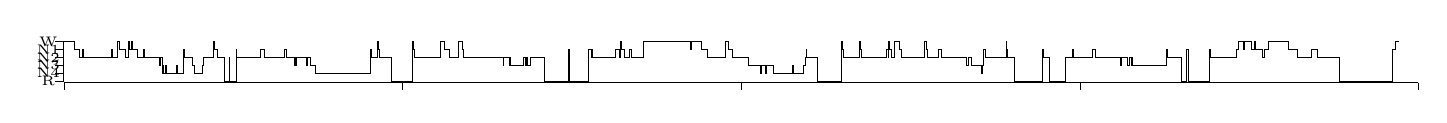
\begin{tikzpicture}[] 
\draw[line width=0.1mm] (0,-0.52)--(17.20, -0.52);

%\node at (0,-0.8)   (a) {$t_{0}$};
%\node at (4.3,-0.8)   (a) {$t_{430}$};
%\node at (8.60,-0.8)   (a) {$t_{860}$};
%\node at (12.90,-0.8)   (a) {$t_{1290}$};
%\node at (16.90,-0.8)   (a) {$t_{1720}$};
%\node at (8.60,-1.2)   (a) {time $\left[ s \right]$};

\draw[line width=0.1mm] (0,-0.52)--(0,-0.62);
\draw[line width=0.1mm] (8.60,-0.52)--(8.60,-0.62);
\draw[line width=0.1mm] (17.20,-0.52)--(17.20,-0.62);
\draw[line width=0.1mm] (4.3,-0.52)--(4.3,-0.62);
\draw[line width=0.1mm] (12.9,-0.52)--(12.9,-0.62);

\draw[line width=0.1mm] (-0.01,0.01)--(-0.01,-0.51);
\draw[line width=0.1mm] (-0.01,-0.0)--(-0.11,-0.0);
\draw[line width=0.1mm] (-0.01,-0.1)--(-0.11,-0.1);
\draw[line width=0.1mm] (-0.01,-0.2)--(-0.11,-0.2);
\draw[line width=0.1mm] (-0.01,-0.3)--(-0.11,-0.3);
\draw[line width=0.1mm] (-0.01,-0.4)--(-0.11,-0.4);
\draw[line width=0.1mm] (-0.01,-0.5)--(-0.11,-0.5);
\node at (-0.2,-0.0)   (a) {{\fontsize{2.5}{4}\selectfont W}};
\node at (-0.2,-0.1)   (a) {{\fontsize{2.5}{4}\selectfont N1}};
\node at (-0.2,-0.2)   (a) {{\fontsize{2.5}{4}\selectfont N2}};
\node at (-0.2,-0.3)   (a) {{\fontsize{2.5}{4}\selectfont N3}};
\node at (-0.2,-0.4)   (a) {{\fontsize{2.5}{4}\selectfont N4}};
\node at (-0.2,-0.5)   (a) {{\fontsize{2.5}{4}\selectfont R}};
\draw[line width=0.05mm] (0.00,0.0)--(0.01,0.0)--(0.01,0.0)--(0.02,0.0)--(0.02,0.0)--(0.03,0.0)--(0.03,0.0)--(0.04,0.0)--(0.04,0.0)--(0.05,0.0)--(0.05,0.0)--(0.06,0.0)--(0.06,0.0)--(0.07,0.0)--(0.07,0.0)--(0.08,0.0)--(0.08,0.0)--(0.09,0.0)--(0.09,0.0)--(0.10,0.0)--(0.10,0.0)--(0.11,0.0)--(0.11,0.0)--(0.12,0.0)--(0.12,0.0)--(0.13,0.0)--(0.13,-0.1)--(0.14,-0.1)--(0.14,-0.1)--(0.15,-0.1)--(0.15,-0.1)--(0.16,-0.1)--(0.16,-0.1)--(0.17,-0.1)--(0.17,-0.1)--(0.18,-0.1)--(0.18,-0.1)--(0.19,-0.1)--(0.19,-0.2)--(0.20,-0.2)--(0.20,-0.2)--(0.21,-0.2)--(0.21,-0.2)--(0.22,-0.2)--(0.22,-0.2)--(0.23,-0.2)--(0.23,-0.1)--(0.24,-0.1)--(0.24,-0.2)--(0.25,-0.2)--(0.25,-0.2)--(0.26,-0.2)--(0.26,-0.2)--(0.27,-0.2)--(0.27,-0.2)--(0.28,-0.2)--(0.28,-0.2)--(0.29,-0.2)--(0.29,-0.2)--(0.30,-0.2)--(0.30,-0.2)--(0.31,-0.2)--(0.31,-0.2)--(0.32,-0.2)--(0.32,-0.2)--(0.33,-0.2)--(0.33,-0.2)--(0.34,-0.2)--(0.34,-0.2)--(0.35,-0.2)--(0.35,-0.2)--(0.36,-0.2)--(0.36,-0.2)--(0.37,-0.2)--(0.37,-0.2)--(0.38,-0.2)--(0.38,-0.2)--(0.39,-0.2)--(0.39,-0.2)--(0.40,-0.2)--(0.40,-0.2)--(0.41,-0.2)--(0.41,-0.2)--(0.42,-0.2)--(0.42,-0.2)--(0.43,-0.2)--(0.43,-0.2)--(0.44,-0.2)--(0.44,-0.2)--(0.45,-0.2)--(0.45,-0.2)--(0.46,-0.2)--(0.46,-0.2)--(0.47,-0.2)--(0.47,-0.2)--(0.48,-0.2)--(0.48,-0.2)--(0.49,-0.2)--(0.49,-0.2)--(0.50,-0.2)--(0.50,-0.2)--(0.51,-0.2)--(0.51,-0.2)--(0.52,-0.2)--(0.52,-0.2)--(0.53,-0.2)--(0.53,-0.2)--(0.54,-0.2)--(0.54,-0.2)--(0.55,-0.2)--(0.55,-0.2)--(0.56,-0.2)--(0.56,-0.2)--(0.57,-0.2)--(0.57,-0.2)--(0.58,-0.2)--(0.58,-0.2)--(0.59,-0.2)--(0.59,-0.2)--(0.60,-0.2)--(0.60,-0.1)--(0.61,-0.1)--(0.61,-0.2)--(0.62,-0.2)--(0.62,-0.2)--(0.63,-0.2)--(0.63,-0.2)--(0.64,-0.2)--(0.64,-0.2)--(0.65,-0.2)--(0.65,-0.2)--(0.66,-0.2)--(0.66,-0.2)--(0.67,-0.2)--(0.67,-0.2)--(0.68,-0.2)--(0.68,0.0)--(0.69,0.0)--(0.69,0.0)--(0.70,0.0)--(0.70,-0.1)--(0.71,-0.1)--(0.71,-0.1)--(0.72,-0.1)--(0.72,-0.1)--(0.73,-0.1)--(0.73,-0.1)--(0.74,-0.1)--(0.74,-0.1)--(0.75,-0.1)--(0.75,-0.1)--(0.76,-0.1)--(0.76,-0.1)--(0.77,-0.1)--(0.77,-0.2)--(0.78,-0.2)--(0.78,-0.2)--(0.79,-0.2)--(0.79,-0.2)--(0.80,-0.2)--(0.80,-0.2)--(0.81,-0.2)--(0.81,0.0)--(0.82,0.0)--(0.82,-0.1)--(0.83,-0.1)--(0.83,-0.1)--(0.84,-0.1)--(0.84,-0.1)--(0.85,-0.1)--(0.85,0.0)--(0.86,0.0)--(0.86,0.0)--(0.87,0.0)--(0.87,-0.1)--(0.88,-0.1)--(0.88,-0.1)--(0.89,-0.1)--(0.89,-0.1)--(0.90,-0.1)--(0.90,-0.1)--(0.91,-0.1)--(0.91,-0.1)--(0.92,-0.1)--(0.92,-0.1)--(0.93,-0.1)--(0.93,-0.2)--(0.94,-0.2)--(0.94,-0.2)--(0.95,-0.2)--(0.95,-0.2)--(0.96,-0.2)--(0.96,-0.2)--(0.97,-0.2)--(0.97,-0.2)--(0.98,-0.2)--(0.98,-0.2)--(0.99,-0.2)--(0.99,-0.2)--(1.00,-0.2)--(1.00,-0.2)--(1.01,-0.2)--(1.01,-0.1)--(1.02,-0.1)--(1.02,-0.2)--(1.03,-0.2)--(1.03,-0.2)--(1.04,-0.2)--(1.04,-0.2)--(1.05,-0.2)--(1.05,-0.2)--(1.06,-0.2)--(1.06,-0.2)--(1.07,-0.2)--(1.07,-0.2)--(1.08,-0.2)--(1.08,-0.2)--(1.09,-0.2)--(1.09,-0.2)--(1.10,-0.2)--(1.10,-0.2)--(1.11,-0.2)--(1.11,-0.2)--(1.12,-0.2)--(1.12,-0.2)--(1.13,-0.2)--(1.13,-0.2)--(1.14,-0.2)--(1.14,-0.2)--(1.15,-0.2)--(1.15,-0.2)--(1.16,-0.2)--(1.16,-0.2)--(1.17,-0.2)--(1.17,-0.2)--(1.18,-0.2)--(1.18,-0.2)--(1.19,-0.2)--(1.19,-0.2)--(1.20,-0.2)--(1.20,-0.2)--(1.21,-0.2)--(1.21,-0.30000000000000004)--(1.22,-0.30000000000000004)--(1.22,-0.2)--(1.23,-0.2)--(1.23,-0.2)--(1.24,-0.2)--(1.24,-0.4)--(1.25,-0.4)--(1.25,-0.30000000000000004)--(1.26,-0.30000000000000004)--(1.26,-0.4)--(1.27,-0.4)--(1.27,-0.4)--(1.28,-0.4)--(1.28,-0.30000000000000004)--(1.29,-0.30000000000000004)--(1.29,-0.4)--(1.30,-0.4)--(1.30,-0.4)--(1.31,-0.4)--(1.31,-0.4)--(1.32,-0.4)--(1.32,-0.4)--(1.33,-0.4)--(1.33,-0.4)--(1.34,-0.4)--(1.34,-0.4)--(1.35,-0.4)--(1.35,-0.4)--(1.36,-0.4)--(1.36,-0.4)--(1.37,-0.4)--(1.37,-0.4)--(1.38,-0.4)--(1.38,-0.4)--(1.39,-0.4)--(1.39,-0.4)--(1.40,-0.4)--(1.40,-0.4)--(1.41,-0.4)--(1.41,-0.4)--(1.42,-0.4)--(1.42,-0.30000000000000004)--(1.43,-0.30000000000000004)--(1.43,-0.4)--(1.44,-0.4)--(1.44,-0.4)--(1.45,-0.4)--(1.45,-0.4)--(1.46,-0.4)--(1.46,-0.4)--(1.47,-0.4)--(1.47,-0.4)--(1.48,-0.4)--(1.48,-0.4)--(1.49,-0.4)--(1.49,-0.4)--(1.50,-0.4)--(1.50,-0.4)--(1.51,-0.4)--(1.51,-0.1)--(1.52,-0.1)--(1.52,-0.2)--(1.53,-0.2)--(1.53,-0.2)--(1.54,-0.2)--(1.54,-0.2)--(1.55,-0.2)--(1.55,-0.2)--(1.56,-0.2)--(1.56,-0.2)--(1.57,-0.2)--(1.57,-0.2)--(1.58,-0.2)--(1.58,-0.2)--(1.59,-0.2)--(1.59,-0.2)--(1.60,-0.2)--(1.60,-0.2)--(1.61,-0.2)--(1.61,-0.2)--(1.62,-0.2)--(1.62,-0.30000000000000004)--(1.63,-0.30000000000000004)--(1.63,-0.30000000000000004)--(1.64,-0.30000000000000004)--(1.64,-0.30000000000000004)--(1.65,-0.30000000000000004)--(1.65,-0.4)--(1.66,-0.4)--(1.66,-0.4)--(1.67,-0.4)--(1.67,-0.4)--(1.68,-0.4)--(1.68,-0.4)--(1.69,-0.4)--(1.69,-0.4)--(1.70,-0.4)--(1.70,-0.4)--(1.71,-0.4)--(1.71,-0.4)--(1.72,-0.4)--(1.72,-0.4)--(1.73,-0.4)--(1.73,-0.4)--(1.74,-0.4)--(1.74,-0.4)--(1.75,-0.4)--(1.75,-0.30000000000000004)--(1.76,-0.30000000000000004)--(1.76,-0.2)--(1.77,-0.2)--(1.77,-0.2)--(1.78,-0.2)--(1.78,-0.2)--(1.79,-0.2)--(1.79,-0.2)--(1.80,-0.2)--(1.80,-0.2)--(1.81,-0.2)--(1.81,-0.2)--(1.82,-0.2)--(1.82,-0.2)--(1.83,-0.2)--(1.83,-0.2)--(1.84,-0.2)--(1.84,-0.2)--(1.85,-0.2)--(1.85,-0.2)--(1.86,-0.2)--(1.86,-0.2)--(1.87,-0.2)--(1.87,-0.2)--(1.88,-0.2)--(1.88,-0.2)--(1.89,-0.2)--(1.89,0.0)--(1.90,0.0)--(1.90,-0.1)--(1.91,-0.1)--(1.91,-0.1)--(1.92,-0.1)--(1.92,-0.1)--(1.93,-0.1)--(1.93,-0.1)--(1.94,-0.1)--(1.94,-0.2)--(1.95,-0.2)--(1.95,-0.2)--(1.96,-0.2)--(1.96,-0.2)--(1.97,-0.2)--(1.97,-0.2)--(1.98,-0.2)--(1.98,-0.2)--(1.99,-0.2)--(1.99,-0.2)--(2.00,-0.2)--(2.00,-0.2)--(2.01,-0.2)--(2.01,-0.2)--(2.02,-0.2)--(2.02,-0.2)--(2.03,-0.2)--(2.03,-0.5)--(2.04,-0.5)--(2.04,-0.5)--(2.05,-0.5)--(2.05,-0.5)--(2.06,-0.5)--(2.06,-0.5)--(2.07,-0.5)--(2.07,-0.5)--(2.08,-0.5)--(2.08,-0.5)--(2.09,-0.5)--(2.09,-0.2)--(2.10,-0.2)--(2.10,-0.5)--(2.11,-0.5)--(2.11,-0.5)--(2.12,-0.5)--(2.12,-0.5)--(2.13,-0.5)--(2.13,-0.5)--(2.14,-0.5)--(2.14,-0.5)--(2.15,-0.5)--(2.15,-0.5)--(2.16,-0.5)--(2.16,-0.5)--(2.17,-0.5)--(2.17,-0.5)--(2.18,-0.5)--(2.18,-0.1)--(2.19,-0.1)--(2.19,-0.2)--(2.20,-0.2)--(2.20,-0.2)--(2.21,-0.2)--(2.21,-0.2)--(2.22,-0.2)--(2.22,-0.2)--(2.23,-0.2)--(2.23,-0.2)--(2.24,-0.2)--(2.24,-0.2)--(2.25,-0.2)--(2.25,-0.2)--(2.26,-0.2)--(2.26,-0.2)--(2.27,-0.2)--(2.27,-0.2)--(2.28,-0.2)--(2.28,-0.2)--(2.29,-0.2)--(2.29,-0.2)--(2.30,-0.2)--(2.30,-0.2)--(2.31,-0.2)--(2.31,-0.2)--(2.32,-0.2)--(2.32,-0.2)--(2.33,-0.2)--(2.33,-0.2)--(2.34,-0.2)--(2.34,-0.2)--(2.35,-0.2)--(2.35,-0.2)--(2.36,-0.2)--(2.36,-0.2)--(2.37,-0.2)--(2.37,-0.2)--(2.38,-0.2)--(2.38,-0.2)--(2.39,-0.2)--(2.39,-0.2)--(2.40,-0.2)--(2.40,-0.2)--(2.41,-0.2)--(2.41,-0.2)--(2.42,-0.2)--(2.42,-0.2)--(2.43,-0.2)--(2.43,-0.2)--(2.44,-0.2)--(2.44,-0.2)--(2.45,-0.2)--(2.45,-0.2)--(2.46,-0.2)--(2.46,-0.2)--(2.47,-0.2)--(2.47,-0.2)--(2.48,-0.2)--(2.48,-0.2)--(2.49,-0.2)--(2.49,-0.1)--(2.50,-0.1)--(2.50,-0.1)--(2.51,-0.1)--(2.51,-0.1)--(2.52,-0.1)--(2.52,-0.1)--(2.53,-0.1)--(2.53,-0.1)--(2.54,-0.1)--(2.54,-0.2)--(2.55,-0.2)--(2.55,-0.2)--(2.56,-0.2)--(2.56,-0.2)--(2.57,-0.2)--(2.57,-0.2)--(2.58,-0.2)--(2.58,-0.2)--(2.59,-0.2)--(2.59,-0.2)--(2.60,-0.2)--(2.60,-0.2)--(2.61,-0.2)--(2.61,-0.2)--(2.62,-0.2)--(2.62,-0.2)--(2.63,-0.2)--(2.63,-0.2)--(2.64,-0.2)--(2.64,-0.2)--(2.65,-0.2)--(2.65,-0.2)--(2.66,-0.2)--(2.66,-0.2)--(2.67,-0.2)--(2.67,-0.2)--(2.68,-0.2)--(2.68,-0.2)--(2.69,-0.2)--(2.69,-0.2)--(2.70,-0.2)--(2.70,-0.2)--(2.71,-0.2)--(2.71,-0.2)--(2.72,-0.2)--(2.72,-0.2)--(2.73,-0.2)--(2.73,-0.2)--(2.74,-0.2)--(2.74,-0.2)--(2.75,-0.2)--(2.75,-0.2)--(2.76,-0.2)--(2.76,-0.2)--(2.77,-0.2)--(2.77,-0.2)--(2.78,-0.2)--(2.78,-0.2)--(2.79,-0.2)--(2.79,-0.1)--(2.80,-0.1)--(2.80,-0.1)--(2.81,-0.1)--(2.81,-0.1)--(2.82,-0.1)--(2.82,-0.2)--(2.83,-0.2)--(2.83,-0.2)--(2.84,-0.2)--(2.84,-0.2)--(2.85,-0.2)--(2.85,-0.2)--(2.86,-0.2)--(2.86,-0.2)--(2.87,-0.2)--(2.87,-0.2)--(2.88,-0.2)--(2.88,-0.2)--(2.89,-0.2)--(2.89,-0.2)--(2.90,-0.2)--(2.90,-0.2)--(2.91,-0.2)--(2.91,-0.2)--(2.92,-0.2)--(2.92,-0.30000000000000004)--(2.93,-0.30000000000000004)--(2.93,-0.2)--(2.94,-0.2)--(2.94,-0.30000000000000004)--(2.95,-0.30000000000000004)--(2.95,-0.2)--(2.96,-0.2)--(2.96,-0.2)--(2.97,-0.2)--(2.97,-0.2)--(2.98,-0.2)--(2.98,-0.2)--(2.99,-0.2)--(2.99,-0.2)--(3.00,-0.2)--(3.00,-0.2)--(3.01,-0.2)--(3.01,-0.2)--(3.02,-0.2)--(3.02,-0.2)--(3.03,-0.2)--(3.03,-0.2)--(3.04,-0.2)--(3.04,-0.2)--(3.05,-0.2)--(3.05,-0.2)--(3.06,-0.2)--(3.06,-0.2)--(3.07,-0.2)--(3.07,-0.2)--(3.08,-0.2)--(3.08,-0.30000000000000004)--(3.09,-0.30000000000000004)--(3.09,-0.2)--(3.10,-0.2)--(3.10,-0.2)--(3.11,-0.2)--(3.11,-0.2)--(3.12,-0.2)--(3.12,-0.30000000000000004)--(3.13,-0.30000000000000004)--(3.13,-0.30000000000000004)--(3.14,-0.30000000000000004)--(3.14,-0.30000000000000004)--(3.15,-0.30000000000000004)--(3.15,-0.30000000000000004)--(3.16,-0.30000000000000004)--(3.16,-0.30000000000000004)--(3.17,-0.30000000000000004)--(3.17,-0.30000000000000004)--(3.18,-0.30000000000000004)--(3.18,-0.30000000000000004)--(3.19,-0.30000000000000004)--(3.19,-0.4)--(3.20,-0.4)--(3.20,-0.4)--(3.21,-0.4)--(3.21,-0.4)--(3.22,-0.4)--(3.22,-0.4)--(3.23,-0.4)--(3.23,-0.4)--(3.24,-0.4)--(3.24,-0.4)--(3.25,-0.4)--(3.25,-0.4)--(3.26,-0.4)--(3.26,-0.4)--(3.27,-0.4)--(3.27,-0.4)--(3.28,-0.4)--(3.28,-0.4)--(3.29,-0.4)--(3.29,-0.4)--(3.30,-0.4)--(3.30,-0.4)--(3.31,-0.4)--(3.31,-0.4)--(3.32,-0.4)--(3.32,-0.4)--(3.33,-0.4)--(3.33,-0.4)--(3.34,-0.4)--(3.34,-0.4)--(3.35,-0.4)--(3.35,-0.4)--(3.36,-0.4)--(3.36,-0.4)--(3.37,-0.4)--(3.37,-0.4)--(3.38,-0.4)--(3.38,-0.4)--(3.39,-0.4)--(3.39,-0.4)--(3.40,-0.4)--(3.40,-0.4)--(3.41,-0.4)--(3.41,-0.4)--(3.42,-0.4)--(3.42,-0.4)--(3.43,-0.4)--(3.43,-0.4)--(3.44,-0.4)--(3.44,-0.4)--(3.45,-0.4)--(3.45,-0.4)--(3.46,-0.4)--(3.46,-0.4)--(3.47,-0.4)--(3.47,-0.4)--(3.48,-0.4)--(3.48,-0.4)--(3.49,-0.4)--(3.49,-0.4)--(3.50,-0.4)--(3.50,-0.4)--(3.51,-0.4)--(3.51,-0.4)--(3.52,-0.4)--(3.52,-0.4)--(3.53,-0.4)--(3.53,-0.4)--(3.54,-0.4)--(3.54,-0.4)--(3.55,-0.4)--(3.55,-0.4)--(3.56,-0.4)--(3.56,-0.4)--(3.57,-0.4)--(3.57,-0.4)--(3.58,-0.4)--(3.58,-0.4)--(3.59,-0.4)--(3.59,-0.4)--(3.60,-0.4)--(3.60,-0.4)--(3.61,-0.4)--(3.61,-0.4)--(3.62,-0.4)--(3.62,-0.4)--(3.63,-0.4)--(3.63,-0.4)--(3.64,-0.4)--(3.64,-0.4)--(3.65,-0.4)--(3.65,-0.4)--(3.66,-0.4)--(3.66,-0.4)--(3.67,-0.4)--(3.67,-0.4)--(3.68,-0.4)--(3.68,-0.4)--(3.69,-0.4)--(3.69,-0.4)--(3.70,-0.4)--(3.70,-0.4)--(3.71,-0.4)--(3.71,-0.4)--(3.72,-0.4)--(3.72,-0.4)--(3.73,-0.4)--(3.73,-0.4)--(3.74,-0.4)--(3.74,-0.4)--(3.75,-0.4)--(3.75,-0.4)--(3.76,-0.4)--(3.76,-0.4)--(3.77,-0.4)--(3.77,-0.4)--(3.78,-0.4)--(3.78,-0.4)--(3.79,-0.4)--(3.79,-0.4)--(3.80,-0.4)--(3.80,-0.4)--(3.81,-0.4)--(3.81,-0.4)--(3.82,-0.4)--(3.82,-0.4)--(3.83,-0.4)--(3.83,-0.4)--(3.84,-0.4)--(3.84,-0.4)--(3.85,-0.4)--(3.85,-0.4)--(3.86,-0.4)--(3.86,-0.4)--(3.87,-0.4)--(3.87,-0.4)--(3.88,-0.4)--(3.88,-0.4)--(3.89,-0.4)--(3.89,-0.1)--(3.90,-0.1)--(3.90,-0.2)--(3.91,-0.2)--(3.91,-0.2)--(3.92,-0.2)--(3.92,-0.2)--(3.93,-0.2)--(3.93,-0.2)--(3.94,-0.2)--(3.94,-0.2)--(3.95,-0.2)--(3.95,-0.2)--(3.96,-0.2)--(3.96,-0.2)--(3.97,-0.2)--(3.97,-0.2)--(3.98,-0.2)--(3.98,0.0)--(3.99,0.0)--(3.99,-0.1)--(4.00,-0.1)--(4.00,-0.2)--(4.01,-0.2)--(4.01,-0.2)--(4.02,-0.2)--(4.02,-0.2)--(4.03,-0.2)--(4.03,-0.2)--(4.04,-0.2)--(4.04,-0.2)--(4.05,-0.2)--(4.05,-0.2)--(4.06,-0.2)--(4.06,-0.2)--(4.07,-0.2)--(4.07,-0.2)--(4.08,-0.2)--(4.08,-0.2)--(4.09,-0.2)--(4.09,-0.2)--(4.10,-0.2)--(4.10,-0.2)--(4.11,-0.2)--(4.11,-0.2)--(4.12,-0.2)--(4.12,-0.2)--(4.13,-0.2)--(4.13,-0.2)--(4.14,-0.2)--(4.14,-0.2)--(4.15,-0.2)--(4.15,-0.5)--(4.16,-0.5)--(4.16,-0.5)--(4.17,-0.5)--(4.17,-0.5)--(4.18,-0.5)--(4.18,-0.5)--(4.19,-0.5)--(4.19,-0.5)--(4.20,-0.5)--(4.20,-0.5)--(4.21,-0.5)--(4.21,-0.5)--(4.22,-0.5)--(4.22,-0.5)--(4.23,-0.5)--(4.23,-0.5)--(4.24,-0.5)--(4.24,-0.5)--(4.25,-0.5)--(4.25,-0.5)--(4.26,-0.5)--(4.26,-0.5)--(4.27,-0.5)--(4.27,-0.5)--(4.28,-0.5)--(4.28,-0.5)--(4.29,-0.5)--(4.29,-0.5)--(4.30,-0.5)--(4.30,-0.5)--(4.31,-0.5)--(4.31,-0.5)--(4.32,-0.5)--(4.32,-0.5)--(4.33,-0.5)--(4.33,-0.5)--(4.34,-0.5)--(4.34,-0.5)--(4.35,-0.5)--(4.35,-0.5)--(4.36,-0.5)--(4.36,-0.5)--(4.37,-0.5)--(4.37,-0.5)--(4.38,-0.5)--(4.38,-0.5)--(4.39,-0.5)--(4.39,-0.5)--(4.40,-0.5)--(4.40,-0.5)--(4.41,-0.5)--(4.41,-0.5)--(4.42,-0.5)--(4.42,0.0)--(4.43,0.0)--(4.43,-0.1)--(4.44,-0.1)--(4.44,-0.2)--(4.45,-0.2)--(4.45,-0.2)--(4.46,-0.2)--(4.46,-0.2)--(4.47,-0.2)--(4.47,-0.2)--(4.48,-0.2)--(4.48,-0.2)--(4.49,-0.2)--(4.49,-0.2)--(4.50,-0.2)--(4.50,-0.2)--(4.51,-0.2)--(4.51,-0.2)--(4.52,-0.2)--(4.52,-0.2)--(4.53,-0.2)--(4.53,-0.2)--(4.54,-0.2)--(4.54,-0.2)--(4.55,-0.2)--(4.55,-0.2)--(4.56,-0.2)--(4.56,-0.2)--(4.57,-0.2)--(4.57,-0.2)--(4.58,-0.2)--(4.58,-0.2)--(4.59,-0.2)--(4.59,-0.2)--(4.60,-0.2)--(4.60,-0.2)--(4.61,-0.2)--(4.61,-0.2)--(4.62,-0.2)--(4.62,-0.2)--(4.63,-0.2)--(4.63,-0.2)--(4.64,-0.2)--(4.64,-0.2)--(4.65,-0.2)--(4.65,-0.2)--(4.66,-0.2)--(4.66,-0.2)--(4.67,-0.2)--(4.67,-0.2)--(4.68,-0.2)--(4.68,-0.2)--(4.69,-0.2)--(4.69,-0.2)--(4.70,-0.2)--(4.70,-0.2)--(4.71,-0.2)--(4.71,-0.2)--(4.72,-0.2)--(4.72,-0.2)--(4.73,-0.2)--(4.73,-0.2)--(4.74,-0.2)--(4.74,-0.2)--(4.75,-0.2)--(4.75,-0.2)--(4.76,-0.2)--(4.76,-0.2)--(4.77,-0.2)--(4.77,0.0)--(4.78,0.0)--(4.78,0.0)--(4.79,0.0)--(4.79,0.0)--(4.80,0.0)--(4.80,0.0)--(4.81,0.0)--(4.81,0.0)--(4.82,0.0)--(4.82,0.0)--(4.83,0.0)--(4.83,-0.1)--(4.84,-0.1)--(4.84,-0.1)--(4.85,-0.1)--(4.85,-0.1)--(4.86,-0.1)--(4.86,-0.1)--(4.87,-0.1)--(4.87,-0.1)--(4.88,-0.1)--(4.88,-0.1)--(4.89,-0.1)--(4.89,-0.2)--(4.90,-0.2)--(4.90,-0.2)--(4.91,-0.2)--(4.91,-0.2)--(4.92,-0.2)--(4.92,-0.2)--(4.93,-0.2)--(4.93,-0.2)--(4.94,-0.2)--(4.94,-0.2)--(4.95,-0.2)--(4.95,-0.2)--(4.96,-0.2)--(4.96,-0.2)--(4.97,-0.2)--(4.97,-0.2)--(4.98,-0.2)--(4.98,-0.2)--(4.99,-0.2)--(4.99,-0.2)--(5.00,-0.2)--(5.00,0.0)--(5.01,0.0)--(5.01,0.0)--(5.02,0.0)--(5.02,0.0)--(5.03,0.0)--(5.03,0.0)--(5.04,0.0)--(5.04,0.0)--(5.05,0.0)--(5.05,-0.1)--(5.06,-0.1)--(5.06,-0.1)--(5.07,-0.1)--(5.07,-0.2)--(5.08,-0.2)--(5.08,-0.2)--(5.09,-0.2)--(5.09,-0.2)--(5.10,-0.2)--(5.10,-0.2)--(5.11,-0.2)--(5.11,-0.2)--(5.12,-0.2)--(5.12,-0.2)--(5.13,-0.2)--(5.13,-0.2)--(5.14,-0.2)--(5.14,-0.2)--(5.15,-0.2)--(5.15,-0.2)--(5.16,-0.2)--(5.16,-0.2)--(5.17,-0.2)--(5.17,-0.2)--(5.18,-0.2)--(5.18,-0.2)--(5.19,-0.2)--(5.19,-0.2)--(5.20,-0.2)--(5.20,-0.2)--(5.21,-0.2)--(5.21,-0.2)--(5.22,-0.2)--(5.22,-0.2)--(5.23,-0.2)--(5.23,-0.2)--(5.24,-0.2)--(5.24,-0.2)--(5.25,-0.2)--(5.25,-0.2)--(5.26,-0.2)--(5.26,-0.2)--(5.27,-0.2)--(5.27,-0.2)--(5.28,-0.2)--(5.28,-0.2)--(5.29,-0.2)--(5.29,-0.2)--(5.30,-0.2)--(5.30,-0.2)--(5.31,-0.2)--(5.31,-0.2)--(5.32,-0.2)--(5.32,-0.2)--(5.33,-0.2)--(5.33,-0.2)--(5.34,-0.2)--(5.34,-0.2)--(5.35,-0.2)--(5.35,-0.2)--(5.36,-0.2)--(5.36,-0.2)--(5.37,-0.2)--(5.37,-0.2)--(5.38,-0.2)--(5.38,-0.2)--(5.39,-0.2)--(5.39,-0.2)--(5.40,-0.2)--(5.40,-0.2)--(5.41,-0.2)--(5.41,-0.2)--(5.42,-0.2)--(5.42,-0.2)--(5.43,-0.2)--(5.43,-0.2)--(5.44,-0.2)--(5.44,-0.2)--(5.45,-0.2)--(5.45,-0.2)--(5.46,-0.2)--(5.46,-0.2)--(5.47,-0.2)--(5.47,-0.2)--(5.48,-0.2)--(5.48,-0.2)--(5.49,-0.2)--(5.49,-0.2)--(5.50,-0.2)--(5.50,-0.2)--(5.51,-0.2)--(5.51,-0.2)--(5.52,-0.2)--(5.52,-0.2)--(5.53,-0.2)--(5.53,-0.2)--(5.54,-0.2)--(5.54,-0.2)--(5.55,-0.2)--(5.55,-0.2)--(5.56,-0.2)--(5.56,-0.2)--(5.57,-0.2)--(5.57,-0.30000000000000004)--(5.58,-0.30000000000000004)--(5.58,-0.2)--(5.59,-0.2)--(5.59,-0.2)--(5.60,-0.2)--(5.60,-0.2)--(5.61,-0.2)--(5.61,-0.2)--(5.62,-0.2)--(5.62,-0.2)--(5.63,-0.2)--(5.63,-0.2)--(5.64,-0.2)--(5.64,-0.2)--(5.65,-0.2)--(5.65,-0.30000000000000004)--(5.66,-0.30000000000000004)--(5.66,-0.2)--(5.67,-0.2)--(5.67,-0.30000000000000004)--(5.68,-0.30000000000000004)--(5.68,-0.30000000000000004)--(5.69,-0.30000000000000004)--(5.69,-0.30000000000000004)--(5.70,-0.30000000000000004)--(5.70,-0.30000000000000004)--(5.71,-0.30000000000000004)--(5.71,-0.30000000000000004)--(5.72,-0.30000000000000004)--(5.72,-0.30000000000000004)--(5.73,-0.30000000000000004)--(5.73,-0.30000000000000004)--(5.74,-0.30000000000000004)--(5.74,-0.30000000000000004)--(5.75,-0.30000000000000004)--(5.75,-0.30000000000000004)--(5.76,-0.30000000000000004)--(5.76,-0.30000000000000004)--(5.77,-0.30000000000000004)--(5.77,-0.30000000000000004)--(5.78,-0.30000000000000004)--(5.78,-0.30000000000000004)--(5.79,-0.30000000000000004)--(5.79,-0.30000000000000004)--(5.80,-0.30000000000000004)--(5.80,-0.30000000000000004)--(5.81,-0.30000000000000004)--(5.81,-0.30000000000000004)--(5.82,-0.30000000000000004)--(5.82,-0.30000000000000004)--(5.83,-0.30000000000000004)--(5.83,-0.2)--(5.84,-0.2)--(5.84,-0.2)--(5.85,-0.2)--(5.85,-0.2)--(5.86,-0.2)--(5.86,-0.30000000000000004)--(5.87,-0.30000000000000004)--(5.87,-0.2)--(5.88,-0.2)--(5.88,-0.30000000000000004)--(5.89,-0.30000000000000004)--(5.89,-0.30000000000000004)--(5.90,-0.30000000000000004)--(5.90,-0.30000000000000004)--(5.91,-0.30000000000000004)--(5.91,-0.30000000000000004)--(5.92,-0.30000000000000004)--(5.92,-0.2)--(5.93,-0.2)--(5.93,-0.2)--(5.94,-0.2)--(5.94,-0.2)--(5.95,-0.2)--(5.95,-0.2)--(5.96,-0.2)--(5.96,-0.2)--(5.97,-0.2)--(5.97,-0.2)--(5.98,-0.2)--(5.98,-0.2)--(5.99,-0.2)--(5.99,-0.2)--(6.00,-0.2)--(6.00,-0.2)--(6.01,-0.2)--(6.01,-0.2)--(6.02,-0.2)--(6.02,-0.2)--(6.03,-0.2)--(6.03,-0.2)--(6.04,-0.2)--(6.04,-0.2)--(6.05,-0.2)--(6.05,-0.2)--(6.06,-0.2)--(6.06,-0.2)--(6.07,-0.2)--(6.07,-0.2)--(6.08,-0.2)--(6.08,-0.2)--(6.09,-0.2)--(6.09,-0.2)--(6.10,-0.2)--(6.10,-0.5)--(6.11,-0.5)--(6.11,-0.5)--(6.12,-0.5)--(6.12,-0.5)--(6.13,-0.5)--(6.13,-0.5)--(6.14,-0.5)--(6.14,-0.5)--(6.15,-0.5)--(6.15,-0.5)--(6.16,-0.5)--(6.16,-0.5)--(6.17,-0.5)--(6.17,-0.5)--(6.18,-0.5)--(6.18,-0.5)--(6.19,-0.5)--(6.19,-0.5)--(6.20,-0.5)--(6.20,-0.5)--(6.21,-0.5)--(6.21,-0.5)--(6.22,-0.5)--(6.22,-0.5)--(6.23,-0.5)--(6.23,-0.5)--(6.24,-0.5)--(6.24,-0.5)--(6.25,-0.5)--(6.25,-0.5)--(6.26,-0.5)--(6.26,-0.5)--(6.27,-0.5)--(6.27,-0.5)--(6.28,-0.5)--(6.28,-0.5)--(6.29,-0.5)--(6.29,-0.5)--(6.30,-0.5)--(6.30,-0.5)--(6.31,-0.5)--(6.31,-0.5)--(6.32,-0.5)--(6.32,-0.5)--(6.33,-0.5)--(6.33,-0.5)--(6.34,-0.5)--(6.34,-0.5)--(6.35,-0.5)--(6.35,-0.5)--(6.36,-0.5)--(6.36,-0.5)--(6.37,-0.5)--(6.37,-0.5)--(6.38,-0.5)--(6.38,-0.5)--(6.39,-0.5)--(6.39,-0.5)--(6.40,-0.5)--(6.40,-0.1)--(6.41,-0.1)--(6.41,-0.5)--(6.42,-0.5)--(6.42,-0.5)--(6.43,-0.5)--(6.43,-0.5)--(6.44,-0.5)--(6.44,-0.5)--(6.45,-0.5)--(6.45,-0.5)--(6.46,-0.5)--(6.46,-0.5)--(6.47,-0.5)--(6.47,-0.5)--(6.48,-0.5)--(6.48,-0.5)--(6.49,-0.5)--(6.49,-0.5)--(6.50,-0.5)--(6.50,-0.5)--(6.51,-0.5)--(6.51,-0.5)--(6.52,-0.5)--(6.52,-0.5)--(6.53,-0.5)--(6.53,-0.5)--(6.54,-0.5)--(6.54,-0.5)--(6.55,-0.5)--(6.55,-0.5)--(6.56,-0.5)--(6.56,-0.5)--(6.57,-0.5)--(6.57,-0.5)--(6.58,-0.5)--(6.58,-0.5)--(6.59,-0.5)--(6.59,-0.5)--(6.60,-0.5)--(6.60,-0.5)--(6.61,-0.5)--(6.61,-0.5)--(6.62,-0.5)--(6.62,-0.5)--(6.63,-0.5)--(6.63,-0.5)--(6.64,-0.5)--(6.64,-0.5)--(6.65,-0.5)--(6.65,-0.5)--(6.66,-0.5)--(6.66,-0.1)--(6.67,-0.1)--(6.67,-0.1)--(6.68,-0.1)--(6.68,-0.1)--(6.69,-0.1)--(6.69,-0.2)--(6.70,-0.2)--(6.70,-0.1)--(6.71,-0.1)--(6.71,-0.2)--(6.72,-0.2)--(6.72,-0.2)--(6.73,-0.2)--(6.73,-0.2)--(6.74,-0.2)--(6.74,-0.2)--(6.75,-0.2)--(6.75,-0.2)--(6.76,-0.2)--(6.76,-0.2)--(6.77,-0.2)--(6.77,-0.2)--(6.78,-0.2)--(6.78,-0.2)--(6.79,-0.2)--(6.79,-0.2)--(6.80,-0.2)--(6.80,-0.2)--(6.81,-0.2)--(6.81,-0.2)--(6.82,-0.2)--(6.82,-0.2)--(6.83,-0.2)--(6.83,-0.2)--(6.84,-0.2)--(6.84,-0.2)--(6.85,-0.2)--(6.85,-0.2)--(6.86,-0.2)--(6.86,-0.2)--(6.87,-0.2)--(6.87,-0.2)--(6.88,-0.2)--(6.88,-0.2)--(6.89,-0.2)--(6.89,-0.2)--(6.90,-0.2)--(6.90,-0.2)--(6.91,-0.2)--(6.91,-0.2)--(6.92,-0.2)--(6.92,-0.2)--(6.93,-0.2)--(6.93,-0.2)--(6.94,-0.2)--(6.94,-0.2)--(6.95,-0.2)--(6.95,-0.2)--(6.96,-0.2)--(6.96,-0.2)--(6.97,-0.2)--(6.97,-0.2)--(6.98,-0.2)--(6.98,-0.2)--(6.99,-0.2)--(6.99,-0.2)--(7.00,-0.2)--(7.00,-0.1)--(7.01,-0.1)--(7.01,-0.1)--(7.02,-0.1)--(7.02,-0.1)--(7.03,-0.1)--(7.03,-0.1)--(7.04,-0.1)--(7.04,-0.1)--(7.05,-0.1)--(7.05,-0.2)--(7.06,-0.2)--(7.06,0.0)--(7.07,0.0)--(7.07,-0.1)--(7.08,-0.1)--(7.08,-0.1)--(7.09,-0.1)--(7.09,-0.1)--(7.10,-0.1)--(7.10,-0.1)--(7.11,-0.1)--(7.11,-0.2)--(7.12,-0.2)--(7.12,-0.2)--(7.13,-0.2)--(7.13,-0.2)--(7.14,-0.2)--(7.14,-0.2)--(7.15,-0.2)--(7.15,-0.2)--(7.16,-0.2)--(7.16,-0.2)--(7.17,-0.2)--(7.17,-0.2)--(7.18,-0.2)--(7.18,-0.1)--(7.19,-0.1)--(7.19,-0.1)--(7.20,-0.1)--(7.20,-0.2)--(7.21,-0.2)--(7.21,-0.2)--(7.22,-0.2)--(7.22,-0.2)--(7.23,-0.2)--(7.23,-0.2)--(7.24,-0.2)--(7.24,-0.2)--(7.25,-0.2)--(7.25,-0.2)--(7.26,-0.2)--(7.26,-0.2)--(7.27,-0.2)--(7.27,-0.2)--(7.28,-0.2)--(7.28,-0.2)--(7.29,-0.2)--(7.29,-0.2)--(7.30,-0.2)--(7.30,-0.2)--(7.31,-0.2)--(7.31,-0.2)--(7.32,-0.2)--(7.32,-0.2)--(7.33,-0.2)--(7.33,-0.2)--(7.34,-0.2)--(7.34,-0.2)--(7.35,-0.2)--(7.35,-0.1)--(7.36,-0.1)--(7.36,0.0)--(7.37,0.0)--(7.37,0.0)--(7.38,0.0)--(7.38,0.0)--(7.39,0.0)--(7.39,0.0)--(7.40,0.0)--(7.40,0.0)--(7.41,0.0)--(7.41,0.0)--(7.42,0.0)--(7.42,0.0)--(7.43,0.0)--(7.43,0.0)--(7.44,0.0)--(7.44,0.0)--(7.45,0.0)--(7.45,0.0)--(7.46,0.0)--(7.46,0.0)--(7.47,0.0)--(7.47,0.0)--(7.48,0.0)--(7.48,0.0)--(7.49,0.0)--(7.49,0.0)--(7.50,0.0)--(7.50,0.0)--(7.51,0.0)--(7.51,0.0)--(7.52,0.0)--(7.52,0.0)--(7.53,0.0)--(7.53,0.0)--(7.54,0.0)--(7.54,0.0)--(7.55,0.0)--(7.55,0.0)--(7.56,0.0)--(7.56,0.0)--(7.57,0.0)--(7.57,0.0)--(7.58,0.0)--(7.58,0.0)--(7.59,0.0)--(7.59,0.0)--(7.60,0.0)--(7.60,0.0)--(7.61,0.0)--(7.61,0.0)--(7.62,0.0)--(7.62,0.0)--(7.63,0.0)--(7.63,0.0)--(7.64,0.0)--(7.64,0.0)--(7.65,0.0)--(7.65,0.0)--(7.66,0.0)--(7.66,0.0)--(7.67,0.0)--(7.67,0.0)--(7.68,0.0)--(7.68,0.0)--(7.69,0.0)--(7.69,0.0)--(7.70,0.0)--(7.70,0.0)--(7.71,0.0)--(7.71,0.0)--(7.72,0.0)--(7.72,0.0)--(7.73,0.0)--(7.73,0.0)--(7.74,0.0)--(7.74,0.0)--(7.75,0.0)--(7.75,0.0)--(7.76,0.0)--(7.76,0.0)--(7.77,0.0)--(7.77,0.0)--(7.78,0.0)--(7.78,0.0)--(7.79,0.0)--(7.79,0.0)--(7.80,0.0)--(7.80,0.0)--(7.81,0.0)--(7.81,0.0)--(7.82,0.0)--(7.82,0.0)--(7.83,0.0)--(7.83,0.0)--(7.84,0.0)--(7.84,0.0)--(7.85,0.0)--(7.85,0.0)--(7.86,0.0)--(7.86,0.0)--(7.87,0.0)--(7.87,0.0)--(7.88,0.0)--(7.88,0.0)--(7.89,0.0)--(7.89,0.0)--(7.90,0.0)--(7.90,0.0)--(7.91,0.0)--(7.91,0.0)--(7.92,0.0)--(7.92,0.0)--(7.93,0.0)--(7.93,0.0)--(7.94,0.0)--(7.94,0.0)--(7.95,0.0)--(7.95,-0.1)--(7.96,-0.1)--(7.96,0.0)--(7.97,0.0)--(7.97,0.0)--(7.98,0.0)--(7.98,0.0)--(7.99,0.0)--(7.99,0.0)--(8.00,0.0)--(8.00,0.0)--(8.01,0.0)--(8.01,0.0)--(8.02,0.0)--(8.02,0.0)--(8.03,0.0)--(8.03,0.0)--(8.04,0.0)--(8.04,0.0)--(8.05,0.0)--(8.05,0.0)--(8.06,0.0)--(8.06,0.0)--(8.07,0.0)--(8.07,0.0)--(8.08,0.0)--(8.08,0.0)--(8.09,0.0)--(8.09,-0.1)--(8.10,-0.1)--(8.10,-0.1)--(8.11,-0.1)--(8.11,-0.1)--(8.12,-0.1)--(8.12,-0.1)--(8.13,-0.1)--(8.13,-0.1)--(8.14,-0.1)--(8.14,-0.1)--(8.15,-0.1)--(8.15,-0.1)--(8.16,-0.1)--(8.16,-0.1)--(8.17,-0.1)--(8.17,-0.2)--(8.18,-0.2)--(8.18,-0.2)--(8.19,-0.2)--(8.19,-0.2)--(8.20,-0.2)--(8.20,-0.2)--(8.21,-0.2)--(8.21,-0.2)--(8.22,-0.2)--(8.22,-0.2)--(8.23,-0.2)--(8.23,-0.2)--(8.24,-0.2)--(8.24,-0.2)--(8.25,-0.2)--(8.25,-0.2)--(8.26,-0.2)--(8.26,-0.2)--(8.27,-0.2)--(8.27,-0.2)--(8.28,-0.2)--(8.28,-0.2)--(8.29,-0.2)--(8.29,-0.2)--(8.30,-0.2)--(8.30,-0.2)--(8.31,-0.2)--(8.31,-0.2)--(8.32,-0.2)--(8.32,-0.2)--(8.33,-0.2)--(8.33,-0.2)--(8.34,-0.2)--(8.34,-0.2)--(8.35,-0.2)--(8.35,-0.2)--(8.36,-0.2)--(8.36,-0.2)--(8.37,-0.2)--(8.37,-0.2)--(8.38,-0.2)--(8.38,-0.2)--(8.39,-0.2)--(8.39,-0.2)--(8.40,-0.2)--(8.40,0.0)--(8.41,0.0)--(8.41,0.0)--(8.42,0.0)--(8.42,0.0)--(8.43,0.0)--(8.43,-0.1)--(8.44,-0.1)--(8.44,-0.1)--(8.45,-0.1)--(8.45,-0.1)--(8.46,-0.1)--(8.46,-0.1)--(8.47,-0.1)--(8.47,-0.1)--(8.48,-0.1)--(8.48,-0.1)--(8.49,-0.1)--(8.49,-0.2)--(8.50,-0.2)--(8.50,-0.2)--(8.51,-0.2)--(8.51,-0.2)--(8.52,-0.2)--(8.52,-0.2)--(8.53,-0.2)--(8.53,-0.2)--(8.54,-0.2)--(8.54,-0.2)--(8.55,-0.2)--(8.55,-0.2)--(8.56,-0.2)--(8.56,-0.2)--(8.57,-0.2)--(8.57,-0.2)--(8.58,-0.2)--(8.58,-0.2)--(8.59,-0.2)--(8.59,-0.2)--(8.60,-0.2)--(8.60,-0.2)--(8.61,-0.2)--(8.61,-0.2)--(8.62,-0.2)--(8.62,-0.2)--(8.63,-0.2)--(8.63,-0.2)--(8.64,-0.2)--(8.64,-0.2)--(8.65,-0.2)--(8.65,-0.2)--(8.66,-0.2)--(8.66,-0.2)--(8.67,-0.2)--(8.67,-0.2)--(8.68,-0.2)--(8.68,-0.2)--(8.69,-0.2)--(8.69,-0.30000000000000004)--(8.70,-0.30000000000000004)--(8.70,-0.30000000000000004)--(8.71,-0.30000000000000004)--(8.71,-0.30000000000000004)--(8.72,-0.30000000000000004)--(8.72,-0.30000000000000004)--(8.73,-0.30000000000000004)--(8.73,-0.30000000000000004)--(8.74,-0.30000000000000004)--(8.74,-0.30000000000000004)--(8.75,-0.30000000000000004)--(8.75,-0.30000000000000004)--(8.76,-0.30000000000000004)--(8.76,-0.30000000000000004)--(8.77,-0.30000000000000004)--(8.77,-0.30000000000000004)--(8.78,-0.30000000000000004)--(8.78,-0.30000000000000004)--(8.79,-0.30000000000000004)--(8.79,-0.30000000000000004)--(8.80,-0.30000000000000004)--(8.80,-0.30000000000000004)--(8.81,-0.30000000000000004)--(8.81,-0.30000000000000004)--(8.82,-0.30000000000000004)--(8.82,-0.30000000000000004)--(8.83,-0.30000000000000004)--(8.83,-0.30000000000000004)--(8.84,-0.30000000000000004)--(8.84,-0.4)--(8.85,-0.4)--(8.85,-0.30000000000000004)--(8.86,-0.30000000000000004)--(8.86,-0.30000000000000004)--(8.87,-0.30000000000000004)--(8.87,-0.30000000000000004)--(8.88,-0.30000000000000004)--(8.88,-0.30000000000000004)--(8.89,-0.30000000000000004)--(8.89,-0.30000000000000004)--(8.90,-0.30000000000000004)--(8.90,-0.4)--(8.91,-0.4)--(8.91,-0.4)--(8.92,-0.4)--(8.92,-0.30000000000000004)--(8.93,-0.30000000000000004)--(8.93,-0.30000000000000004)--(8.94,-0.30000000000000004)--(8.94,-0.30000000000000004)--(8.95,-0.30000000000000004)--(8.95,-0.30000000000000004)--(8.96,-0.30000000000000004)--(8.96,-0.30000000000000004)--(8.97,-0.30000000000000004)--(8.97,-0.30000000000000004)--(8.98,-0.30000000000000004)--(8.98,-0.30000000000000004)--(8.99,-0.30000000000000004)--(8.99,-0.30000000000000004)--(9.00,-0.30000000000000004)--(9.00,-0.4)--(9.01,-0.4)--(9.01,-0.4)--(9.02,-0.4)--(9.02,-0.4)--(9.03,-0.4)--(9.03,-0.4)--(9.04,-0.4)--(9.04,-0.4)--(9.05,-0.4)--(9.05,-0.4)--(9.06,-0.4)--(9.06,-0.4)--(9.07,-0.4)--(9.07,-0.4)--(9.08,-0.4)--(9.08,-0.4)--(9.09,-0.4)--(9.09,-0.4)--(9.10,-0.4)--(9.10,-0.4)--(9.11,-0.4)--(9.11,-0.4)--(9.12,-0.4)--(9.12,-0.4)--(9.13,-0.4)--(9.13,-0.4)--(9.14,-0.4)--(9.14,-0.4)--(9.15,-0.4)--(9.15,-0.4)--(9.16,-0.4)--(9.16,-0.4)--(9.17,-0.4)--(9.17,-0.4)--(9.18,-0.4)--(9.18,-0.4)--(9.19,-0.4)--(9.19,-0.4)--(9.20,-0.4)--(9.20,-0.4)--(9.21,-0.4)--(9.21,-0.4)--(9.22,-0.4)--(9.22,-0.4)--(9.23,-0.4)--(9.23,-0.4)--(9.24,-0.4)--(9.24,-0.30000000000000004)--(9.25,-0.30000000000000004)--(9.25,-0.30000000000000004)--(9.26,-0.30000000000000004)--(9.26,-0.4)--(9.27,-0.4)--(9.27,-0.4)--(9.28,-0.4)--(9.28,-0.4)--(9.29,-0.4)--(9.29,-0.4)--(9.30,-0.4)--(9.30,-0.4)--(9.31,-0.4)--(9.31,-0.4)--(9.32,-0.4)--(9.32,-0.4)--(9.33,-0.4)--(9.33,-0.4)--(9.34,-0.4)--(9.34,-0.4)--(9.35,-0.4)--(9.35,-0.4)--(9.36,-0.4)--(9.36,-0.4)--(9.37,-0.4)--(9.37,-0.4)--(9.38,-0.4)--(9.38,-0.30000000000000004)--(9.39,-0.30000000000000004)--(9.39,-0.30000000000000004)--(9.40,-0.30000000000000004)--(9.40,-0.30000000000000004)--(9.41,-0.30000000000000004)--(9.41,-0.2)--(9.42,-0.2)--(9.42,-0.1)--(9.43,-0.1)--(9.43,-0.2)--(9.44,-0.2)--(9.44,-0.2)--(9.45,-0.2)--(9.45,-0.2)--(9.46,-0.2)--(9.46,-0.2)--(9.47,-0.2)--(9.47,-0.2)--(9.48,-0.2)--(9.48,-0.2)--(9.49,-0.2)--(9.49,-0.2)--(9.50,-0.2)--(9.50,-0.2)--(9.51,-0.2)--(9.51,-0.2)--(9.52,-0.2)--(9.52,-0.2)--(9.53,-0.2)--(9.53,-0.2)--(9.54,-0.2)--(9.54,-0.2)--(9.55,-0.2)--(9.55,-0.2)--(9.56,-0.2)--(9.56,-0.2)--(9.57,-0.2)--(9.57,-0.5)--(9.58,-0.5)--(9.58,-0.5)--(9.59,-0.5)--(9.59,-0.5)--(9.60,-0.5)--(9.60,-0.5)--(9.61,-0.5)--(9.61,-0.5)--(9.62,-0.5)--(9.62,-0.5)--(9.63,-0.5)--(9.63,-0.5)--(9.64,-0.5)--(9.64,-0.5)--(9.65,-0.5)--(9.65,-0.5)--(9.66,-0.5)--(9.66,-0.5)--(9.67,-0.5)--(9.67,-0.5)--(9.68,-0.5)--(9.68,-0.5)--(9.69,-0.5)--(9.69,-0.5)--(9.70,-0.5)--(9.70,-0.5)--(9.71,-0.5)--(9.71,-0.5)--(9.72,-0.5)--(9.72,-0.5)--(9.73,-0.5)--(9.73,-0.5)--(9.74,-0.5)--(9.74,-0.5)--(9.75,-0.5)--(9.75,-0.5)--(9.76,-0.5)--(9.76,-0.5)--(9.77,-0.5)--(9.77,-0.5)--(9.78,-0.5)--(9.78,-0.5)--(9.79,-0.5)--(9.79,-0.5)--(9.80,-0.5)--(9.80,-0.5)--(9.81,-0.5)--(9.81,-0.5)--(9.82,-0.5)--(9.82,-0.5)--(9.83,-0.5)--(9.83,-0.5)--(9.84,-0.5)--(9.84,-0.5)--(9.85,-0.5)--(9.85,-0.5)--(9.86,-0.5)--(9.86,-0.5)--(9.87,-0.5)--(9.87,0.0)--(9.88,0.0)--(9.88,-0.1)--(9.89,-0.1)--(9.89,-0.1)--(9.90,-0.1)--(9.90,-0.2)--(9.91,-0.2)--(9.91,-0.2)--(9.92,-0.2)--(9.92,-0.2)--(9.93,-0.2)--(9.93,-0.2)--(9.94,-0.2)--(9.94,-0.2)--(9.95,-0.2)--(9.95,-0.2)--(9.96,-0.2)--(9.96,-0.2)--(9.97,-0.2)--(9.97,-0.2)--(9.98,-0.2)--(9.98,-0.2)--(9.99,-0.2)--(9.99,-0.2)--(10.00,-0.2)--(10.00,-0.2)--(10.01,-0.2)--(10.01,-0.2)--(10.02,-0.2)--(10.02,-0.2)--(10.03,-0.2)--(10.03,-0.2)--(10.04,-0.2)--(10.04,-0.2)--(10.05,-0.2)--(10.05,-0.2)--(10.06,-0.2)--(10.06,-0.2)--(10.07,-0.2)--(10.07,-0.2)--(10.08,-0.2)--(10.08,-0.2)--(10.09,-0.2)--(10.09,-0.2)--(10.10,-0.2)--(10.10,0.0)--(10.11,0.0)--(10.11,-0.1)--(10.12,-0.1)--(10.12,-0.2)--(10.13,-0.2)--(10.13,-0.2)--(10.14,-0.2)--(10.14,-0.2)--(10.15,-0.2)--(10.15,-0.2)--(10.16,-0.2)--(10.16,-0.2)--(10.17,-0.2)--(10.17,-0.2)--(10.18,-0.2)--(10.18,-0.2)--(10.19,-0.2)--(10.19,-0.2)--(10.20,-0.2)--(10.20,-0.2)--(10.21,-0.2)--(10.21,-0.2)--(10.22,-0.2)--(10.22,-0.2)--(10.23,-0.2)--(10.23,-0.2)--(10.24,-0.2)--(10.24,-0.2)--(10.25,-0.2)--(10.25,-0.2)--(10.26,-0.2)--(10.26,-0.2)--(10.27,-0.2)--(10.27,-0.2)--(10.28,-0.2)--(10.28,-0.2)--(10.29,-0.2)--(10.29,-0.2)--(10.30,-0.2)--(10.30,-0.2)--(10.31,-0.2)--(10.31,-0.2)--(10.32,-0.2)--(10.32,-0.2)--(10.33,-0.2)--(10.33,-0.2)--(10.34,-0.2)--(10.34,-0.2)--(10.35,-0.2)--(10.35,-0.2)--(10.36,-0.2)--(10.36,-0.2)--(10.37,-0.2)--(10.37,-0.2)--(10.38,-0.2)--(10.38,-0.2)--(10.39,-0.2)--(10.39,-0.2)--(10.40,-0.2)--(10.40,-0.2)--(10.41,-0.2)--(10.41,-0.2)--(10.42,-0.2)--(10.42,-0.2)--(10.43,-0.2)--(10.43,-0.2)--(10.44,-0.2)--(10.44,-0.1)--(10.45,-0.1)--(10.45,-0.1)--(10.46,-0.1)--(10.46,-0.2)--(10.47,-0.2)--(10.47,0.0)--(10.48,0.0)--(10.48,-0.1)--(10.49,-0.1)--(10.49,-0.1)--(10.50,-0.1)--(10.50,-0.2)--(10.51,-0.2)--(10.51,-0.2)--(10.52,-0.2)--(10.52,-0.2)--(10.53,-0.2)--(10.53,-0.2)--(10.54,-0.2)--(10.54,0.0)--(10.55,0.0)--(10.55,0.0)--(10.56,0.0)--(10.56,0.0)--(10.57,0.0)--(10.57,0.0)--(10.58,0.0)--(10.58,0.0)--(10.59,0.0)--(10.59,0.0)--(10.60,0.0)--(10.60,-0.1)--(10.61,-0.1)--(10.61,-0.1)--(10.62,-0.1)--(10.62,-0.1)--(10.63,-0.1)--(10.63,-0.2)--(10.64,-0.2)--(10.64,-0.2)--(10.65,-0.2)--(10.65,-0.2)--(10.66,-0.2)--(10.66,-0.2)--(10.67,-0.2)--(10.67,-0.2)--(10.68,-0.2)--(10.68,-0.2)--(10.69,-0.2)--(10.69,-0.2)--(10.70,-0.2)--(10.70,-0.2)--(10.71,-0.2)--(10.71,-0.2)--(10.72,-0.2)--(10.72,-0.2)--(10.73,-0.2)--(10.73,-0.2)--(10.74,-0.2)--(10.74,-0.2)--(10.75,-0.2)--(10.75,-0.2)--(10.76,-0.2)--(10.76,-0.2)--(10.77,-0.2)--(10.77,-0.2)--(10.78,-0.2)--(10.78,-0.2)--(10.79,-0.2)--(10.79,-0.2)--(10.80,-0.2)--(10.80,-0.2)--(10.81,-0.2)--(10.81,-0.2)--(10.82,-0.2)--(10.82,-0.2)--(10.83,-0.2)--(10.83,-0.2)--(10.84,-0.2)--(10.84,-0.2)--(10.85,-0.2)--(10.85,-0.2)--(10.86,-0.2)--(10.86,-0.2)--(10.87,-0.2)--(10.87,-0.2)--(10.88,-0.2)--(10.88,-0.2)--(10.89,-0.2)--(10.89,-0.2)--(10.90,-0.2)--(10.90,-0.2)--(10.91,-0.2)--(10.91,-0.2)--(10.92,-0.2)--(10.92,0.0)--(10.93,0.0)--(10.93,0.0)--(10.94,0.0)--(10.94,0.0)--(10.95,0.0)--(10.95,-0.1)--(10.96,-0.1)--(10.96,-0.2)--(10.97,-0.2)--(10.97,-0.2)--(10.98,-0.2)--(10.98,-0.2)--(10.99,-0.2)--(10.99,-0.2)--(11.00,-0.2)--(11.00,-0.2)--(11.01,-0.2)--(11.01,-0.2)--(11.02,-0.2)--(11.02,-0.2)--(11.03,-0.2)--(11.03,-0.2)--(11.04,-0.2)--(11.04,-0.2)--(11.05,-0.2)--(11.05,-0.2)--(11.06,-0.2)--(11.06,-0.2)--(11.07,-0.2)--(11.07,-0.2)--(11.08,-0.2)--(11.08,-0.2)--(11.09,-0.2)--(11.09,-0.2)--(11.10,-0.2)--(11.10,-0.1)--(11.11,-0.1)--(11.11,-0.1)--(11.12,-0.1)--(11.12,-0.1)--(11.13,-0.1)--(11.13,-0.1)--(11.14,-0.1)--(11.14,-0.2)--(11.15,-0.2)--(11.15,-0.2)--(11.16,-0.2)--(11.16,-0.2)--(11.17,-0.2)--(11.17,-0.2)--(11.18,-0.2)--(11.18,-0.2)--(11.19,-0.2)--(11.19,-0.2)--(11.20,-0.2)--(11.20,-0.2)--(11.21,-0.2)--(11.21,-0.2)--(11.22,-0.2)--(11.22,-0.2)--(11.23,-0.2)--(11.23,-0.2)--(11.24,-0.2)--(11.24,-0.2)--(11.25,-0.2)--(11.25,-0.2)--(11.26,-0.2)--(11.26,-0.2)--(11.27,-0.2)--(11.27,-0.2)--(11.28,-0.2)--(11.28,-0.2)--(11.29,-0.2)--(11.29,-0.2)--(11.30,-0.2)--(11.30,-0.2)--(11.31,-0.2)--(11.31,-0.2)--(11.32,-0.2)--(11.32,-0.2)--(11.33,-0.2)--(11.33,-0.2)--(11.34,-0.2)--(11.34,-0.2)--(11.35,-0.2)--(11.35,-0.2)--(11.36,-0.2)--(11.36,-0.2)--(11.37,-0.2)--(11.37,-0.2)--(11.38,-0.2)--(11.38,-0.2)--(11.39,-0.2)--(11.39,-0.2)--(11.40,-0.2)--(11.40,-0.2)--(11.41,-0.2)--(11.41,-0.2)--(11.42,-0.2)--(11.42,-0.2)--(11.43,-0.2)--(11.43,-0.2)--(11.44,-0.2)--(11.44,-0.2)--(11.45,-0.2)--(11.45,-0.2)--(11.46,-0.2)--(11.46,-0.30000000000000004)--(11.47,-0.30000000000000004)--(11.47,-0.30000000000000004)--(11.48,-0.30000000000000004)--(11.48,-0.2)--(11.49,-0.2)--(11.49,-0.2)--(11.50,-0.2)--(11.50,-0.2)--(11.51,-0.2)--(11.51,-0.2)--(11.52,-0.2)--(11.52,-0.30000000000000004)--(11.53,-0.30000000000000004)--(11.53,-0.30000000000000004)--(11.54,-0.30000000000000004)--(11.54,-0.30000000000000004)--(11.55,-0.30000000000000004)--(11.55,-0.30000000000000004)--(11.56,-0.30000000000000004)--(11.56,-0.30000000000000004)--(11.57,-0.30000000000000004)--(11.57,-0.30000000000000004)--(11.58,-0.30000000000000004)--(11.58,-0.30000000000000004)--(11.59,-0.30000000000000004)--(11.59,-0.30000000000000004)--(11.60,-0.30000000000000004)--(11.60,-0.30000000000000004)--(11.61,-0.30000000000000004)--(11.61,-0.30000000000000004)--(11.62,-0.30000000000000004)--(11.62,-0.30000000000000004)--(11.63,-0.30000000000000004)--(11.63,-0.30000000000000004)--(11.64,-0.30000000000000004)--(11.64,-0.30000000000000004)--(11.65,-0.30000000000000004)--(11.65,-0.4)--(11.66,-0.4)--(11.66,-0.30000000000000004)--(11.67,-0.30000000000000004)--(11.67,-0.1)--(11.68,-0.1)--(11.68,-0.1)--(11.69,-0.1)--(11.69,-0.1)--(11.70,-0.1)--(11.70,-0.2)--(11.71,-0.2)--(11.71,-0.2)--(11.72,-0.2)--(11.72,-0.2)--(11.73,-0.2)--(11.73,-0.2)--(11.74,-0.2)--(11.74,-0.2)--(11.75,-0.2)--(11.75,-0.2)--(11.76,-0.2)--(11.76,-0.2)--(11.77,-0.2)--(11.77,-0.2)--(11.78,-0.2)--(11.78,-0.2)--(11.79,-0.2)--(11.79,-0.2)--(11.80,-0.2)--(11.80,-0.2)--(11.81,-0.2)--(11.81,-0.2)--(11.82,-0.2)--(11.82,-0.2)--(11.83,-0.2)--(11.83,-0.2)--(11.84,-0.2)--(11.84,-0.2)--(11.85,-0.2)--(11.85,-0.2)--(11.86,-0.2)--(11.86,-0.2)--(11.87,-0.2)--(11.87,-0.2)--(11.88,-0.2)--(11.88,-0.2)--(11.89,-0.2)--(11.89,-0.2)--(11.90,-0.2)--(11.90,-0.2)--(11.91,-0.2)--(11.91,-0.2)--(11.92,-0.2)--(11.92,-0.2)--(11.93,-0.2)--(11.93,-0.2)--(11.94,-0.2)--(11.94,-0.2)--(11.95,-0.2)--(11.95,-0.2)--(11.96,-0.2)--(11.96,0.0)--(11.97,0.0)--(11.97,-0.1)--(11.98,-0.1)--(11.98,-0.2)--(11.99,-0.2)--(11.99,-0.2)--(12.00,-0.2)--(12.00,-0.2)--(12.01,-0.2)--(12.01,-0.2)--(12.02,-0.2)--(12.02,-0.2)--(12.03,-0.2)--(12.03,-0.2)--(12.04,-0.2)--(12.04,-0.2)--(12.05,-0.2)--(12.05,-0.2)--(12.06,-0.2)--(12.06,-0.2)--(12.07,-0.2)--(12.07,-0.5)--(12.08,-0.5)--(12.08,-0.5)--(12.09,-0.5)--(12.09,-0.5)--(12.10,-0.5)--(12.10,-0.5)--(12.11,-0.5)--(12.11,-0.5)--(12.12,-0.5)--(12.12,-0.5)--(12.13,-0.5)--(12.13,-0.5)--(12.14,-0.5)--(12.14,-0.5)--(12.15,-0.5)--(12.15,-0.5)--(12.16,-0.5)--(12.16,-0.5)--(12.17,-0.5)--(12.17,-0.5)--(12.18,-0.5)--(12.18,-0.5)--(12.19,-0.5)--(12.19,-0.5)--(12.20,-0.5)--(12.20,-0.5)--(12.21,-0.5)--(12.21,-0.5)--(12.22,-0.5)--(12.22,-0.5)--(12.23,-0.5)--(12.23,-0.5)--(12.24,-0.5)--(12.24,-0.5)--(12.25,-0.5)--(12.25,-0.5)--(12.26,-0.5)--(12.26,-0.5)--(12.27,-0.5)--(12.27,-0.5)--(12.28,-0.5)--(12.28,-0.5)--(12.29,-0.5)--(12.29,-0.5)--(12.30,-0.5)--(12.30,-0.5)--(12.31,-0.5)--(12.31,-0.5)--(12.32,-0.5)--(12.32,-0.5)--(12.33,-0.5)--(12.33,-0.5)--(12.34,-0.5)--(12.34,-0.5)--(12.35,-0.5)--(12.35,-0.5)--(12.36,-0.5)--(12.36,-0.5)--(12.37,-0.5)--(12.37,-0.5)--(12.38,-0.5)--(12.38,-0.5)--(12.39,-0.5)--(12.39,-0.5)--(12.40,-0.5)--(12.40,-0.5)--(12.41,-0.5)--(12.41,-0.5)--(12.42,-0.5)--(12.42,-0.1)--(12.43,-0.1)--(12.43,-0.1)--(12.44,-0.1)--(12.44,-0.2)--(12.45,-0.2)--(12.45,-0.2)--(12.46,-0.2)--(12.46,-0.2)--(12.47,-0.2)--(12.47,-0.2)--(12.48,-0.2)--(12.48,-0.2)--(12.49,-0.2)--(12.49,-0.2)--(12.50,-0.2)--(12.50,-0.2)--(12.51,-0.2)--(12.51,-0.5)--(12.52,-0.5)--(12.52,-0.5)--(12.53,-0.5)--(12.53,-0.5)--(12.54,-0.5)--(12.54,-0.5)--(12.55,-0.5)--(12.55,-0.5)--(12.56,-0.5)--(12.56,-0.5)--(12.57,-0.5)--(12.57,-0.5)--(12.58,-0.5)--(12.58,-0.5)--(12.59,-0.5)--(12.59,-0.5)--(12.60,-0.5)--(12.60,-0.5)--(12.61,-0.5)--(12.61,-0.5)--(12.62,-0.5)--(12.62,-0.5)--(12.63,-0.5)--(12.63,-0.5)--(12.64,-0.5)--(12.64,-0.5)--(12.65,-0.5)--(12.65,-0.5)--(12.66,-0.5)--(12.66,-0.5)--(12.67,-0.5)--(12.67,-0.5)--(12.68,-0.5)--(12.68,-0.5)--(12.69,-0.5)--(12.69,-0.5)--(12.70,-0.5)--(12.70,-0.5)--(12.71,-0.5)--(12.71,-0.2)--(12.72,-0.2)--(12.72,-0.2)--(12.73,-0.2)--(12.73,-0.2)--(12.74,-0.2)--(12.74,-0.2)--(12.75,-0.2)--(12.75,-0.2)--(12.76,-0.2)--(12.76,-0.2)--(12.77,-0.2)--(12.77,-0.2)--(12.78,-0.2)--(12.78,-0.2)--(12.79,-0.2)--(12.79,-0.2)--(12.80,-0.2)--(12.80,-0.1)--(12.81,-0.1)--(12.81,-0.1)--(12.82,-0.1)--(12.82,-0.2)--(12.83,-0.2)--(12.83,-0.2)--(12.84,-0.2)--(12.84,-0.2)--(12.85,-0.2)--(12.85,-0.2)--(12.86,-0.2)--(12.86,-0.2)--(12.87,-0.2)--(12.87,-0.2)--(12.88,-0.2)--(12.88,-0.2)--(12.89,-0.2)--(12.89,-0.2)--(12.90,-0.2)--(12.90,-0.2)--(12.91,-0.2)--(12.91,-0.2)--(12.92,-0.2)--(12.92,-0.2)--(12.93,-0.2)--(12.93,-0.2)--(12.94,-0.2)--(12.94,-0.2)--(12.95,-0.2)--(12.95,-0.2)--(12.96,-0.2)--(12.96,-0.2)--(12.97,-0.2)--(12.97,-0.2)--(12.98,-0.2)--(12.98,-0.2)--(12.99,-0.2)--(12.99,-0.2)--(13.00,-0.2)--(13.00,-0.2)--(13.01,-0.2)--(13.01,-0.2)--(13.02,-0.2)--(13.02,-0.2)--(13.03,-0.2)--(13.03,-0.2)--(13.04,-0.2)--(13.04,-0.2)--(13.05,-0.2)--(13.05,-0.1)--(13.06,-0.1)--(13.06,-0.1)--(13.07,-0.1)--(13.07,-0.1)--(13.08,-0.1)--(13.08,-0.1)--(13.09,-0.1)--(13.09,-0.1)--(13.10,-0.1)--(13.10,-0.2)--(13.11,-0.2)--(13.11,-0.2)--(13.12,-0.2)--(13.12,-0.2)--(13.13,-0.2)--(13.13,-0.2)--(13.14,-0.2)--(13.14,-0.2)--(13.15,-0.2)--(13.15,-0.2)--(13.16,-0.2)--(13.16,-0.2)--(13.17,-0.2)--(13.17,-0.2)--(13.18,-0.2)--(13.18,-0.2)--(13.19,-0.2)--(13.19,-0.2)--(13.20,-0.2)--(13.20,-0.2)--(13.21,-0.2)--(13.21,-0.2)--(13.22,-0.2)--(13.22,-0.2)--(13.23,-0.2)--(13.23,-0.2)--(13.24,-0.2)--(13.24,-0.2)--(13.25,-0.2)--(13.25,-0.2)--(13.26,-0.2)--(13.26,-0.2)--(13.27,-0.2)--(13.27,-0.2)--(13.28,-0.2)--(13.28,-0.2)--(13.29,-0.2)--(13.29,-0.2)--(13.30,-0.2)--(13.30,-0.2)--(13.31,-0.2)--(13.31,-0.2)--(13.32,-0.2)--(13.32,-0.2)--(13.33,-0.2)--(13.33,-0.2)--(13.34,-0.2)--(13.34,-0.2)--(13.35,-0.2)--(13.35,-0.2)--(13.36,-0.2)--(13.36,-0.2)--(13.37,-0.2)--(13.37,-0.2)--(13.38,-0.2)--(13.38,-0.2)--(13.39,-0.2)--(13.39,-0.2)--(13.40,-0.2)--(13.40,-0.2)--(13.41,-0.2)--(13.41,-0.30000000000000004)--(13.42,-0.30000000000000004)--(13.42,-0.2)--(13.43,-0.2)--(13.43,-0.2)--(13.44,-0.2)--(13.44,-0.2)--(13.45,-0.2)--(13.45,-0.2)--(13.46,-0.2)--(13.46,-0.2)--(13.47,-0.2)--(13.47,-0.2)--(13.48,-0.2)--(13.48,-0.2)--(13.49,-0.2)--(13.49,-0.2)--(13.50,-0.2)--(13.50,-0.30000000000000004)--(13.51,-0.30000000000000004)--(13.51,-0.30000000000000004)--(13.52,-0.30000000000000004)--(13.52,-0.2)--(13.53,-0.2)--(13.53,-0.2)--(13.54,-0.2)--(13.54,-0.2)--(13.55,-0.2)--(13.55,-0.30000000000000004)--(13.56,-0.30000000000000004)--(13.56,-0.2)--(13.57,-0.2)--(13.57,-0.30000000000000004)--(13.58,-0.30000000000000004)--(13.58,-0.30000000000000004)--(13.59,-0.30000000000000004)--(13.59,-0.30000000000000004)--(13.60,-0.30000000000000004)--(13.60,-0.30000000000000004)--(13.61,-0.30000000000000004)--(13.61,-0.30000000000000004)--(13.62,-0.30000000000000004)--(13.62,-0.30000000000000004)--(13.63,-0.30000000000000004)--(13.63,-0.30000000000000004)--(13.64,-0.30000000000000004)--(13.64,-0.30000000000000004)--(13.65,-0.30000000000000004)--(13.65,-0.30000000000000004)--(13.66,-0.30000000000000004)--(13.66,-0.30000000000000004)--(13.67,-0.30000000000000004)--(13.67,-0.30000000000000004)--(13.68,-0.30000000000000004)--(13.68,-0.30000000000000004)--(13.69,-0.30000000000000004)--(13.69,-0.30000000000000004)--(13.70,-0.30000000000000004)--(13.70,-0.30000000000000004)--(13.71,-0.30000000000000004)--(13.71,-0.30000000000000004)--(13.72,-0.30000000000000004)--(13.72,-0.30000000000000004)--(13.73,-0.30000000000000004)--(13.73,-0.30000000000000004)--(13.74,-0.30000000000000004)--(13.74,-0.30000000000000004)--(13.75,-0.30000000000000004)--(13.75,-0.30000000000000004)--(13.76,-0.30000000000000004)--(13.76,-0.30000000000000004)--(13.77,-0.30000000000000004)--(13.77,-0.30000000000000004)--(13.78,-0.30000000000000004)--(13.78,-0.30000000000000004)--(13.79,-0.30000000000000004)--(13.79,-0.30000000000000004)--(13.80,-0.30000000000000004)--(13.80,-0.30000000000000004)--(13.81,-0.30000000000000004)--(13.81,-0.30000000000000004)--(13.82,-0.30000000000000004)--(13.82,-0.30000000000000004)--(13.83,-0.30000000000000004)--(13.83,-0.30000000000000004)--(13.84,-0.30000000000000004)--(13.84,-0.30000000000000004)--(13.85,-0.30000000000000004)--(13.85,-0.30000000000000004)--(13.86,-0.30000000000000004)--(13.86,-0.30000000000000004)--(13.87,-0.30000000000000004)--(13.87,-0.30000000000000004)--(13.88,-0.30000000000000004)--(13.88,-0.30000000000000004)--(13.89,-0.30000000000000004)--(13.89,-0.30000000000000004)--(13.90,-0.30000000000000004)--(13.90,-0.30000000000000004)--(13.91,-0.30000000000000004)--(13.91,-0.30000000000000004)--(13.92,-0.30000000000000004)--(13.92,-0.30000000000000004)--(13.93,-0.30000000000000004)--(13.93,-0.30000000000000004)--(13.94,-0.30000000000000004)--(13.94,-0.30000000000000004)--(13.95,-0.30000000000000004)--(13.95,-0.30000000000000004)--(13.96,-0.30000000000000004)--(13.96,-0.30000000000000004)--(13.97,-0.30000000000000004)--(13.97,-0.30000000000000004)--(13.98,-0.30000000000000004)--(13.98,-0.30000000000000004)--(13.99,-0.30000000000000004)--(13.99,-0.30000000000000004)--(14.00,-0.30000000000000004)--(14.00,-0.1)--(14.01,-0.1)--(14.01,-0.2)--(14.02,-0.2)--(14.02,-0.2)--(14.03,-0.2)--(14.03,-0.2)--(14.04,-0.2)--(14.04,-0.2)--(14.05,-0.2)--(14.05,-0.2)--(14.06,-0.2)--(14.06,-0.2)--(14.07,-0.2)--(14.07,-0.2)--(14.08,-0.2)--(14.08,-0.2)--(14.09,-0.2)--(14.09,-0.2)--(14.10,-0.2)--(14.10,-0.2)--(14.11,-0.2)--(14.11,-0.2)--(14.12,-0.2)--(14.12,-0.2)--(14.13,-0.2)--(14.13,-0.2)--(14.14,-0.2)--(14.14,-0.2)--(14.15,-0.2)--(14.15,-0.2)--(14.16,-0.2)--(14.16,-0.2)--(14.17,-0.2)--(14.17,-0.2)--(14.18,-0.2)--(14.18,-0.2)--(14.19,-0.2)--(14.19,-0.5)--(14.20,-0.5)--(14.20,-0.5)--(14.21,-0.5)--(14.21,-0.5)--(14.22,-0.5)--(14.22,-0.5)--(14.23,-0.5)--(14.23,-0.5)--(14.24,-0.5)--(14.24,-0.5)--(14.25,-0.5)--(14.25,-0.1)--(14.26,-0.1)--(14.26,-0.1)--(14.27,-0.1)--(14.27,-0.5)--(14.28,-0.5)--(14.28,-0.5)--(14.29,-0.5)--(14.29,-0.5)--(14.30,-0.5)--(14.30,-0.5)--(14.31,-0.5)--(14.31,-0.5)--(14.32,-0.5)--(14.32,-0.5)--(14.33,-0.5)--(14.33,-0.5)--(14.34,-0.5)--(14.34,-0.5)--(14.35,-0.5)--(14.35,-0.5)--(14.36,-0.5)--(14.36,-0.5)--(14.37,-0.5)--(14.37,-0.5)--(14.38,-0.5)--(14.38,-0.5)--(14.39,-0.5)--(14.39,-0.5)--(14.40,-0.5)--(14.40,-0.5)--(14.41,-0.5)--(14.41,-0.5)--(14.42,-0.5)--(14.42,-0.5)--(14.43,-0.5)--(14.43,-0.5)--(14.44,-0.5)--(14.44,-0.5)--(14.45,-0.5)--(14.45,-0.5)--(14.46,-0.5)--(14.46,-0.5)--(14.47,-0.5)--(14.47,-0.5)--(14.48,-0.5)--(14.48,-0.5)--(14.49,-0.5)--(14.49,-0.5)--(14.50,-0.5)--(14.50,-0.5)--(14.51,-0.5)--(14.51,-0.5)--(14.52,-0.5)--(14.52,-0.5)--(14.53,-0.5)--(14.53,-0.5)--(14.54,-0.5)--(14.54,-0.1)--(14.55,-0.1)--(14.55,-0.1)--(14.56,-0.1)--(14.56,-0.2)--(14.57,-0.2)--(14.57,-0.2)--(14.58,-0.2)--(14.58,-0.2)--(14.59,-0.2)--(14.59,-0.2)--(14.60,-0.2)--(14.60,-0.2)--(14.61,-0.2)--(14.61,-0.2)--(14.62,-0.2)--(14.62,-0.2)--(14.63,-0.2)--(14.63,-0.2)--(14.64,-0.2)--(14.64,-0.2)--(14.65,-0.2)--(14.65,-0.2)--(14.66,-0.2)--(14.66,-0.2)--(14.67,-0.2)--(14.67,-0.2)--(14.68,-0.2)--(14.68,-0.2)--(14.69,-0.2)--(14.69,-0.2)--(14.70,-0.2)--(14.70,-0.2)--(14.71,-0.2)--(14.71,-0.2)--(14.72,-0.2)--(14.72,-0.2)--(14.73,-0.2)--(14.73,-0.2)--(14.74,-0.2)--(14.74,-0.2)--(14.75,-0.2)--(14.75,-0.2)--(14.76,-0.2)--(14.76,-0.2)--(14.77,-0.2)--(14.77,-0.2)--(14.78,-0.2)--(14.78,-0.2)--(14.79,-0.2)--(14.79,-0.2)--(14.80,-0.2)--(14.80,-0.2)--(14.81,-0.2)--(14.81,-0.2)--(14.82,-0.2)--(14.82,-0.2)--(14.83,-0.2)--(14.83,-0.2)--(14.84,-0.2)--(14.84,-0.2)--(14.85,-0.2)--(14.85,-0.2)--(14.86,-0.2)--(14.86,-0.2)--(14.87,-0.2)--(14.87,-0.2)--(14.88,-0.2)--(14.88,-0.2)--(14.89,-0.2)--(14.89,-0.1)--(14.90,-0.1)--(14.90,-0.1)--(14.91,-0.1)--(14.91,0.0)--(14.92,0.0)--(14.92,0.0)--(14.93,0.0)--(14.93,0.0)--(14.94,0.0)--(14.94,0.0)--(14.95,0.0)--(14.95,0.0)--(14.96,0.0)--(14.96,0.0)--(14.97,0.0)--(14.97,0.0)--(14.98,0.0)--(14.98,-0.1)--(14.99,-0.1)--(14.99,0.0)--(15.00,0.0)--(15.00,0.0)--(15.01,0.0)--(15.01,0.0)--(15.02,0.0)--(15.02,0.0)--(15.03,0.0)--(15.03,0.0)--(15.04,0.0)--(15.04,0.0)--(15.05,0.0)--(15.05,0.0)--(15.06,0.0)--(15.06,0.0)--(15.07,0.0)--(15.07,0.0)--(15.08,0.0)--(15.08,-0.1)--(15.09,-0.1)--(15.09,-0.1)--(15.10,-0.1)--(15.10,-0.1)--(15.11,-0.1)--(15.11,0.0)--(15.12,0.0)--(15.12,0.0)--(15.13,0.0)--(15.13,-0.1)--(15.14,-0.1)--(15.14,-0.1)--(15.15,-0.1)--(15.15,-0.1)--(15.16,-0.1)--(15.16,-0.1)--(15.17,-0.1)--(15.17,-0.1)--(15.18,-0.1)--(15.18,-0.1)--(15.19,-0.1)--(15.19,-0.1)--(15.20,-0.1)--(15.20,-0.1)--(15.21,-0.1)--(15.21,-0.2)--(15.22,-0.2)--(15.22,-0.2)--(15.23,-0.2)--(15.23,-0.2)--(15.24,-0.2)--(15.24,-0.1)--(15.25,-0.1)--(15.25,-0.1)--(15.26,-0.1)--(15.26,-0.1)--(15.27,-0.1)--(15.27,-0.1)--(15.28,-0.1)--(15.28,-0.1)--(15.29,-0.1)--(15.29,0.0)--(15.30,0.0)--(15.30,0.0)--(15.31,0.0)--(15.31,0.0)--(15.32,0.0)--(15.32,0.0)--(15.33,0.0)--(15.33,0.0)--(15.34,0.0)--(15.34,0.0)--(15.35,0.0)--(15.35,0.0)--(15.36,0.0)--(15.36,0.0)--(15.37,0.0)--(15.37,0.0)--(15.38,0.0)--(15.38,0.0)--(15.39,0.0)--(15.39,0.0)--(15.40,0.0)--(15.40,0.0)--(15.41,0.0)--(15.41,0.0)--(15.42,0.0)--(15.42,0.0)--(15.43,0.0)--(15.43,0.0)--(15.44,0.0)--(15.44,0.0)--(15.45,0.0)--(15.45,0.0)--(15.46,0.0)--(15.46,0.0)--(15.47,0.0)--(15.47,0.0)--(15.48,0.0)--(15.48,0.0)--(15.49,0.0)--(15.49,0.0)--(15.50,0.0)--(15.50,0.0)--(15.51,0.0)--(15.51,0.0)--(15.52,0.0)--(15.52,0.0)--(15.53,0.0)--(15.53,0.0)--(15.54,0.0)--(15.54,0.0)--(15.55,0.0)--(15.55,-0.1)--(15.56,-0.1)--(15.56,-0.1)--(15.57,-0.1)--(15.57,-0.1)--(15.58,-0.1)--(15.58,-0.1)--(15.59,-0.1)--(15.59,-0.1)--(15.60,-0.1)--(15.60,-0.1)--(15.61,-0.1)--(15.61,-0.1)--(15.62,-0.1)--(15.62,-0.1)--(15.63,-0.1)--(15.63,-0.1)--(15.64,-0.1)--(15.64,-0.1)--(15.65,-0.1)--(15.65,-0.1)--(15.66,-0.1)--(15.66,-0.2)--(15.67,-0.2)--(15.67,-0.2)--(15.68,-0.2)--(15.68,-0.2)--(15.69,-0.2)--(15.69,-0.2)--(15.70,-0.2)--(15.70,-0.2)--(15.71,-0.2)--(15.71,-0.2)--(15.72,-0.2)--(15.72,-0.2)--(15.73,-0.2)--(15.73,-0.2)--(15.74,-0.2)--(15.74,-0.2)--(15.75,-0.2)--(15.75,-0.2)--(15.76,-0.2)--(15.76,-0.2)--(15.77,-0.2)--(15.77,-0.2)--(15.78,-0.2)--(15.78,-0.2)--(15.79,-0.2)--(15.79,-0.2)--(15.80,-0.2)--(15.80,-0.2)--(15.81,-0.2)--(15.81,-0.2)--(15.82,-0.2)--(15.82,-0.2)--(15.83,-0.2)--(15.83,-0.2)--(15.84,-0.2)--(15.84,-0.1)--(15.85,-0.1)--(15.85,-0.1)--(15.86,-0.1)--(15.86,-0.1)--(15.87,-0.1)--(15.87,-0.1)--(15.88,-0.1)--(15.88,-0.1)--(15.89,-0.1)--(15.89,-0.1)--(15.90,-0.1)--(15.90,-0.1)--(15.91,-0.1)--(15.91,-0.2)--(15.92,-0.2)--(15.92,-0.2)--(15.93,-0.2)--(15.93,-0.2)--(15.94,-0.2)--(15.94,-0.2)--(15.95,-0.2)--(15.95,-0.2)--(15.96,-0.2)--(15.96,-0.2)--(15.97,-0.2)--(15.97,-0.2)--(15.98,-0.2)--(15.98,-0.2)--(15.99,-0.2)--(15.99,-0.2)--(16.00,-0.2)--(16.00,-0.2)--(16.01,-0.2)--(16.01,-0.2)--(16.02,-0.2)--(16.02,-0.2)--(16.03,-0.2)--(16.03,-0.2)--(16.04,-0.2)--(16.04,-0.2)--(16.05,-0.2)--(16.05,-0.2)--(16.06,-0.2)--(16.06,-0.2)--(16.07,-0.2)--(16.07,-0.2)--(16.08,-0.2)--(16.08,-0.2)--(16.09,-0.2)--(16.09,-0.2)--(16.10,-0.2)--(16.10,-0.2)--(16.11,-0.2)--(16.11,-0.2)--(16.12,-0.2)--(16.12,-0.2)--(16.13,-0.2)--(16.13,-0.2)--(16.14,-0.2)--(16.14,-0.2)--(16.15,-0.2)--(16.15,-0.2)--(16.16,-0.2)--(16.16,-0.2)--(16.17,-0.2)--(16.17,-0.2)--(16.18,-0.2)--(16.18,-0.2)--(16.19,-0.2)--(16.19,-0.5)--(16.20,-0.5)--(16.20,-0.5)--(16.21,-0.5)--(16.21,-0.5)--(16.22,-0.5)--(16.22,-0.5)--(16.23,-0.5)--(16.23,-0.5)--(16.24,-0.5)--(16.24,-0.5)--(16.25,-0.5)--(16.25,-0.5)--(16.26,-0.5)--(16.26,-0.5)--(16.27,-0.5)--(16.27,-0.5)--(16.28,-0.5)--(16.28,-0.5)--(16.29,-0.5)--(16.29,-0.5)--(16.30,-0.5)--(16.30,-0.5)--(16.31,-0.5)--(16.31,-0.5)--(16.32,-0.5)--(16.32,-0.5)--(16.33,-0.5)--(16.33,-0.5)--(16.34,-0.5)--(16.34,-0.5)--(16.35,-0.5)--(16.35,-0.5)--(16.36,-0.5)--(16.36,-0.5)--(16.37,-0.5)--(16.37,-0.5)--(16.38,-0.5)--(16.38,-0.5)--(16.39,-0.5)--(16.39,-0.5)--(16.40,-0.5)--(16.40,-0.5)--(16.41,-0.5)--(16.41,-0.5)--(16.42,-0.5)--(16.42,-0.5)--(16.43,-0.5)--(16.43,-0.5)--(16.44,-0.5)--(16.44,-0.5)--(16.45,-0.5)--(16.45,-0.5)--(16.46,-0.5)--(16.46,-0.5)--(16.47,-0.5)--(16.47,-0.5)--(16.48,-0.5)--(16.48,-0.5)--(16.49,-0.5)--(16.49,-0.5)--(16.50,-0.5)--(16.50,-0.5)--(16.51,-0.5)--(16.51,-0.5)--(16.52,-0.5)--(16.52,-0.5)--(16.53,-0.5)--(16.53,-0.5)--(16.54,-0.5)--(16.54,-0.5)--(16.55,-0.5)--(16.55,-0.5)--(16.56,-0.5)--(16.56,-0.5)--(16.57,-0.5)--(16.57,-0.5)--(16.58,-0.5)--(16.58,-0.5)--(16.59,-0.5)--(16.59,-0.5)--(16.60,-0.5)--(16.60,-0.5)--(16.61,-0.5)--(16.61,-0.5)--(16.62,-0.5)--(16.62,-0.5)--(16.63,-0.5)--(16.63,-0.5)--(16.64,-0.5)--(16.64,-0.5)--(16.65,-0.5)--(16.65,-0.5)--(16.66,-0.5)--(16.66,-0.5)--(16.67,-0.5)--(16.67,-0.5)--(16.68,-0.5)--(16.68,-0.5)--(16.69,-0.5)--(16.69,-0.5)--(16.70,-0.5)--(16.70,-0.5)--(16.71,-0.5)--(16.71,-0.5)--(16.72,-0.5)--(16.72,-0.5)--(16.73,-0.5)--(16.73,-0.5)--(16.74,-0.5)--(16.74,-0.5)--(16.75,-0.5)--(16.75,-0.5)--(16.76,-0.5)--(16.76,-0.5)--(16.77,-0.5)--(16.77,-0.5)--(16.78,-0.5)--(16.78,-0.5)--(16.79,-0.5)--(16.79,-0.5)--(16.80,-0.5)--(16.80,-0.5)--(16.81,-0.5)--(16.81,-0.5)--(16.82,-0.5)--(16.82,-0.5)--(16.83,-0.5)--(16.83,-0.5)--(16.84,-0.5)--(16.84,-0.5)--(16.85,-0.5)--(16.85,-0.5)--(16.86,-0.5)--(16.86,-0.5)--(16.87,-0.5)--(16.87,-0.1)--(16.88,-0.1)--(16.88,-0.1)--(16.89,-0.1)--(16.89,-0.1)--(16.90,-0.1)--(16.90,-0.1)--(16.91,-0.1)--(16.91,0.0)--(16.92,0.0)--(16.92,0.0)--(16.93,0.0)--(16.93,0.0)--(16.94,0.0)--(16.94,0.0)--(16.95,0.0)--(16.95,0.0);
\end{tikzpicture}
\caption{}
\label{fig_hyp_3}
\end{subfigure}
%\caption{A figure with two subfigures}
%\label{fig_hyp}
%\end{figure*}
%give examples where it totally wrong?
%figure \ref{fig_hyp_3} around $t_{800}$... something wired is going on in the RNN

\subsubsection{Sensitivity}

The two last rows in fig. \ref{fig_1} illustrate the average representations of the six sleep stages for the two validation subjects. The sensitivity maps have been computed by eq. \ref{eq_1}.

\begin{figure*}[th!]
\centering
\begin{subfigure}{.16\textwidth}
  \centering
  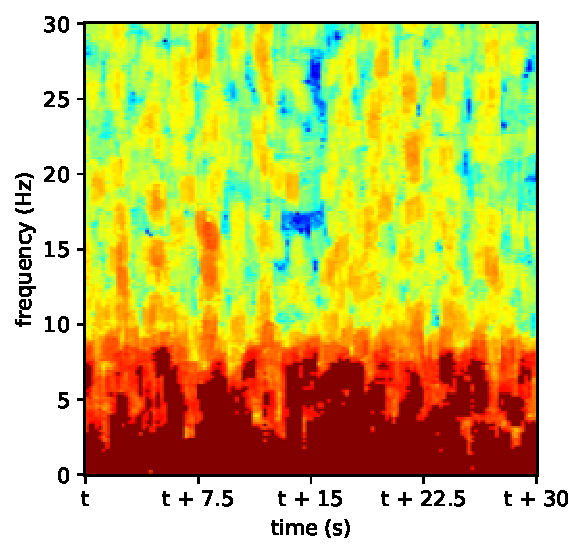
\includegraphics[width=1\linewidth]{./pics/class_clean_0}
  \caption{W}
  \label{fig_1_11}
\end{subfigure}%
\begin{subfigure}{.16\textwidth}
  \centering
  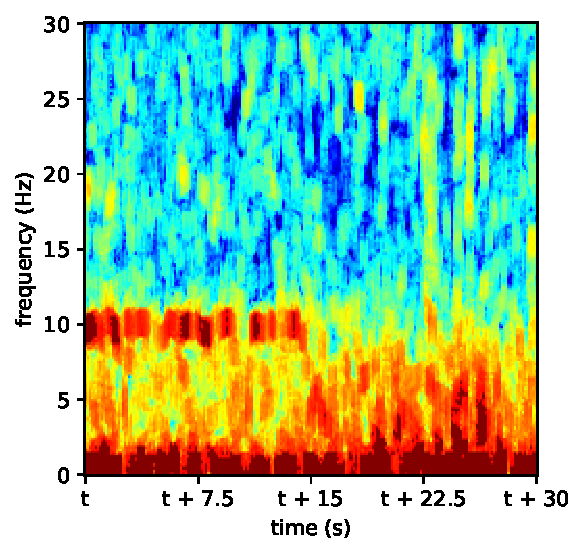
\includegraphics[width=1\linewidth]{./pics/class_clean_1}
  \caption{N1}
  \label{fig_1_12}
\end{subfigure}%
\begin{subfigure}{.16\textwidth}
  \centering
  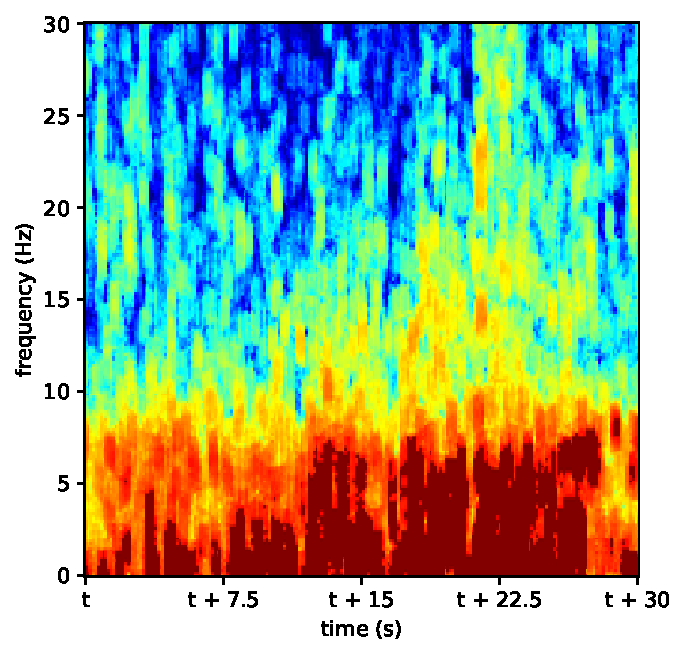
\includegraphics[width=1\linewidth]{./pics/class_clean_2}
  \caption{N2}
  \label{fig_1_13}
\end{subfigure}%
\begin{subfigure}{.16\textwidth}
  \centering
  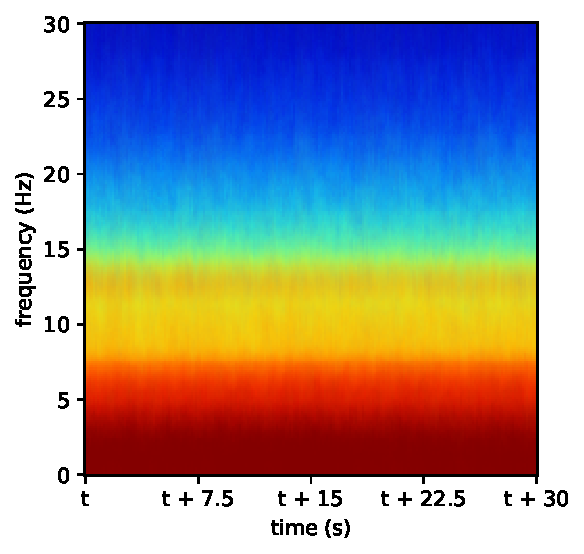
\includegraphics[width=1\linewidth]{./pics/class_clean_3}
  \caption{N3}
  \label{fig_1_14}
\end{subfigure}%
\begin{subfigure}{.16\textwidth}
  \centering
  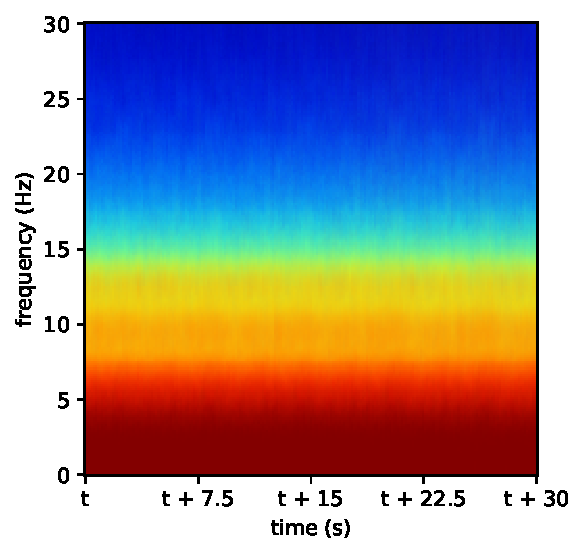
\includegraphics[width=1\linewidth]{./pics/class_clean_4}
  \caption{N4}
  \label{fig_1_15}
\end{subfigure}%
\begin{subfigure}{.16\textwidth}
  \centering
  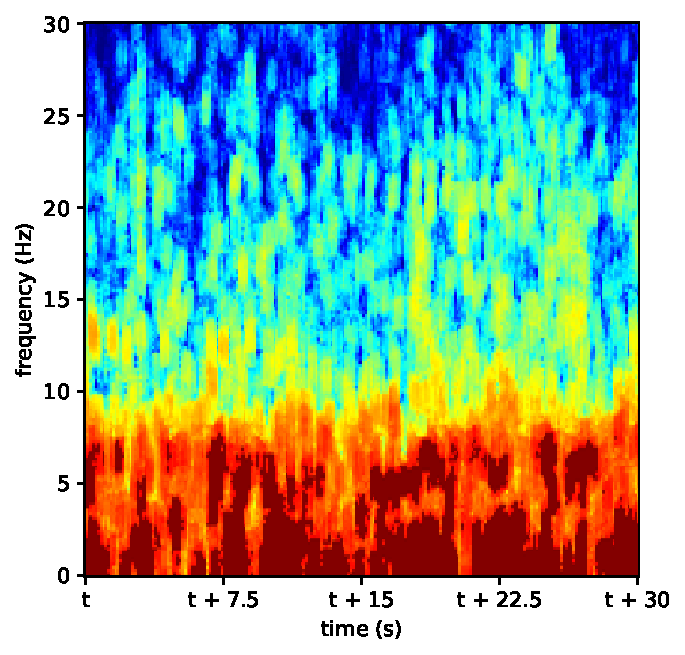
\includegraphics[width=1\linewidth]{./pics/class_clean_5}
  \caption{R}
  \label{fig_1_16}
\end{subfigure}



\begin{subfigure}{.16\textwidth}
  \centering
  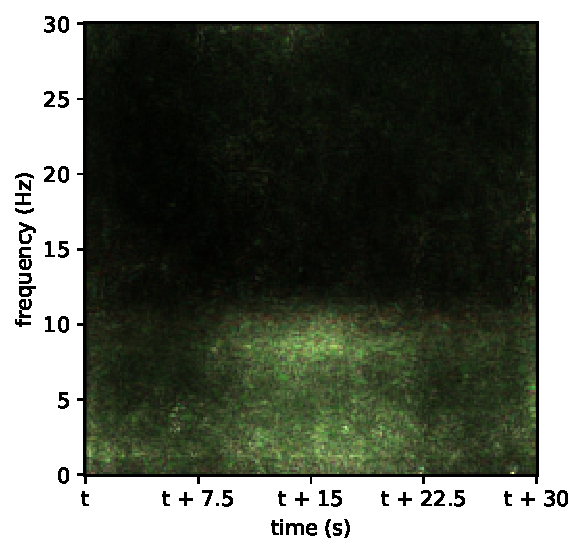
\includegraphics[width=1\linewidth]{./pics/class_master_0}
  \caption{}
  \label{fig_1_21}
\end{subfigure}%
\begin{subfigure}{.16\textwidth}
  \centering
  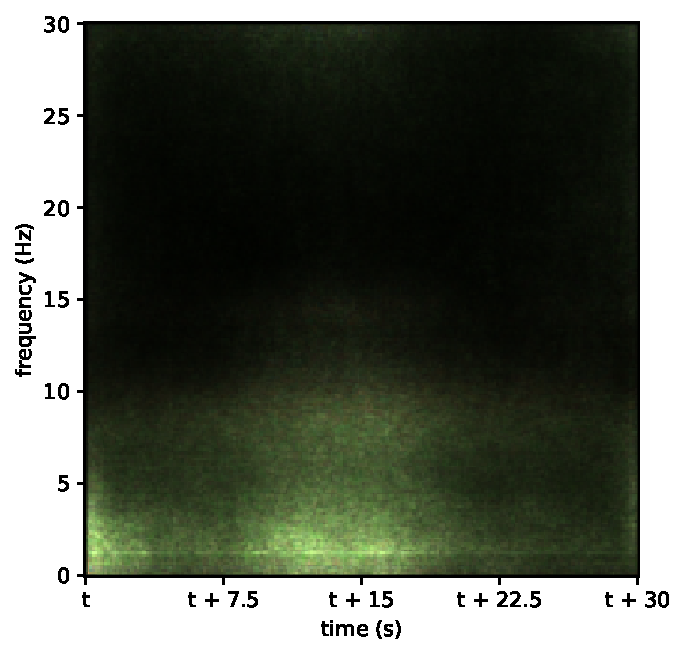
\includegraphics[width=1\linewidth]{./pics/class_master_1}
  \caption{}
  \label{fig_1_22}
\end{subfigure}%
\begin{subfigure}{.16\textwidth}
  \centering
  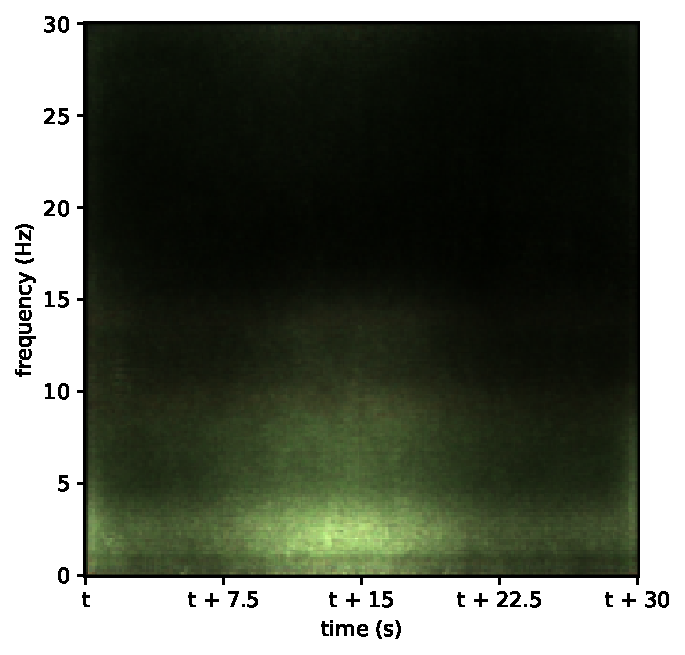
\includegraphics[width=1\linewidth]{./pics/class_master_2}
  \caption{}
  \label{fig_1_23}
\end{subfigure}%
\begin{subfigure}{.16\textwidth}
  \centering
  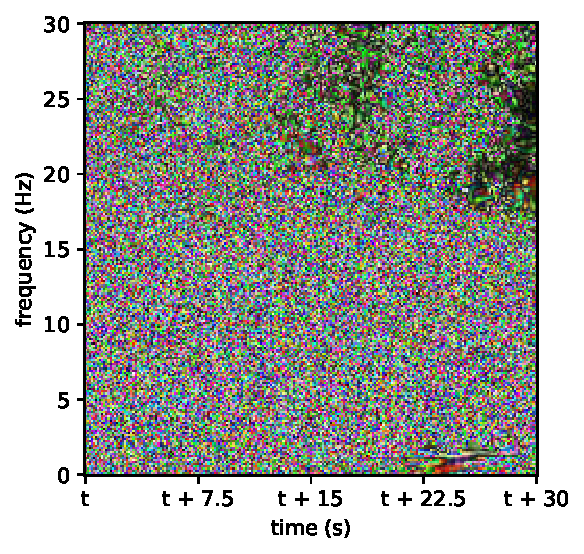
\includegraphics[width=1\linewidth]{./pics/class_master_3}
  \caption{}
  \label{fig_1_24}
\end{subfigure}%
\begin{subfigure}{.16\textwidth}
  \centering
  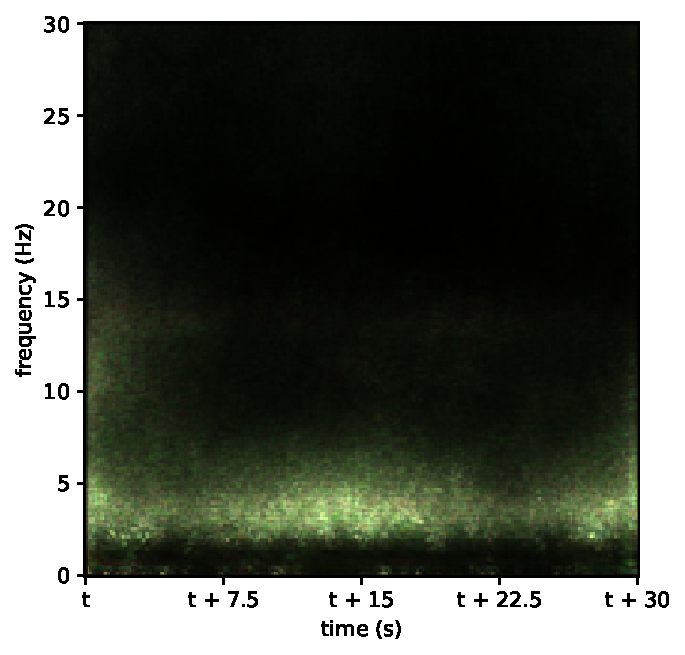
\includegraphics[width=1\linewidth]{./pics/class_master_4}
  \caption{}
  \label{fig_1_25}
\end{subfigure}%
\begin{subfigure}{.16\textwidth}
  \centering
  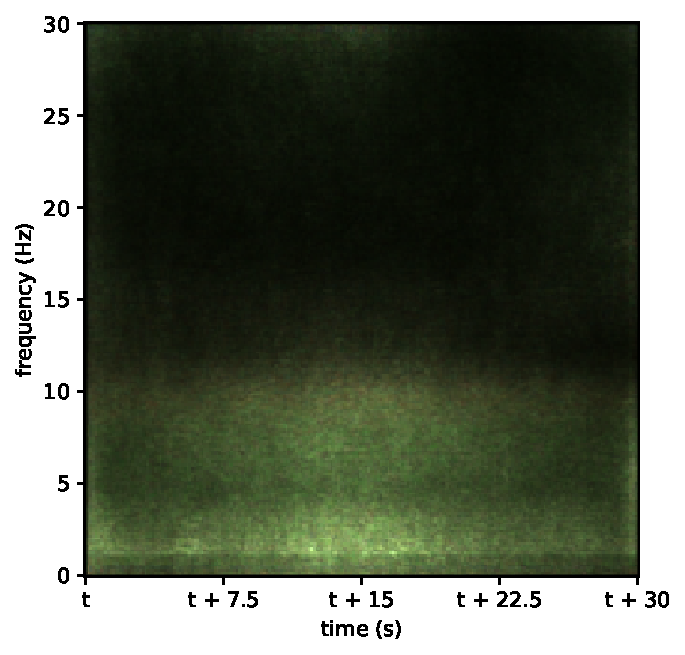
\includegraphics[width=1\linewidth]{./pics/class_master_5}
  \caption{}
  \label{fig_1_26}
\end{subfigure}


\begin{subfigure}{.16\textwidth}
  \centering
  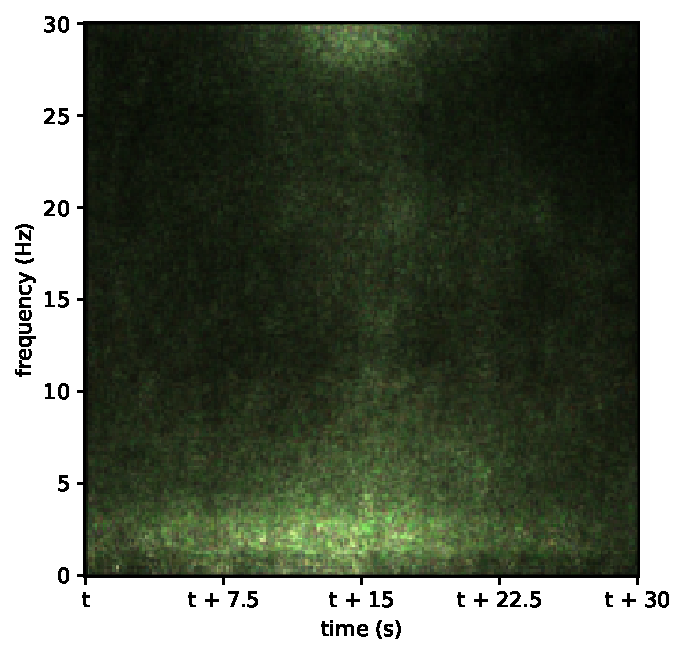
\includegraphics[width=1\linewidth]{./pics/class_rnn_0}
  \caption{}
  \label{fig_1_31}
\end{subfigure}%
\begin{subfigure}{.16\textwidth}
  \centering
  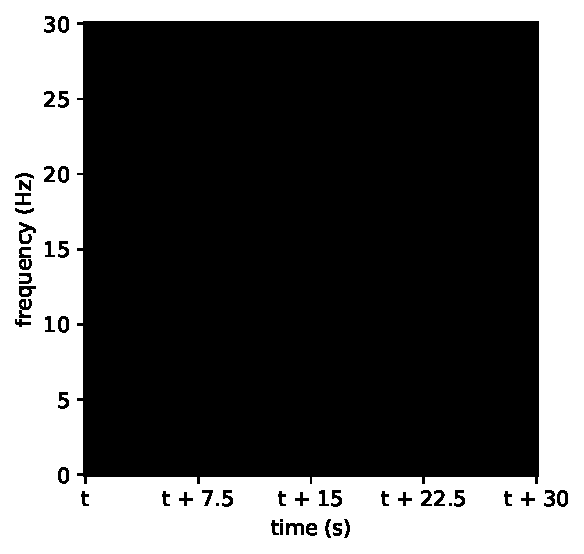
\includegraphics[width=1\linewidth]{./pics/class_rnn_1}
  \caption{}
  \label{fig_1_32}
\end{subfigure}%
\begin{subfigure}{.16\textwidth}
  \centering
  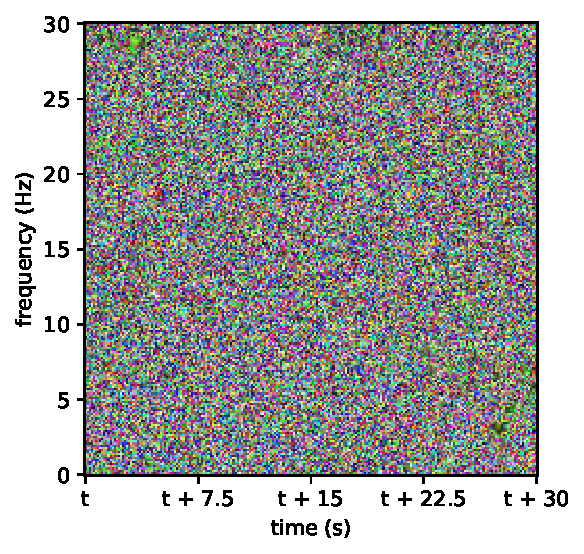
\includegraphics[width=1\linewidth]{./pics/class_rnn_2}
  \caption{}
  \label{fig_1_33}
\end{subfigure}%
\begin{subfigure}{.16\textwidth}
  \centering
  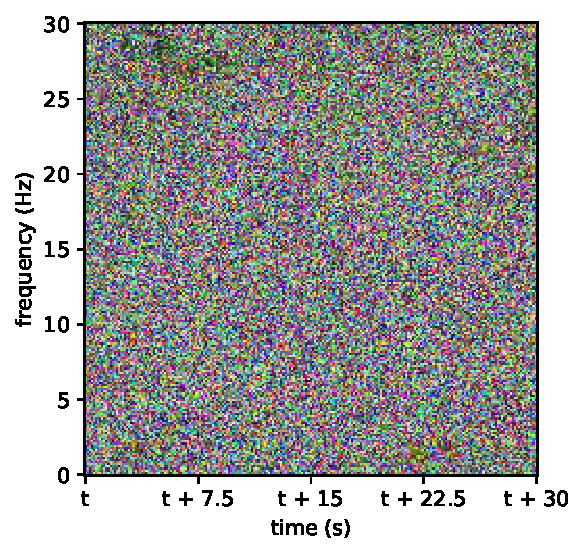
\includegraphics[width=1\linewidth]{./pics/class_rnn_3}
  \caption{}
  \label{fig_1_34}
\end{subfigure}%
\begin{subfigure}{.16\textwidth}
  \centering
  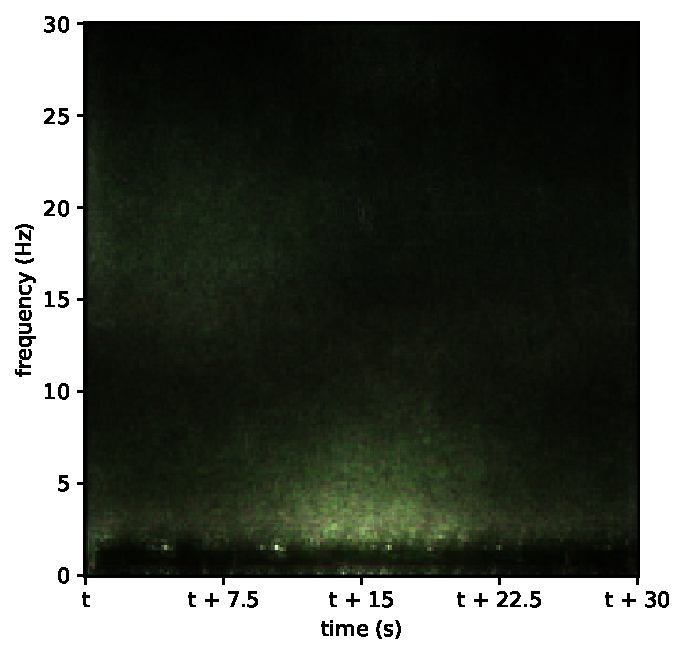
\includegraphics[width=1\linewidth]{./pics/class_rnn_4}
  \caption{}
  \label{fig_1_35}
\end{subfigure}%
\begin{subfigure}{.16\textwidth}
  \centering
  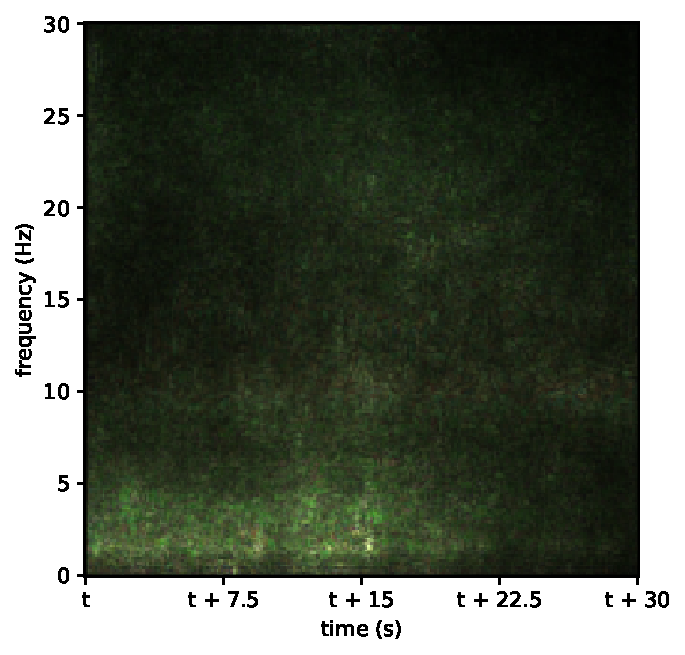
\includegraphics[width=1\linewidth]{./pics/class_rnn_5}
  \caption{}
  \label{fig_1_36}
\end{subfigure}

\caption{This figure contain plots of each sleep stage for the two validation subjects. The visualizations are given columnwise from left to right according to the previous sequence of the sleep stages. Fig. \ref{fig_1_11} to \ref{fig_1_16} illustrate a random epoch of the multi-taper spectrum for each of the sleep stages. There is high similarity between sleep stage N3 and N4.
%(fig. \ref{fig_1_14} and fig. \ref{fig_1_15}). 
The second and the third row, fig \ref{fig_1_21} to \ref{fig_1_36} illustrates the average sensitivity maps of the CNN and of the RNN respectively for the two validation subjects.}
\label{fig_1}
\end{figure*}

The sensitivity maps given in fig. \ref{fig_1_24} - \ref{fig_1_25} and fig. \ref{fig_1_34} - \ref{fig_1_35} for the CNN and the RNN respectively have more less the same pattern. 

The summarized information from the sensitivity maps for sleep stage N3 and N4 provides a valid explanation of the high misclassification error in both networks (see the normalized confusion matrices in table \ref{tab_res_1}).

